\documentclass[14pt,a4paper]{extarticle}

% --- XeLaTeX + Times New Roman (MM-04 §7.1) ---
\usepackage{fontspec}
\usepackage{polyglossia}
\setmainlanguage{english}
\usepackage{graphicx}
\setotherlanguage{russian}
\setmainfont{Times New Roman}
\newfontfamily\cyrillicfont{Times New Roman}

\usepackage{amsmath}
\usepackage{amssymb}

% --- Page geometry per MM-04 §7.2 (30/20/10/25 mm) ---
\usepackage[a4paper,top=20mm,bottom=25mm,left=30mm,right=10mm]{geometry}

% --- Single line spacing and paragraph indentation per MM-04 §7.1 ---
\usepackage{setspace}
\singlespacing
\setlength{\parindent}{1.25cm}
\setlength{\parskip}{0pt}

% --- Normal-control font rule: all visible text is kept at the document
%     base size (14 pt), including title pages, annotations, headings,
%     signatures, tables, and listings. ---
\AtBeginDocument{%
  \let\tiny\normalsize
  \let\scriptsize\normalsize
  \let\footnotesize\normalsize
  \let\small\normalsize
  \let\large\normalsize
  \let\Large\normalsize
  \let\LARGE\normalsize
  \let\huge\normalsize
  \let\Huge\normalsize
}

% --- Microtypography and looser justification to prevent right-margin
%     overflows on long compounds (thermoelastic, three-dimensional,
%     discretisation-invariant, neural-operator, etc.) ---
\usepackage{microtype}
\emergencystretch=3em
\hbadness=10000
\hyphenation{thermo-elastic three-dimen-sional dis-cre-ti-sa-tion neural-operator}

\usepackage{booktabs}
\usepackage{array}
\usepackage{hhline}
\usepackage{float}
\usepackage{flafter}
\usepackage{etoolbox}
\setlength{\intextsep}{\baselineskip}
\setlength{\textfloatsep}{\baselineskip}
\setlength{\floatsep}{\baselineskip}
\usepackage{tikz}
\usetikzlibrary{positioning,arrows.meta,calc,fit,backgrounds}
\usepackage{pgfplots}
\pgfplotsset{compat=1.18}

% --- Captions per MM-04 §7.21 (figures) and §7.24 (tables) ---
\usepackage{xstring}
\usepackage{caption}
\newcommand{\thesisstripcaptionperiod}[1]{%
  \IfEndWith{#1}{.}{\StrGobbleRight{#1}{1}}{#1}%
}
\DeclareCaptionFormat{thesisfigure}{#1#2\thesisstripcaptionperiod{#3}\par}
\DeclareCaptionFormat{thesistable}{\makebox[1.25cm][l]{}#1#2#3\par\vspace{\baselineskip}}
\captionsetup[figure]{name=Figure,labelsep=endash,format=thesisfigure,justification=centering,singlelinecheck=false,font=normalsize,skip=0.5\baselineskip}
\captionsetup[table]{name=Table,labelsep=endash,format=thesistable,justification=raggedright,singlelinecheck=false,font=normalsize,position=above,skip=0pt,belowskip=0pt,margin=0pt}
\renewcommand{\thefigure}{\arabic{figure}}
\renewcommand{\thetable}{\arabic{table}}

% Add left and right borders to tabulars used inside floating tables only.
\makeatletter
\let\thesis@tabular\tabular
\let\endthesis@tabular\endtabular
\newenvironment{thesisborderedtabular}[1]{\thesis@tabular{|#1|}}{\endthesis@tabular}
\AtBeginEnvironment{table}{%
  \let\tabular\thesisborderedtabular
  \let\endtabular\endthesisborderedtabular
}
\makeatother

% --- Section headings ---
\usepackage{titlesec}

\titleformat{\section}[hang]
  {\normalfont\normalsize\bfseries}
  {\thesection}
  {1em}
  {\MakeUppercase}

\titleformat{name=\section,numberless}[block]
  {\normalfont\normalsize\bfseries\filcenter}
  {}
  {0pt}
  {\MakeUppercase}

\titleformat{\subsection}[hang]
  {\normalfont\normalsize\bfseries}
  {\thesubsection}
  {1em}
  {}

\titleformat{\subsubsection}[hang]
  {\normalfont\normalsize\bfseries}
  {\thesubsubsection}
  {1em}
  {}

% После section — 1 пустая строка
\titlespacing*{\section}
  {\parindent}
  {0pt}
  {1\baselineskip}

% Обычные subsection: до заголовка 2 строки, после заголовка 1 строка
\titlespacing*{\subsection}
  {\parindent}
  {2\baselineskip}
  {1\baselineskip}

\titlespacing*{\subsubsection}
  {\parindent}
  {2\baselineskip}
  {1\baselineskip}

% Первый subsection после section:
% убирает дополнительные 2 строки перед subsection,
% потому что section уже дал 1 пустую строку.
\newcommand{\firstsubsection}[1]{%
  {%
    \titlespacing*{\subsection}
      {\parindent}
      {0pt}
      {1\baselineskip}%
    \subsection{#1}%
  }%
}

  
\renewcommand{\thesection}{\arabic{section}}
\renewcommand{\thesubsection}{\thesection.\arabic{subsection}}
\renewcommand{\thesubsubsection}{\thesubsection.\arabic{subsubsection}}
\numberwithin{equation}{section}
\usepackage{indentfirst}

% --- Table of contents formatting. ---
\usepackage{tocloft}
\renewcommand{\cfttoctitlefont}{\normalfont\normalsize}
\renewcommand{\cftaftertoctitle}{\par}
\setlength{\cftbeforetoctitleskip}{0pt}
\setlength{\cftaftertoctitleskip}{\baselineskip}
\renewcommand{\cftsecfont}{\normalfont}
\renewcommand{\cftsecpagefont}{\normalfont}
\renewcommand{\cftsubsecfont}{\normalfont}
\renewcommand{\cftsubsecpagefont}{\normalfont}
\renewcommand{\cftsubsubsecfont}{\normalfont}
\renewcommand{\cftsubsubsecpagefont}{\normalfont}
\renewcommand{\cftsecleader}{\hfill}
\renewcommand{\cftsubsecleader}{\hfill}
\renewcommand{\cftsubsubsecleader}{\hfill}
\setlength{\cftbeforesecskip}{0pt}
\setlength{\cftbeforesubsecskip}{0pt}
\setlength{\cftbeforesubsubsecskip}{0pt}
\cftsetindents{section}{0pt}{2.0cm}
\cftsetindents{subsection}{0pt}{2.0cm}
\cftsetindents{subsubsection}{0pt}{2.0cm}
\makeatletter
\let\thesis@toc@section\l@section
\renewcommand{\l@section}[2]{%
  \thesis@toc@section{\MakeUppercase{#1}}{#2}%
}
\makeatother

\usepackage{tabularx}
\usepackage{booktabs}
\usepackage{array}

% --- IEEE-style numeric citations. ---
\usepackage{cite}
\usepackage[colorlinks=true, allcolors=black]{hyperref}

% --- Source-code listings for the appendices ---
\usepackage{listings}
\usepackage{xcolor}
\definecolor{kw}{HTML}{1F4E79}
\definecolor{str}{HTML}{708050}
\definecolor{cm}{HTML}{777777}
\definecolor{bg}{HTML}{F7F7F2}
\lstdefinestyle{thesiscode}{
  basicstyle=\normalfont\normalsize,
  backgroundcolor=\color{bg},
  keywordstyle=\color{kw}\bfseries,
  stringstyle=\color{str},
  commentstyle=\color{cm}\itshape,
  numbers=left,
  numberstyle=\normalfont\normalsize\color{cm},
  numbersep=6pt,
  frame=single,
  rulecolor=\color{cm!40},
  framesep=4pt,
  tabsize=4,
  showstringspaces=false,
  breaklines=true,
  breakatwhitespace=true,
  columns=fullflexible,
  keepspaces=true,
  upquote=true,
  literate=
    {á}{{\'a}}1 {é}{{\'e}}1 {í}{{\'i}}1 {ó}{{\'o}}1 {ú}{{\'u}}1
    {θ}{{$\theta$}}1 {γ}{{$\gamma$}}1 {ρ}{{$\rho$}}1 {α}{{$\alpha$}}1
    {ν}{{$\nu$}}1 {μ}{{$\mu$}}1 {λ}{{$\lambda$}}1 {σ}{{$\sigma$}}1
}
\lstset{style=thesiscode}

\begin{document}

% Custom title pages. The file tiles.tex must NOT contain
% \documentclass, \begin{document}, or \end{document}.
\thispagestyle{empty}

% ---------------------------------------------------------
% TITLE PAGE
% ---------------------------------------------------------
\begin{center}

{MINISTRY OF SCIENCE AND HIGHER EDUCATION OF THE REPUBLIC OF KAZAKHSTAN}\\
INTERNATIONAL INFORMATION TECHNOLOGY UNIVERSITY\\
FACULTY OF COMPUTER TECHNOLOGIES AND CYBERSECURITY

\vspace{35mm}

Nurshanov D.S.\\
Askarov I.Y.\\
Kassymkhanov T.G.\\
Kaidrakhmetova D.Y.

\vspace{15mm}
\textbf{AI-Guided Prediction of Thermoelastic Wave Propagation in Geological Media}

\vspace{10mm}
{DIPLOMA PROJECT}

\vspace{13mm}
\textbf{Educational Program: 6B06112  Data Science}

\vfill

{Almaty 2026}

\end{center}

\newpage
\thispagestyle{empty}

% ---------------------------------------------------------
% APPROVAL PAGE
% ---------------------------------------------------------
\begin{center}
{MINISTRY OF SCIENCE AND HIGHER EDUCATION OF THE REPUBLIC OF KAZAKHSTAN}\\
INTERNATIONAL INFORMATION TECHNOLOGY UNIVERSITY\\
FACULTY OF COMPUTER TECHNOLOGIES AND CYBERSECURITY\\
DEPARTMENT OF MATHEMATICAL AND COMPUTER MODELING
\end{center}

\vspace{4mm}

\begin{flushright}
\begin{minipage}{6.2cm}
Approved\\
Head of Department,\\
PhD, Associate Professor\\
Abdikalikova Z. T.\\[1mm]
\mbox{\guillemotleft{}\rule{0.8cm}{0.1pt}\guillemotright{}\ \rule{2.2cm}{0.1pt}\ 20\rule{0.4cm}{0.1pt}}
\end{minipage}
\end{flushright}

\vspace{8mm}

\begin{center}
\textbf{DIPLOMA PROJECT}

\vspace{4mm}
\textbf{AI-Guided Prediction of Thermoelastic Wave Propagation in Geological Media}

\vspace{5mm}
\textbf{Educational Program: 6B06112 Data Science}
\end{center}

\vspace{8mm}

\noindent
\begingroup
\setlength{\tabcolsep}{0pt}
\renewcommand{\arraystretch}{1.0}
\begin{tabular*}{\textwidth}{@{\extracolsep{\fill}}l c l@{}}
Done by students: & & \\
Nurshanov D.S. & \rule{3.7cm}{0.1pt} & \mbox{\guillemotleft{}\rule{0.8cm}{0.1pt}\guillemotright{}\ \rule{2.2cm}{0.1pt}\ 20\rule{0.4cm}{0.1pt}} \\
& \small{(signature)} & \\[2mm]
Askarov I.Y. & \rule{3.7cm}{0.1pt} & \mbox{\guillemotleft{}\rule{0.8cm}{0.1pt}\guillemotright{}\ \rule{2.2cm}{0.1pt}\ 20\rule{0.4cm}{0.1pt}} \\
& \small{(signature)} & \\[2mm]
Kassymkhanov T.G. & \rule{3.7cm}{0.1pt} & \mbox{\guillemotleft{}\rule{0.8cm}{0.1pt}\guillemotright{}\ \rule{2.2cm}{0.1pt}\ 20\rule{0.4cm}{0.1pt}} \\
& \small{(signature)} & \\[2mm]
Kaidrakhmetova D.Y. & \rule{3.7cm}{0.1pt} & \mbox{\guillemotleft{}\rule{0.8cm}{0.1pt}\guillemotright{}\ \rule{2.2cm}{0.1pt}\ 20\rule{0.4cm}{0.1pt}} \\
& \small{(signature)} & \\[4mm]
\begin{tabular}[t]{@{}l@{}}
Research advisor:\\
Associate Professor,\\
Candidate of Physical and\\
Mathematical Sciences,\\
PhD in Applied Mathematics\\
Alipova B. N.
\end{tabular}
&
\begin{tabular}[t]{@{}c@{}}
\rule{3.7cm}{0.1pt}\\[-1.5mm]
{\small(signature)}
\end{tabular}
&
\mbox{\guillemotleft{}\rule{0.8cm}{0.1pt}\guillemotright{}\ \rule{2.2cm}{0.1pt}\ 20\rule{0.4cm}{0.1pt}}
\end{tabular*}
\endgroup

\newpage
\thispagestyle{empty}
\enlargethispage{10mm}

% ---------------------------------------------------------
% DIPLOMA PROJECT ASSIGNMENT
% ---------------------------------------------------------
\begin{center}
International Information Technology University\\
Faculty of Computer Technologies and Cybersecurity\\
Department of Mathematical and Computer Modeling
\end{center}

\vspace{9mm}

\noindent Educational Program: 6B06112 -- Data Science

\vspace{4mm}
\noindent Diploma Project Assignment

\vspace{4mm}
\noindent Students\\
\textbf{Nurshanov D.S., Askarov I.Y., Kassymkhanov T.G., Kaidrakhmetova D.Y.}

\vspace{4mm}
\noindent Diploma project topic\\
\textbf{AI-Guided Prediction of Thermoelastic Wave Propagation in Geological Media}

\vspace{4mm}
\noindent Approved by IITU order No. \rule{1.4cm}{0.1pt}\ dated
\hspace{22mm}\mbox{\guillemotleft{}\rule{1cm}{0.1pt}\guillemotright{}\rule{2cm}{0.1pt}20\rule{0.6cm}{0.1pt}}

\vspace{4mm}
\noindent Diploma project submission date
\hspace{38mm}\mbox{\guillemotleft{}\rule{1cm}{0.1pt}\guillemotright{}\rule{2cm}{0.1pt}20\rule{0.6cm}{0.1pt}}

\vspace{4mm}
\noindent Diploma project initial data

\vspace{2mm}
\noindent\underline{Physical and geological parameters of rocks and media, including density,}\\[1mm]
\noindent\underline{elastic properties, thermal expansion, thermal conductivity, and heat capacity.}

\vspace{4mm}
\vspace{4mm}
\noindent Details of computations and explanations (list of issues due to be addressed)

\vspace{2mm}
\noindent\underline{1. Literature review on geological media, thermoelasticity, and elastic wave}\\[1mm]
\noindent\underline{propagation}\\[1mm]
\noindent\underline{2. Analysis of physical and thermal properties of rocks}\\[1mm]
\noindent\underline{3. Mathematical formulation of the thermoelastic wave propagation problem}\\[1mm]
\noindent\underline{4. Analysis of directional behavior in geological media}\\[1mm]
\noindent\underline{5. Preparation of visual materials and interpretation of obtained results}

\vspace{4mm}
\vspace{4mm}
\noindent CD containing the digital version of diploma paper and attachments

\vspace{2mm}
\noindent\rule{\textwidth}{0.1pt}

\clearpage
\thispagestyle{empty}

\vspace{4mm}
\noindent Consultations on diploma project (with related project chapters named)
\vspace{4mm}

\vspace{2mm}
\noindent\begingroup
\setlength{\tabcolsep}{4pt}
\renewcommand{\arraystretch}{1.15}
\begin{tabular}{|>{\centering\arraybackslash}m{3.1cm}|>{\centering\arraybackslash}m{6.0cm}|>{\centering\arraybackslash}m{3.0cm}|>{\centering\arraybackslash}m{3.0cm}|}
\hline
Consultant & Name & \multicolumn{2}{>{\centering\arraybackslash}m{6.15cm}|}{\rule{0pt}{4mm}Signature, date} \\ \cline{3-4}
& & \begin{tabular}{@{}c@{}}Assignment\\given\end{tabular} & \begin{tabular}{@{}c@{}}Assignment\\received\end{tabular} \\ \hline
\begin{tabular}{@{}c@{}}Compliance\\monitor\end{tabular} & \begin{tabular}{@{}c@{}}M.S., Senior Lecturer,\\Srazh A.S.\end{tabular} & & \\[7mm] \hline
\end{tabular}
\endgroup

\vspace{8mm}
\noindent Date \guillemotleft{}\rule{1cm}{0.1pt}\guillemotright{}\rule{2cm}{0.1pt}20\rule{0.6cm}{0.1pt}

\vspace{4mm}
\noindent Research advisor \hfill \rule{7cm}{0.1pt}

\hfill \small{(signature)}

\vspace{2mm}
\noindent Assignment received by \hfill \rule{7cm}{0.1pt}

\hfill \small{(signature)}

\newpage
\thispagestyle{empty}
\enlargethispage{10mm}

% ---------------------------------------------------------
% DIPLOMA PROJECT WRITING SCHEDULE
% ---------------------------------------------------------
\begin{center}
{Diploma project writing schedule}

\vspace{3mm}
\textbf{Nurshanov D.S., Askarov I.Y., Kassymkhanov T.G., Kaidrakhmetova D.Y.}

\vspace{3mm}
\noindent Title: \textbf{AI-Guided Prediction of Thermoelastic Wave Propagation in Geological Media}
\end{center}

\begin{table}[h!]
\centering
\small
\setlength{\tabcolsep}{4pt}
\renewcommand{\arraystretch}{1.15}

\makebox[\textwidth][c]{%
\begin{tabular}{@{}|>{\centering\arraybackslash}m{0.9cm}|m{11.2cm}|>{\centering\arraybackslash}m{3.4cm}|@{}}
\hline
No. & \centering\arraybackslash Assignment & Period \\ \hline
1 & Creation of the graduation paper writing schedule & September 15 \\ \hline
2 & Collection and analysis of theoretical and geological information & November \\ \hline
3 & Study of thermoelasticity, heat conduction, and elastic wave propagation theory (Introduction, Chapters 1-4) & December \\ \hline
4 & Mathematical formulation of the thermoelastic wave propagation problem & January \\ \hline
5 & Analysis of Existing Models and Approaches (Chapter 5) & January -- February \\ \hline
6 & Development and Implementation of Predictive Models & March -- April \\ \hline
7 & Preparation of visual materials, analysis, and interpretation (Chapters 6, 7) & May \\ \hline
8 & First pre-defense & April 11 \\ \hline
9 & Second pre-defense & May 18 \\ \hline
10 & Submission of the diploma paper for plagiarism check & May 11--15 \\ \hline
11 & Submission of the diploma paper to the compliance monitor & May 16--25 \\ \hline
12 & Submission to the reviewer for approval & May 28 \\ \hline
13 & Diploma project defense & June 1--5 \\ \hline
\end{tabular}%
}
\end{table}
\vspace{1mm}

\noindent\begingroup
\setlength{\tabcolsep}{0pt}
\renewcommand{\arraystretch}{1.00}
\begin{tabular}{@{}p{10.4cm}>{\centering\arraybackslash}p{4.8cm}@{}}
Student: Nurshanov D.S. & \rule{4cm}{0.1pt} \\
& \small{(signature)} \\
Student: Askarov I.Y. & \rule{4cm}{0.1pt} \\
& \small{(signature)} \\
Student: Kassymkhanov T.G. & \rule{4cm}{0.1pt} \\
& \small{(signature)} \\
Student: Kaidrakhmetova D.Y. & \rule{4cm}{0.1pt} \\
& \small{(signature)} \\
Research advisor: Alipova B. N. & \rule{4cm}{0.1pt} \\
& \small{(signature)}
\end{tabular}
\endgroup

\vspace{1mm}
\noindent Date \guillemotleft{}\rule{1cm}{0.1pt}\guillemotright{}\ \rule{1.5cm}{0.1pt}\ 20\rule{0.5cm}{0.1pt}


% Abstracts / annotations with count fields.
% annotation_counts.tex
% Supplies annotation statistics for the three annotation pages.

\newcounter{annotationmetric}
\let\annotationnormalrule\rule
\newcommand{\annotationmetricrule}[2]{%
  \stepcounter{annotationmetric}%
  \ifcase\value{annotationmetric}%
    \annotationnormalrule{#1}{#2}%
  \or 174% pages, Kazakh
  \or 9% tables, Kazakh
  \or 27% illustrations, Kazakh
  \or 27% references, Kazakh
  \or 174% pages, Russian
  \or 9% tables, Russian
  \or 27% illustrations, Russian
  \or 27% references, Russian
  \or 174% pages, English
  \or 9% tables, English
  \or 27% illustrations, English
  \or 27% references, English
  \else \annotationnormalrule{#1}{#2}%
  \fi
}

\makeatletter
\let\annotationnormaltextbf\textbf
\def\annotationkazkeywords{Кілт сөздер:}
\def\annotationruskeywords{Перечень ключевых слов:}
\def\annotationengkeywords{Keywords:}
\def\annotationlowerkeywords#1.{\MakeLowercase{#1}.}
\renewcommand{\textbf}[1]{%
  \def\annotationcurrentlabel{#1}%
  \annotationnormaltextbf{#1}%
  \ifx\annotationcurrentlabel\annotationkazkeywords
    \expandafter\annotationlowerkeywords
  \else\ifx\annotationcurrentlabel\annotationruskeywords
    \expandafter\annotationlowerkeywords
  \else\ifx\annotationcurrentlabel\annotationengkeywords
    \expandafter\annotationlowerkeywords
  \fi\fi\fi
}
\makeatother

\renewcommand{\rule}[2]{\annotationmetricrule{#1}{#2}}
\begingroup
\sloppy
\tolerance=3000
\emergencystretch=8em
\hyphenpenalty=50
\exhyphenpenalty=50
% annotations.tex
% This file should be included after the title pages:
% \thispagestyle{empty}

% ---------------------------------------------------------
% TITLE PAGE
% ---------------------------------------------------------
\begin{center}

{MINISTRY OF SCIENCE AND HIGHER EDUCATION OF THE REPUBLIC OF KAZAKHSTAN}\\
INTERNATIONAL INFORMATION TECHNOLOGY UNIVERSITY\\
FACULTY OF COMPUTER TECHNOLOGIES AND CYBERSECURITY

\vspace{35mm}

Nurshanov D.S.\\
Askarov I.Y.\\
Kassymkhanov T.G.\\
Kaidrakhmetova D.Y.

\vspace{15mm}
\textbf{AI-Guided Prediction of Thermoelastic Wave Propagation in Geological Media}

\vspace{10mm}
{DIPLOMA PROJECT}

\vspace{13mm}
\textbf{Educational Program: 6B06112  Data Science}

\vfill

{Almaty 2026}

\end{center}

\newpage
\thispagestyle{empty}

% ---------------------------------------------------------
% APPROVAL PAGE
% ---------------------------------------------------------
\begin{center}
{MINISTRY OF SCIENCE AND HIGHER EDUCATION OF THE REPUBLIC OF KAZAKHSTAN}\\
INTERNATIONAL INFORMATION TECHNOLOGY UNIVERSITY\\
FACULTY OF COMPUTER TECHNOLOGIES AND CYBERSECURITY\\
DEPARTMENT OF MATHEMATICAL AND COMPUTER MODELING
\end{center}

\vspace{4mm}

\begin{flushright}
\begin{minipage}{6.2cm}
Approved\\
Head of Department,\\
PhD, Associate Professor\\
Abdikalikova Z. T.\\[1mm]
\mbox{\guillemotleft{}\rule{0.8cm}{0.1pt}\guillemotright{}\ \rule{2.2cm}{0.1pt}\ 20\rule{0.4cm}{0.1pt}}
\end{minipage}
\end{flushright}

\vspace{8mm}

\begin{center}
\textbf{DIPLOMA PROJECT}

\vspace{4mm}
\textbf{AI-Guided Prediction of Thermoelastic Wave Propagation in Geological Media}

\vspace{5mm}
\textbf{Educational Program: 6B06112 Data Science}
\end{center}

\vspace{8mm}

\noindent
\begingroup
\setlength{\tabcolsep}{0pt}
\renewcommand{\arraystretch}{1.0}
\begin{tabular*}{\textwidth}{@{\extracolsep{\fill}}l c l@{}}
Done by students: & & \\
Nurshanov D.S. & \rule{3.7cm}{0.1pt} & \mbox{\guillemotleft{}\rule{0.8cm}{0.1pt}\guillemotright{}\ \rule{2.2cm}{0.1pt}\ 20\rule{0.4cm}{0.1pt}} \\
& \small{(signature)} & \\[2mm]
Askarov I.Y. & \rule{3.7cm}{0.1pt} & \mbox{\guillemotleft{}\rule{0.8cm}{0.1pt}\guillemotright{}\ \rule{2.2cm}{0.1pt}\ 20\rule{0.4cm}{0.1pt}} \\
& \small{(signature)} & \\[2mm]
Kassymkhanov T.G. & \rule{3.7cm}{0.1pt} & \mbox{\guillemotleft{}\rule{0.8cm}{0.1pt}\guillemotright{}\ \rule{2.2cm}{0.1pt}\ 20\rule{0.4cm}{0.1pt}} \\
& \small{(signature)} & \\[2mm]
Kaidrakhmetova D.Y. & \rule{3.7cm}{0.1pt} & \mbox{\guillemotleft{}\rule{0.8cm}{0.1pt}\guillemotright{}\ \rule{2.2cm}{0.1pt}\ 20\rule{0.4cm}{0.1pt}} \\
& \small{(signature)} & \\[4mm]
\begin{tabular}[t]{@{}l@{}}
Research advisor:\\
Associate Professor,\\
Candidate of Physical and\\
Mathematical Sciences,\\
PhD in Applied Mathematics\\
Alipova B. N.
\end{tabular}
&
\begin{tabular}[t]{@{}c@{}}
\rule{3.7cm}{0.1pt}\\[-1.5mm]
{\small(signature)}
\end{tabular}
&
\mbox{\guillemotleft{}\rule{0.8cm}{0.1pt}\guillemotright{}\ \rule{2.2cm}{0.1pt}\ 20\rule{0.4cm}{0.1pt}}
\end{tabular*}
\endgroup

\newpage
\thispagestyle{empty}
\enlargethispage{10mm}

% ---------------------------------------------------------
% DIPLOMA PROJECT ASSIGNMENT
% ---------------------------------------------------------
\begin{center}
International Information Technology University\\
Faculty of Computer Technologies and Cybersecurity\\
Department of Mathematical and Computer Modeling
\end{center}

\vspace{9mm}

\noindent Educational Program: 6B06112 -- Data Science

\vspace{4mm}
\noindent Diploma Project Assignment

\vspace{4mm}
\noindent Students\\
\textbf{Nurshanov D.S., Askarov I.Y., Kassymkhanov T.G., Kaidrakhmetova D.Y.}

\vspace{4mm}
\noindent Diploma project topic\\
\textbf{AI-Guided Prediction of Thermoelastic Wave Propagation in Geological Media}

\vspace{4mm}
\noindent Approved by IITU order No. \rule{1.4cm}{0.1pt}\ dated
\hspace{22mm}\mbox{\guillemotleft{}\rule{1cm}{0.1pt}\guillemotright{}\rule{2cm}{0.1pt}20\rule{0.6cm}{0.1pt}}

\vspace{4mm}
\noindent Diploma project submission date
\hspace{38mm}\mbox{\guillemotleft{}\rule{1cm}{0.1pt}\guillemotright{}\rule{2cm}{0.1pt}20\rule{0.6cm}{0.1pt}}

\vspace{4mm}
\noindent Diploma project initial data

\vspace{2mm}
\noindent\underline{Physical and geological parameters of rocks and media, including density,}\\[1mm]
\noindent\underline{elastic properties, thermal expansion, thermal conductivity, and heat capacity.}

\vspace{4mm}
\vspace{4mm}
\noindent Details of computations and explanations (list of issues due to be addressed)

\vspace{2mm}
\noindent\underline{1. Literature review on geological media, thermoelasticity, and elastic wave}\\[1mm]
\noindent\underline{propagation}\\[1mm]
\noindent\underline{2. Analysis of physical and thermal properties of rocks}\\[1mm]
\noindent\underline{3. Mathematical formulation of the thermoelastic wave propagation problem}\\[1mm]
\noindent\underline{4. Analysis of directional behavior in geological media}\\[1mm]
\noindent\underline{5. Preparation of visual materials and interpretation of obtained results}

\vspace{4mm}
\vspace{4mm}
\noindent CD containing the digital version of diploma paper and attachments

\vspace{2mm}
\noindent\rule{\textwidth}{0.1pt}

\clearpage
\thispagestyle{empty}

\vspace{4mm}
\noindent Consultations on diploma project (with related project chapters named)
\vspace{4mm}

\vspace{2mm}
\noindent\begingroup
\setlength{\tabcolsep}{4pt}
\renewcommand{\arraystretch}{1.15}
\begin{tabular}{|>{\centering\arraybackslash}m{3.1cm}|>{\centering\arraybackslash}m{6.0cm}|>{\centering\arraybackslash}m{3.0cm}|>{\centering\arraybackslash}m{3.0cm}|}
\hline
Consultant & Name & \multicolumn{2}{>{\centering\arraybackslash}m{6.15cm}|}{\rule{0pt}{4mm}Signature, date} \\ \cline{3-4}
& & \begin{tabular}{@{}c@{}}Assignment\\given\end{tabular} & \begin{tabular}{@{}c@{}}Assignment\\received\end{tabular} \\ \hline
\begin{tabular}{@{}c@{}}Compliance\\monitor\end{tabular} & \begin{tabular}{@{}c@{}}M.S., Senior Lecturer,\\Srazh A.S.\end{tabular} & & \\[7mm] \hline
\end{tabular}
\endgroup

\vspace{8mm}
\noindent Date \guillemotleft{}\rule{1cm}{0.1pt}\guillemotright{}\rule{2cm}{0.1pt}20\rule{0.6cm}{0.1pt}

\vspace{4mm}
\noindent Research advisor \hfill \rule{7cm}{0.1pt}

\hfill \small{(signature)}

\vspace{2mm}
\noindent Assignment received by \hfill \rule{7cm}{0.1pt}

\hfill \small{(signature)}

\newpage
\thispagestyle{empty}
\enlargethispage{10mm}

% ---------------------------------------------------------
% DIPLOMA PROJECT WRITING SCHEDULE
% ---------------------------------------------------------
\begin{center}
{Diploma project writing schedule}

\vspace{3mm}
\textbf{Nurshanov D.S., Askarov I.Y., Kassymkhanov T.G., Kaidrakhmetova D.Y.}

\vspace{3mm}
\noindent Title: \textbf{AI-Guided Prediction of Thermoelastic Wave Propagation in Geological Media}
\end{center}

\begin{table}[h!]
\centering
\small
\setlength{\tabcolsep}{4pt}
\renewcommand{\arraystretch}{1.15}

\makebox[\textwidth][c]{%
\begin{tabular}{@{}|>{\centering\arraybackslash}m{0.9cm}|m{11.2cm}|>{\centering\arraybackslash}m{3.4cm}|@{}}
\hline
No. & \centering\arraybackslash Assignment & Period \\ \hline
1 & Creation of the graduation paper writing schedule & September 15 \\ \hline
2 & Collection and analysis of theoretical and geological information & November \\ \hline
3 & Study of thermoelasticity, heat conduction, and elastic wave propagation theory (Introduction, Chapters 1-4) & December \\ \hline
4 & Mathematical formulation of the thermoelastic wave propagation problem & January \\ \hline
5 & Analysis of Existing Models and Approaches (Chapter 5) & January -- February \\ \hline
6 & Development and Implementation of Predictive Models & March -- April \\ \hline
7 & Preparation of visual materials, analysis, and interpretation (Chapters 6, 7) & May \\ \hline
8 & First pre-defense & April 11 \\ \hline
9 & Second pre-defense & May 18 \\ \hline
10 & Submission of the diploma paper for plagiarism check & May 11--15 \\ \hline
11 & Submission of the diploma paper to the compliance monitor & May 16--25 \\ \hline
12 & Submission to the reviewer for approval & May 28 \\ \hline
13 & Diploma project defense & June 1--5 \\ \hline
\end{tabular}%
}
\end{table}
\vspace{1mm}

\noindent\begingroup
\setlength{\tabcolsep}{0pt}
\renewcommand{\arraystretch}{1.00}
\begin{tabular}{@{}p{10.4cm}>{\centering\arraybackslash}p{4.8cm}@{}}
Student: Nurshanov D.S. & \rule{4cm}{0.1pt} \\
& \small{(signature)} \\
Student: Askarov I.Y. & \rule{4cm}{0.1pt} \\
& \small{(signature)} \\
Student: Kassymkhanov T.G. & \rule{4cm}{0.1pt} \\
& \small{(signature)} \\
Student: Kaidrakhmetova D.Y. & \rule{4cm}{0.1pt} \\
& \small{(signature)} \\
Research advisor: Alipova B. N. & \rule{4cm}{0.1pt} \\
& \small{(signature)}
\end{tabular}
\endgroup

\vspace{1mm}
\noindent Date \guillemotleft{}\rule{1cm}{0.1pt}\guillemotright{}\ \rule{1.5cm}{0.1pt}\ 20\rule{0.5cm}{0.1pt}

% % annotations.tex
% This file should be included after the title pages:
% \input{tiles.tex}
% \input{annotations.tex}

\clearpage
\thispagestyle{empty}

\begin{center}
\textbf{\Large АҢДАТПА}
\end{center}

Дипломдық жобаның мақсаты геологиялық ортада термосерпімді толқындардың таралу бағытын болжауға арналған теориялық және есептеу негізін әзірлеу болып табылады. Жұмыста тау жыныстары табиғи қатты денелер ретінде қарастырылып, олардың физикалық мінез-құлқы минералдық құрамға, тығыздыққа, кеуектілікке, серпімділік қасиеттеріне, жылу өткізгіштікке, жылу сыйымдылығына, термиялық ұлғаю коэффициентіне, температуралық жағдайға және кернеулік күйге тәуелді екені сипатталады.

Жобаның теориялық бөлігі термосерпімділік, жылу өткізгіштік, термиялық кернеу, серпімді деформация және геологиялық ортадағы толқындардың таралуы арасындағы байланысты түсіндіруге бағытталған. Ерекше назар қабаттылық, жарықшақтар, кеуектер, анизотропия және жыныстың ішкі құрылымы толқындардың бағытқа тәуелді таралуына қалай әсер ететініне аударылады. Температураның өзгеруі еркін ұлғаю немесе сығылу ғана емес, геологиялық шектеулер жағдайында қосымша термиялық кернеулер тудыруы мүмкін екені көрсетіледі.

Практикалық бөлік геологиялық материалдардың физикалық параметрлеріне сүйене отырып, термосерпімді толқындардың таралу бағытын салыстырмалы түрде талдауға арналған прототиптік тәсілді қарастырады. Бұл жұмыс нақты далалық геофизикалық модельдеуді толық алмастыруды мақсат етпейді; оның негізгі міндеті — геологиялық ортадағы жылулық және механикалық процестердің байланысын теориялық тұрғыдан негіздеп, бағыттық толқындық мінез-құлықты түсіндіруге арналған құрылымдалған негіз ұсыну.

Дипломдық жобада \rule{1cm}{0.1pt} бет, \rule{1cm}{0.1pt} кесте, \rule{1cm}{0.1pt} сурет және \rule{1cm}{0.1pt} пайдаланылған әдебиеттер бар.

\vspace{5mm}
\noindent\textbf{Кілт сөздер тізімі:} ТЕРМОСЕРПІМДІЛІК, ГЕОЛОГИЯЛЫҚ ОРТА, СЕРПІМДІ ТОЛҚЫНДАР, ЖЫЛУ ӨТКІЗГІШТІК, ТЕРМИЯЛЫҚ КЕРНЕУ, ТАУ ЖЫНЫСТАРЫ, БАҒЫТТЫҚ ТАРАЛУ, АНИЗОТРОПИЯ, ГЕОФИЗИКА, ЖАСАНДЫ ИНТЕЛЛЕКТ.

\clearpage
\thispagestyle{empty}

\begin{center}
\textbf{\Large АННОТАЦИЯ}
\end{center}

Целью дипломного проекта является разработка и теоретическое обоснование подхода к направленному прогнозированию распространения термоупругих волн в геологических средах. В работе геологические среды рассматриваются как природные твердые материалы, физическое поведение которых зависит от минерального состава, плотности, пористости, упругих свойств, теплопроводности, теплоемкости, коэффициента теплового расширения, температурного режима и напряженного состояния.

Теоретическая часть проекта направлена на объяснение связи между термоупругостью, теплопроводностью, тепловыми напряжениями, упругой деформацией и распространением волн в горных породах. Особое внимание уделяется тому, как слоистость, трещиноватость, поровая структура, анизотропия и внутренняя структура пород влияют на направленное поведение волн. Показано, что изменение температуры может приводить не только к свободному расширению или сжатию, но и к возникновению дополнительных тепловых напряжений при наличии геологических ограничений.

Практическая часть работы рассматривает прототипный подход к сравнительному анализу направления распространения термоупругих волн на основе физических параметров геологических материалов. Работа не претендует на полную замену реального полевого геофизического моделирования; ее основная задача состоит в теоретическом обосновании связи тепловых и механических процессов в геологической среде и в формировании структурированной основы для интерпретации направленного волнового поведения.

Дипломный проект содержит \rule{1cm}{0.1pt} страниц, \rule{1cm}{0.1pt} таблиц, \rule{1cm}{0.1pt} иллюстраций и \rule{1cm}{0.1pt} использованных источников.

\vspace{5mm}
\noindent\textbf{Перечень ключевых слов:} ТЕРМОУПРУГОСТЬ, ГЕОЛОГИЧЕСКАЯ СРЕДА, УПРУГИЕ ВОЛНЫ, ТЕПЛОПРОВОДНОСТЬ, ТЕПЛОВОЕ НАПРЯЖЕНИЕ, ГОРНЫЕ ПОРОДЫ, НАПРАВЛЕННОЕ РАСПРОСТРАНЕНИЕ, АНИЗОТРОПИЯ, ГЕОФИЗИКА, ИСКУССТВЕННЫЙ ИНТЕЛЛЕКТ.

\clearpage
\thispagestyle{empty}

\begin{center}
\textbf{\Large ABSTRACT}
\end{center}

The aim of the diploma project is to develop and theoretically justify an approach to directional prediction of thermoelastic wave propagation in geological media. Geological media are considered as natural solid materials whose physical behavior depends on mineral composition, density, porosity, elastic properties, thermal conductivity, heat capacity, coefficient of thermal expansion, temperature conditions, and stress state.

The theoretical part of the project explains the relationship between thermoelasticity, heat conduction, thermal stress, elastic deformation, and wave propagation in rocks. Particular attention is given to the influence of layering, fractures, pore structure, anisotropy, and internal rock fabric on directional wave behavior. The work emphasizes that temperature changes may cause not only free expansion or contraction, but also additional thermal stresses when geological constraints are present.

The practical part considers a prototype-oriented approach for comparative analysis of the direction of thermoelastic wave propagation based on physical parameters of geological materials. The work does not claim to replace full-scale field geophysical modelling. Its main purpose is to provide a theoretical explanation of the interaction between thermal and mechanical processes in geological media and to form a structured basis for interpreting directional wave behavior.

The graduation project contains \rule{1cm}{0.1pt} pages, \rule{1cm}{0.1pt} tables, \rule{1cm}{0.1pt} illustrations, and \rule{1cm}{0.1pt} references.

\vspace{5mm}
\noindent\textbf{Keywords:} THERMOELASTICITY, GEOLOGICAL MEDIA, ELASTIC WAVES, HEAT CONDUCTION, THERMAL STRESS, ROCKS, DIRECTIONAL PROPAGATION, ANISOTROPY, GEOPHYSICS, ARTIFICIAL INTELLIGENCE.


\clearpage
\thispagestyle{empty}

\begin{center}
\textbf{\Large АҢДАТПА}
\end{center}

Дипломдық жобаның мақсаты геологиялық ортада термосерпімді толқындардың таралу бағытын болжауға арналған теориялық және есептеу негізін әзірлеу болып табылады. Жұмыста тау жыныстары табиғи қатты денелер ретінде қарастырылып, олардың физикалық мінез-құлқы минералдық құрамға, тығыздыққа, кеуектілікке, серпімділік қасиеттеріне, жылу өткізгіштікке, жылу сыйымдылығына, термиялық ұлғаю коэффициентіне, температуралық жағдайға және кернеулік күйге тәуелді екені сипатталады.

Жобаның теориялық бөлігі термосерпімділік, жылу өткізгіштік, термиялық кернеу, серпімді деформация және геологиялық ортадағы толқындардың таралуы арасындағы байланысты түсіндіруге бағытталған. Ерекше назар қабаттылық, жарықшақтар, кеуектер, анизотропия және жыныстың ішкі құрылымы толқындардың бағытқа тәуелді таралуына қалай әсер ететініне аударылады. Температураның өзгеруі еркін ұлғаю немесе сығылу ғана емес, геологиялық шектеулер жағдайында қосымша термиялық кернеулер тудыруы мүмкін екені көрсетіледі.

Практикалық бөлік геологиялық материалдардың физикалық параметрлеріне сүйене отырып, термосерпімді толқындардың таралу бағытын салыстырмалы түрде талдауға арналған прототиптік тәсілді қарастырады. Бұл жұмыс нақты далалық геофизикалық модельдеуді толық алмастыруды мақсат етпейді; оның негізгі міндеті — геологиялық ортадағы жылулық және механикалық процестердің байланысын теориялық тұрғыдан негіздеп, бағыттық толқындық мінез-құлықты түсіндіруге арналған құрылымдалған негіз ұсыну.

Дипломдық жобада \rule{1cm}{0.1pt} бет, \rule{1cm}{0.1pt} кесте, \rule{1cm}{0.1pt} сурет және \rule{1cm}{0.1pt} пайдаланылған әдебиеттер бар.

\vspace{5mm}
\noindent\textbf{Кілт сөздер тізімі:} ТЕРМОСЕРПІМДІЛІК, ГЕОЛОГИЯЛЫҚ ОРТА, СЕРПІМДІ ТОЛҚЫНДАР, ЖЫЛУ ӨТКІЗГІШТІК, ТЕРМИЯЛЫҚ КЕРНЕУ, ТАУ ЖЫНЫСТАРЫ, БАҒЫТТЫҚ ТАРАЛУ, АНИЗОТРОПИЯ, ГЕОФИЗИКА, ЖАСАНДЫ ИНТЕЛЛЕКТ.

\clearpage
\thispagestyle{empty}

\begin{center}
\textbf{\Large АННОТАЦИЯ}
\end{center}

Целью дипломного проекта является разработка и теоретическое обоснование подхода к направленному прогнозированию распространения термоупругих волн в геологических средах. В работе геологические среды рассматриваются как природные твердые материалы, физическое поведение которых зависит от минерального состава, плотности, пористости, упругих свойств, теплопроводности, теплоемкости, коэффициента теплового расширения, температурного режима и напряженного состояния.

Теоретическая часть проекта направлена на объяснение связи между термоупругостью, теплопроводностью, тепловыми напряжениями, упругой деформацией и распространением волн в горных породах. Особое внимание уделяется тому, как слоистость, трещиноватость, поровая структура, анизотропия и внутренняя структура пород влияют на направленное поведение волн. Показано, что изменение температуры может приводить не только к свободному расширению или сжатию, но и к возникновению дополнительных тепловых напряжений при наличии геологических ограничений.

Практическая часть работы рассматривает прототипный подход к сравнительному анализу направления распространения термоупругих волн на основе физических параметров геологических материалов. Работа не претендует на полную замену реального полевого геофизического моделирования; ее основная задача состоит в теоретическом обосновании связи тепловых и механических процессов в геологической среде и в формировании структурированной основы для интерпретации направленного волнового поведения.

Дипломный проект содержит \rule{1cm}{0.1pt} страниц, \rule{1cm}{0.1pt} таблиц, \rule{1cm}{0.1pt} иллюстраций и \rule{1cm}{0.1pt} использованных источников.

\vspace{5mm}
\noindent\textbf{Перечень ключевых слов:} ТЕРМОУПРУГОСТЬ, ГЕОЛОГИЧЕСКАЯ СРЕДА, УПРУГИЕ ВОЛНЫ, ТЕПЛОПРОВОДНОСТЬ, ТЕПЛОВОЕ НАПРЯЖЕНИЕ, ГОРНЫЕ ПОРОДЫ, НАПРАВЛЕННОЕ РАСПРОСТРАНЕНИЕ, АНИЗОТРОПИЯ, ГЕОФИЗИКА, ИСКУССТВЕННЫЙ ИНТЕЛЛЕКТ.

\clearpage
\thispagestyle{empty}

\begin{center}
\textbf{\Large ABSTRACT}
\end{center}

The aim of the diploma project is to develop and theoretically justify an approach to directional prediction of thermoelastic wave propagation in geological media. Geological media are considered as natural solid materials whose physical behavior depends on mineral composition, density, porosity, elastic properties, thermal conductivity, heat capacity, coefficient of thermal expansion, temperature conditions, and stress state.

The theoretical part of the project explains the relationship between thermoelasticity, heat conduction, thermal stress, elastic deformation, and wave propagation in rocks. Particular attention is given to the influence of layering, fractures, pore structure, anisotropy, and internal rock fabric on directional wave behavior. The work emphasizes that temperature changes may cause not only free expansion or contraction, but also additional thermal stresses when geological constraints are present.

The practical part considers a prototype-oriented approach for comparative analysis of the direction of thermoelastic wave propagation based on physical parameters of geological materials. The work does not claim to replace full-scale field geophysical modelling. Its main purpose is to provide a theoretical explanation of the interaction between thermal and mechanical processes in geological media and to form a structured basis for interpreting directional wave behavior.

The graduation project contains \rule{1cm}{0.1pt} pages, \rule{1cm}{0.1pt} tables, \rule{1cm}{0.1pt} illustrations, and \rule{1cm}{0.1pt} references.

\vspace{5mm}
\noindent\textbf{Keywords:} THERMOELASTICITY, GEOLOGICAL MEDIA, ELASTIC WAVES, HEAT CONDUCTION, THERMAL STRESS, ROCKS, DIRECTIONAL PROPAGATION, ANISOTROPY, GEOPHYSICS, ARTIFICIAL INTELLIGENCE.

\endgroup
\let\rule\annotationnormalrule
\let\textbf\annotationnormaltextbf


\clearpage

\pagenumbering{gobble}
\pagestyle{empty}

\renewcommand{\contentsname}{\hfill CONTENTS\hfill\mbox{}}
\tableofcontents

\clearpage
\pagenumbering{arabic}
\setcounter{page}{13}
\pagestyle{plain}

% Main introduction.
\selectlanguage{english}
\setcounter{secnumdepth}{0}
\section{Introduction}

Thermoelastic wave propagation in geological media is relevant to geophysics, engineering geology, geothermal studies, and subsurface monitoring. Rocks are not ideal homogeneous solids: their response depends on mineral composition, density, porosity, fractures, bedding, thermal properties, elastic stiffness, and in situ stress-temperature conditions. When a temperature disturbance appears in such a medium, it may produce thermal expansion, thermal strain, stress redistribution, and mechanical motion. At the same time, elastic waves are controlled by density and elastic moduli, while heat transfer is controlled by thermal conductivity and heat capacity. Therefore, the prediction of thermoelastic response requires a formulation that connects geological material properties with thermal and mechanical fields \cite{mavko2009,jaeger2007,aki2002,nowacki1986}.

The relevance of this work is strengthened by the directional nature of geological media. Bedding, foliation, oriented pores, cracks, joints, and lithological contrasts can make wave propagation and heat transfer depend on direction. Even when the mathematical model uses an effective locally homogeneous and isotropic approximation, the source--probe direction remains important for interpreting the response and comparing different prediction routes. Directional prediction is therefore useful as a compact way to study how a thermoelastic disturbance may be observed between selected points in a rock domain.

The research problem of this thesis is the development of an AI-assisted framework for directional prediction of thermoelastic wave propagation in geological media. The work does not aim to replace classical numerical solvers or to produce a field-validated industrial simulator. Instead, it uses the physical theory of thermoelasticity and effective geological material parameters to define a consistent input-output prediction task. Within this task, several neural surrogate approaches can be compared under the same physical scenario, material catalog, source--probe geometry, and output interpretation.

The object of the study is thermoelastic wave propagation in geological media represented by effective material parameters. The subject of the study is the AI-based directional prediction of temperature-related and displacement-related response quantities for selected geological media and source--probe configurations. The thesis focuses on representative rock types such as sandstone, basalt, granite, and limestone, while recognizing that real geological formations are heterogeneous, porous, fractured, layered, and often anisotropic.

The aim of the thesis is to design and analyze a prototype framework for AI directional prediction of thermoelastic wave propagation in geological media. To achieve this aim, the following tasks are addressed: to review the physical and geological factors controlling thermoelastic wave propagation in rocks; to formulate the mathematical variables, assumptions, material parameters, governing relations, and directional quantities of the problem; to define a common prediction methodology and input-output structure; to generate and describe a controlled COMSOL-based simulation dataset; to implement a service-oriented prototype with a unified prediction interface; to compare PINN, FNO, MeshGraphNet, and Transformer-style predictive components; and to evaluate their behavior using travel time, displacement, temperature response, directional prediction, latency, and limitations.

The scientific significance of the work lies in combining geological interpretation, thermoelastic theory, and machine-learning prediction into one consistent framework. The practical significance lies in the implementation of a prototype system that allows several predictive components to be evaluated through one interface. In this comparison, the PINN is treated as the explicitly physics-informed baseline because it includes thermoelastic residuals derived from the governing equations, while the FNO, MeshGraphNet, and Transformer-style components are treated as data-driven or architecture-based baselines that use physically meaningful inputs and outputs without enforcing the full thermoelastic PDE system in the same way.

The structure of the thesis follows this logic. Chapter 2 presents the physical and geological foundations of thermoelastic wave propagation. Chapter 3 introduces the mathematical formulation of the problem. Chapter 4 defines the prediction methodology and model comparison framework. Chapter 5 describes the COMSOL simulation setup and dataset processing. Chapter 6 presents the implementation architecture and prediction interface. Chapters 7--10 describe the PINN, FNO, MeshGraphNet, and Transformer-style components. Chapter 11 presents the web implementation, and Chapter 12 discusses the experimental results. The conclusion summarizes the findings, limitations, and directions for future work.

\setcounter{secnumdepth}{3}

\clearpage

% Chapter 1.
\section{Physical and Geological Foundations of Thermoelastic Wave Propagation}

\subsection{Geological Media as Physical Materials}

Geological media are natural Earth materials considered as physical bodies that can store, transmit, and respond to mechanical and thermal disturbances. In the context of thermoelastic wave propagation, this term includes both the rock material itself and, at a larger scale, the rock mass, that is, the rock together with its pore space, contained fluids, fractures, joints, and other structural discontinuities. Geomechanics therefore does not treat rocks as chemically simple or structurally uniform solids. Instead, rocks are treated as geomaterials whose behavior reflects a complex combination of solid phases, pore space, possible fluids, microstructure, and geological history. This point is fundamental because the physical response of a geological medium depends not only on the minerals it contains, but also on how those minerals are arranged, connected, fractured, cemented, or weathered in space \cite{jaeger2007,mavko2009,robertson1988}.

Unlike idealized engineering materials manufactured under controlled conditions, natural rocks are products of geological processes such as magmatic crystallization, sediment deposition, burial, compaction, cementation, recrystallization, deformation, uplift, and weathering. As a result, rocks and rock masses are rarely perfectly homogeneous. Even when a rock appears uniform in a hand specimen, it usually consists of several mineral phases with different crystal structures and different elastic and thermal properties. In addition, the rock mass may contain pores, microcracks, healed cracks, open fractures, bedding surfaces, foliation planes, stylolitic seams, or weathered zones that interrupt the continuity of the material and may make its properties direction-dependent. Rock mechanics therefore differs from the classical strength theory of perfectly continuous solids because real rock masses often lie between two end members: a continuous medium at one scale and a discontinuous medium at another \cite{jaeger2007,schultz2019}.

Mineral composition is one of the first-order controls on the physical character of geological media. Rocks are aggregates of mineral grains, and each mineral contributes its own density, stiffness, thermal conductivity, heat capacity, and thermal expansion behavior. Quartz-rich rocks, carbonate rocks, and mafic crystalline rocks do not conduct heat or deform elastically in the same way because quartz, calcite, feldspar, mica, pyroxene, and amphibole differ in their physical properties. Rock texture then adds another level of control. Grain size, grain shape, packing, sorting, cement type, grain contacts, and pore geometry all influence bulk density, effective porosity, stiffness, permeability, and wave velocity. In porous media, not all void space has the same physical meaning: effective porosity refers to the interconnected pore space available for fluid transmission, and the geometry of that connected space may matter as much as the total pore volume itself. Classical rock-physics and hydrologic-property compilations show that porosity is affected by grain-size distribution, grain shape, deposition, compaction, and solidification, while pore fluids and pore-space stiffness strongly influence rock modulus and seismic velocity \cite{wolff1982,mavko2009,robertson1988}.

The same rock body may therefore exhibit substantial spatial variability. A sandstone bed may be loosely cemented in one interval and tightly cemented in another. A basalt flow may contain dense massive interiors, vesicular upper zones, and cooling joints. A granite may be fresh and intact at depth but strongly jointed and weathered near the surface. A limestone may pass from compact micritic layers to fractured and vuggy zones over short distances because of diagenesis and dissolution. Such internal variation means that physical properties measured in the laboratory on a small core sample are not automatically representative of the whole field-scale medium. Rock-property compilations repeatedly emphasize the importance of scale, the representativeness of point measurements, and the dependence of porosity and permeability on both matrix structure and fractures. For the same reason, field geology treats bedding, foliation, fracture sets, and weathering zones not as secondary details, but as structures that can reorganize the pathways of stress, heat, and fluids within the rock mass \cite{wolff1982,robertson1988,schultz2019}.

To analyze such complex media, theoretical descriptions often use simplifying categories. A homogeneous medium is one whose averaged properties do not vary from point to point within the domain of interest, whereas a heterogeneous medium shows spatial variation in composition or properties. An isotropic medium has the same relevant property in all directions, while an anisotropic medium shows directional dependence. A continuous medium is one for which the material can be represented by smoothly varying field quantities such as temperature, displacement, strain, and stress. A discontinuous medium, by contrast, contains explicit internal breaks such as fractures, joints, faults, or interfaces that may need to be treated separately. In geomechanics, these categories are not absolute geological truths but modeling assumptions whose usefulness depends on scale. Rocks can often be approximated as continua only when the observation scale is sufficiently larger than the characteristic size of grains, pores, and small discontinuities. At the same time, large-scale bedding, foliation, or fracture networks may remain too important to average out and must be retained explicitly \cite{cornet2007,jaeger2007}.

These assumptions matter directly for thermoelastic wave propagation. If a geological medium is treated as homogeneous and isotropic, wave speeds and thermal diffusion can be described with averaged density, elastic moduli, thermal conductivity, and heat capacity. Such a formulation is mathematically convenient and is often appropriate as a first approximation. However, when layering, mineral alignment, fracture orientation, stress-induced crack closure, or preferred pore geometry are significant, propagation becomes directional. In that case, the same thermal disturbance or elastic pulse may travel at different speeds, attenuate differently, or induce different stress concentrations depending on direction. Seismic anisotropy studies show that directional behavior is not exceptional in Earth materials; it may arise from aligned minerals, horizontal layering, fracture sets, and stress-induced crack fabrics. Thus, even in an introductory theoretical treatment, the continuum and isotropy assumptions must be understood as useful idealizations rather than complete descriptions of geological reality \cite{aki2002,crampin1981,thomsen1986,schultz2019}.

For this reason, the study of thermoelastic wave propagation in rocks begins with a careful physical-geological view of the medium itself. Before discussing the governing equations of elasticity, heat conduction, or thermoelastic stress, it is necessary to recognize that geological materials are multiscale, structurally inherited, and often directionally organized solids. Their response to heating and deformation reflects both intrinsic material properties and the geological architecture in which those properties are embedded. The next step is therefore to consider representative rock types whose contrasting origins and textures lead to contrasting thermoelastic behavior.

\subsection{Main Rock Types Relevant to Thermoelastic Wave Propagation}

Among the many rock types found in the crust, sandstone, basalt, granite, and limestone provide a useful set for introductory analysis because they represent distinct geological origins and contrasting physical architectures. Sandstone is typically clastic and granular, basalt is volcanic and commonly fine-grained, granite is intrusive and crystalline, and limestone is carbonate and often strongly modified by biochemical and diagenetic processes. Together these rocks span a wide range of porosity, pore structure, mineral composition, stiffness, thermal conductivity, and anisotropy. This makes them suitable reference materials for discussing how thermal disturbances and elastic waves may propagate differently through geological media \cite{mavko2009,robertson1988,earle2019}.

Sandstone is a sedimentary rock formed by the deposition, burial, and lithification of sand-sized particles. In many common sandstones, quartz is the dominant framework mineral, with feldspar and lithic fragments present in varying amounts. The grains are bound by cement, which may be silica, carbonate, clay, or iron oxide. The framework is commonly grain-supported, so the mechanical role of grain contacts is especially important. Sandstone is therefore a classic example of a medium in which porosity can be significant and in which pore geometry, cementation, and fluid saturation strongly influence effective stiffness and wave velocity. Clean quartz arenites, feldspathic sandstones, and clay-rich or carbonate-cemented sandstones may all behave differently even when grouped under the same general rock name. Diagenesis is particularly important: quartz overgrowths, carbonate cementation, clay authigenesis, and dissolution can either destroy or create porosity and permeability. Because of bedding, sorting variations, compaction fabrics, and deformation bands in porous granular rocks, sandstone often shows both heterogeneity and directional behavior. In thermoelastic problems, quartz-rich composition also matters because quartz-bearing rocks commonly have distinctive thermal conductivity behavior and a noticeable sensitivity of bulk properties to porosity and saturation \cite{earle2019,mavko2009,robertson1988}.

Basalt is an igneous volcanic rock produced by the cooling of mafic lava at or near the Earth's surface. It is usually dark, fine-grained, and dominated by plagioclase and pyroxene, with olivine and iron-titanium oxides commonly present in many varieties. In comparison with many sandstones, intact basalt is typically denser and less porous at the matrix scale, although volcanic textures can add complexity through vesicles, interflow zones, and alteration products. Basaltic lava flows also develop cooling fractures, and where cooling occurs under suitable conditions, contraction produces columnar jointing. These joints and cooling-related fracture networks are especially important for directional behavior because they introduce preferred pathways and preferred weaknesses into a rock that might otherwise be treated as relatively massive. From a thermoelastic perspective, basalt is important as a dense mafic rock whose thermal and mechanical response differs from quartz-rich sedimentary or felsic crystalline rocks. Basalt may combine relatively high stiffness of the intact matrix with strong fracture control at the flow scale, which makes its effective behavior dependent on both matrix properties and cooling-related structural features \cite{earle2019,robertson1988,turcotte2014}.

Granite is an intrusive igneous rock formed by the slow cooling and crystallization of silica-rich magma at depth. It has a crystalline, coarse-grained texture and is composed mainly of quartz, feldspar, and mica, with plagioclase and accessory minerals present in variable proportions. Because the crystals are interlocking and the rock forms under plutonic conditions, intact granite generally has low primary porosity and high stiffness compared with many porous sedimentary rocks. At the rock-mass scale, however, fluid flow and mechanical weakness are commonly controlled by joints, fractures, exfoliation planes, and weathered zones rather than by matrix pores. Granite is especially relevant to thermoelastic analysis because it is polymineralic: quartz, feldspars, and micas do not expand thermally in identical ways. Differences in thermal expansion among neighboring minerals can generate internal stresses and promote microcracking, particularly under repeated or strong temperature changes. Accordingly, granite may appear mechanically competent in intact form, yet develop internal thermal damage due to mineral-property mismatch and external heterogeneity due to fractures and weathering. These features make granite a useful reference medium for studying the coupling of thermal expansion, stress concentration, and elastic-wave response in crystalline rocks \cite{earle2019,jaeger2007,robertson1988}.

Limestone is a carbonate sedimentary rock composed chiefly of calcite and, in some cases, aragonite-derived carbonate material. It may form as a biochemical rock from shell and skeletal debris, as a chemically precipitated rock, or through combinations of depositional and early diagenetic processes. This implies wide textural diversity: some limestones are compact and fine-grained, whereas others are fossiliferous, oolitic, fractured, chalky, recrystallized, or strongly vuggy. Carbonate rocks differ fundamentally from siliciclastic rocks because their pore systems are often governed less by simple depositional grain packing and more by diagenesis, dissolution, cementation, recrystallization, and stylolitization. As a consequence, their porosity and elastic behavior may vary sharply even among limestones of similar age or depth. Rock-physics treatments of carbonates emphasize that pore type is one of the main controls on acoustic velocity and that carbonate properties are often strongly influenced by diagenetic processes rather than by a simple monotonic burial trend. In thermoelastic terms, limestone is also important because carbonate minerals have their own thermal characteristics, and calcitic rocks may exhibit substantial variability in thermal conductivity and thermal stress response depending on purity, pore content, saturation, and internal structure. Dissolution cavities, fractures, and vugs can further enhance heterogeneity and make both thermal and elastic propagation highly irregular \cite{moore2001,mavko2009,robertson1988}.

Taken together, these four rock types illustrate why thermoelastic wave propagation in geological media cannot be reduced to a single ``rock behavior.'' Sandstone highlights the role of grain-supported porosity, cementation, and saturation. Basalt shows how a dense volcanic matrix can coexist with cooling joints and flow-scale directional structure. Granite emphasizes crystalline stiffness together with grain-scale thermal mismatch and fracture-controlled bulk behavior. Limestone demonstrates the importance of depositional fabric, dissolution, and diagenesis in carbonate systems. In broad comparison, sandstone and limestone are commonly more sensitive to pore structure, pore fluids, and diagenetic modification, whereas basalt and granite are often controlled more strongly by crystalline matrix stiffness and fracture networks. This contrast is important because thermoelastic response is controlled not only by mineral composition, but also by the internal architecture of the rock.

In all cases, density and elastic stiffness influence wave speed, while thermal expansion, thermal conductivity, and heat capacity control how temperature disturbances diffuse and how thermal strain accumulates. Directional behavior may emerge from bedding in sandstone, cooling-joint geometry in basalt, joint and fabric organization in granite, and bedding-fracture-vug networks in limestone. The same thermal loading can therefore produce different stress fields and different patterns of wave propagation depending on lithology and internal structure \cite{mavko2009,robertson1988,aki2002,schultz2019}.

After defining geological media in general terms and introducing these representative rock types, the next section can examine the physical parameters that control thermoelastic wave propagation more directly. In particular, attention must turn to density, porosity, elastic stiffness, Poisson's ratio, thermal expansion coefficient, thermal conductivity, heat capacity, and thermal diffusivity, since it is through these properties that geological origin and rock structure enter the classical theory of thermoelastic response and elastic-wave propagation \cite{aki2002,mavko2009,robertson1988}.

\subsection{Physical Properties Controlling Thermoelastic Wave Propagation}

Thermoelastic wave propagation in rocks is controlled by a group of fundamental physical properties that determine how a geological medium stores mass, resists deformation, conducts heat, and develops thermally induced strain. In real rocks, these properties do not act independently. Density controls inertia, elastic stiffness controls resistance to strain, porosity modifies both the mechanical framework and thermal transport pathways, and thermal parameters govern the rate at which temperature disturbances are absorbed and redistributed. Because rocks are natural materials rather than ideal solids, each of these properties depends on lithology, mineral composition, pore structure, fracture density, saturation, pressure, temperature, and the scale of observation. For this reason, thermoelastic behavior in geological media is best understood as the coupled response of a heterogeneous solid rather than as the consequence of a single material constant \cite{mavko2009,jaeger2007,robertson1988,turcotte2014}. % Verified with web sources: 

Density, denoted by $\rho$, is the mass per unit volume of a material and is commonly expressed in $\mathrm{kg,m^{-3}}$. In rock physics, it is often useful to distinguish between grain or matrix density and bulk density, because the latter includes the effect of pore space and the material occupying the pores. Density is important for thermoelastic wave propagation because it represents inertia: the greater the density of the medium, the greater the resistance of that medium to acceleration under an applied stress. In an isotropic elastic approximation, this role appears directly in the familiar expressions \[ V_P=\sqrt{\frac{K+\frac{4}{3}G}{\rho}}, \qquad V_S=\sqrt{\frac{G}{\rho}}, \] where $V_P$ and $V_S$ are the compressional and shear wave velocities, and $K$ and $G$ are the bulk and shear moduli, respectively. These relations show that wave speed does not depend on stiffness alone; it depends on stiffness relative to density. A rock may therefore be dense but still transmit waves rapidly if its elastic moduli are sufficiently high, whereas porous or weakly consolidated rocks commonly exhibit lower velocities because reduced stiffness is not fully compensated by lower density \cite{aki2002,mavko2009}. % Verified with web sources: 

Porosity is the fraction of the bulk rock volume occupied by pores, voids, or cracks. A useful distinction is made between total porosity and effective porosity. Total porosity refers to all void space within the rock, whereas effective porosity refers to the interconnected pore space that can participate in fluid transmission. This distinction is particularly important in geological materials since some of the pores may be isolated, while others may be interconnected through grain boundaries, microcracks, vugs or fracture systems. The physical effect of porosity depends not only on the pore volume, but also on pore shape, aspect ratio, size distribution, and connectivity. Thin compliant cracks may strongly reduce effective stiffness even when their volume fraction is small, while rounded isolated pores may have a different mechanical influence. Saturation introduces an additional level of complexity: the presence of water, gas, or mixed fluids changes bulk density, fluid compressibility, thermal contact within the pore space, and the way elastic disturbances interact with the solid framework. As a result, porosity influences wave propagation through several coupled mechanisms, including reduced stiffness, modified inertia, altered heat transfer, and changes in the distribution of thermal stress \cite{wolff1982,mavko2009,jaeger2007}. % Verified with web sources: 

Elastic stiffness expresses the resistance of a rock to deformation under applied stress. In a general sense, a stiffer rock requires a larger stress to produce a given strain, whereas a more compliant rock deforms more readily. In isotropic linear elasticity, stiffness is commonly characterized by Young's modulus $E$, the bulk modulus $K$, and the shear modulus $G$. Young's modulus describes resistance to axial deformation, the bulk modulus describes resistance to volumetric compression, and the shear modulus describes resistance to changes in shape. These moduli are directly relevant to wave propagation because elastic waves are disturbances that move through a medium by repeated local storage and release of elastic energy. Consequently, rocks with higher effective stiffness generally transmit elastic disturbances faster than rocks with lower stiffness, provided density is comparable. In real geological media, however, the operative stiffness is an effective property of the rock mass and is influenced by microcracks, cementation, grain contacts, anisotropy, pressure, and temperature, so the observed wave response reflects the structure of the medium rather than the mineral grains alone \cite{mavko2009,jaeger2007,aki2002}. % Verified with web sources: 

Poisson's ratio, usually denoted by $\nu$, describes the relation between longitudinal and lateral strain during elastic deformation. Conceptually, it measures how much a material tends to contract laterally when compressed axially, or expand laterally when stretched axially. In rock mechanics and seismology, this parameter is useful because it reflects the balance between volumetric and shear deformation. Higher Poisson’s ratio of the material corresponds to more lateral deformation under uniaxial loading and lower value indicates relatively less lateral strain. For wave propagation, Poisson's ratio is relevant because it is linked to the relative behavior of compressional and shear disturbances, and therefore to the ratio between $V_P$ and $V_S$. In rocks, Poisson's ratio is not merely a fixed intrinsic constant. It may vary with porosity, crack geometry, mineral composition, saturation, and anisotropy, so changes in this parameter may signal changes in the internal structure or stress state of the medium \cite{mavko2009,jaeger2007,aki2002}. % Verified with web sources: 

The thermal expansion coefficient, denoted here by $\alpha$, characterizes the strain produced by a unit change in temperature and is commonly expressed in $\mathrm{K^{-1}}$. In the simplest isotropic form, thermal strain may be written approximately as $\varepsilon_{th}=\alpha \Delta T$, which means that heating tends to produce expansion and cooling tends to produce contraction. For rocks, this property is particularly important because geological materials are commonly polymineralic. Different minerals may expand by different amounts, and in anisotropic crystals the amount of expansion may also depend on crystallographic direction. As a result, temperature change may generate internal incompatibilities of strain between neighboring grains even when the rock is free of external mechanical loading. Where deformation is constrained by surrounding material, bedding, grain contacts, or fractures, these incompatibilities may produce local thermal stress and microcracking. In this way, thermal expansion is not only a thermal property but also a key link between temperature change and mechanical response in rocks \cite{robertson1988,jaeger2007}. % Verified with web sources: 

Thermal conductivity, denoted here by $k$, measures the ability of a material to transmit heat by conduction and is commonly expressed in $\mathrm{W,m^{-1},K^{-1}}$. In geological media, conductive heat transfer is the principal mechanism by which temperature disturbances spread through the solid framework. Thermal conductivity depends strongly on mineral composition because different minerals conduct heat with different efficiency. It is also influenced by pores and cracks, which interrupt heat paths through the solid; by the shape and connectivity of pores; and by the nature of the pore-filling fluid. Air-filled pores generally reduce conductivity more strongly than water-filled pores, because air is a poorer conductor than water and most rock-forming minerals. In addition, thermal conductivity may be anisotropic in layered, foliated, or strongly fractured rocks, so heat may move more readily in one direction than in another. This directional aspect is important for thermoelastic problems because the spatial evolution of temperature governs the spatial evolution of thermal strain and stress \cite{robertson1988,turcotte2014}. % Verified with web sources: 

Specific heat capacity at constant pressure, written as $C_p$, is the amount of heat required to raise the temperature of unit mass of material by one degree and is commonly expressed in $\mathrm{J,kg^{-1},K^{-1}}$. In physical terms, it measures the heat-storage capacity of the material. The rock with higher $C_p$ can absorb more thermal energy before its temperature changes by a certain amount, while the rock with lower $C_p$ reacts more quickly to the same heat input. This property is important for thermoelastic wave propagation as it controls the rate of evolution of temperature during transient heating or cooling. Multiplying by density gives the volumetric heat capacity $\rho C_p$ which is often more directly relevant in geological problems as it expresses heat storage per unit volume of rock. The temperature field generated by a thermal disturbance therefore depends not only on how efficiently heat is conducted, but also on how much energy must be stored to change the temperature of the medium \cite{robertson1988,turcotte2014}. % Verified with web sources: 

A closely related property is thermal diffusivity, denoted here by $\alpha_T$. Using the notation adopted in this thesis, it is defined as \[ \alpha_T=\frac{k}{\rho C_p}, \] where $k$ is thermal conductivity, $\rho$ is density, and $C_p$ is specific heat capacity. Thermal diffusivity describes how rapidly a temperature disturbance spreads through the rock. A high $\alpha_T$ means that heat is redistributed relatively quickly, while a low $\alpha_T$ means that thermal gradients persist for a longer time. This distinction is important in thermoelasticity because sharp or persistent thermal gradients can produce stronger local thermal stress than rapidly equilibrating temperature fields. It is also necessary to emphasize that thermal diffusivity $\alpha_T$ must not be confused with the thermal expansion coefficient $\alpha$. Although the symbols are similar, they describe entirely different physical effects: $\alpha$ governs thermal strain, whereas $\alpha_T$ governs the rate of temperature diffusion \cite{robertson1988,turcotte2014}. % Verified with web sources: 

In real geological media, the properties discussed above are not strictly constant. Pressure commonly affects rocks by closing compliant cracks and reducing pore volume, which tends to increase effective stiffness and elastic wave velocity. Temperature may reduce elastic moduli, modify thermal transport, and promote thermally induced microdamage. Saturation changes both mechanical and thermal behavior because pore fluids alter density, effective compressibility, and conductive heat transfer. Finally, scale is crucial: values measured on small laboratory specimens may differ from the effective properties of a field-scale rock mass that contains bedding planes, joints, faults, weathered zones, and fracture networks. For this reason, any theoretical treatment of thermoelastic wave propagation must recognize that physical properties in rocks are conditional properties, valid only for a given range of temperature, pressure, saturation state, fabric, and observational scale \cite{mavko2009,jaeger2007,robertson1988,wolff1982,turcotte2014}. % Verified with web sources: 

Taken together, density, porosity, elastic stiffness, Poisson's ratio, thermal expansion, thermal conductivity, specific heat capacity, and thermal diffusivity define the physical framework within which thermoelastic disturbances evolve in rock. They determine how fast a wave travels, how strongly the medium resists deformation, how temperature changes are stored and transmitted, and how thermal strain is converted into stress. The following sections therefore build on these properties in order to examine elastic deformation, stress--strain relations, heat conduction, and the coupled thermoelastic behavior of geological media \cite{mavko2009,aki2002,jaeger2007,robertson1988}. % Verified with web sources: 

\subsection{Elastic Deformation of Rocks}

In the mechanics of solids, deformation means a change in the position, shape, or volume of a body under the action of external loading or internal force. In geological materials, deformation may be caused by burial, tectonic loading, pore-pressure changes, thermal expansion or contraction, and transient dynamic disturbances such as seismic or thermoelastic waves. From the geomechanical point of view, rocks must be considered together with their pore space and discontinuities, because natural rock masses commonly include fractures, faults, joints, and other structural features that influence how forces are transmitted and how deformation is distributed. For this reason, deformation in rocks is not only a geometric change of form, but also a physical response controlled by lithology, fabric, porosity, crack density, and stress history \cite{jaeger2007,cornet2007}.

Elastic deformation is the reversible part of deformation. When a body is loaded within its elastic range, it changes shape or volume, but it can return approximately to its original configuration after the load is removed. This reversibility is important because elastic deformation stores mechanical energy, and that stored energy can later be released. In rocks, elastic behavior is therefore the mechanical basis of wave propagation: a local disturbance produces stress and strain, and the tendency of the material to recover its original state provides the restoring mechanism that allows the disturbance to travel through the medium. Within the linear elastic approximation, stress is taken to be proportional to strain, which is the classical content of Hooke's law in continuum mechanics and seismology \cite{aki2002,jaeger2007}.

Elastic deformation must be distinguished from permanent or failure-related modes of rock response. If deformation remains after unloading, the behavior is no longer purely elastic. In mechanics this irreversible response is called plastic deformation, while in geological language permanent distributed deformation without macroscopic rupture is commonly described as ductile. Brittle deformation, by contrast, is characterized by cracking, fracture, or other forms of localized failure. Rocks can pass through these regimes progressively: they may respond elastically at small load, then accumulate irreversible strain, and finally fracture if the imposed stress continues to increase. Which regime dominates depends on lithology, temperature, confining pressure, fluid conditions, and the rate at which stress is applied \cite{jaeger2007,cornet2007}.

For wave propagation, the assumption of small elastic deformation is especially important. A propagating wave does not usually require the rock to move far from its initial equilibrium state. Instead, the wave produces a small perturbation of displacement, strain, and stress superimposed on the pre-existing geological stress field. Under such small-amplitude conditions, it is usually reasonable to approximate the rock as linearly elastic, even if the same rock would exhibit nonlinear, plastic, or brittle behavior under larger loading. In this sense, wave theory often deals with incremental deformation around a reference state rather than with the full long-term rheological behavior of the rock \cite{mavko2009,aki2002}.

This approximation is also justified because the equations of elastic-wave motion are formulated most naturally for infinitesimal strains. In the classical theory, the displacement field is assumed to vary smoothly enough that only first-order displacement gradients need to be retained. Once the strains are small, rigid-body translation and rotation can be separated from true distortion, and the stress--strain relation may be treated in linear form. This makes the mechanical description of wave propagation clear and physically interpretable, while still capturing the main dependence of wave speed and polarization on density and elastic stiffness \cite{aki2002,mavko2009}.

Nevertheless, the linear elastic assumption has definite limitations in real geological media. Many rocks are porous, microcracked, fractured, weathered, or compositionally heterogeneous. In such materials, elastic moduli may depend on confining stress, pore pressure, crack closure, and loading amplitude. Compliant crack-like parts of the pore space, including microcracks and compliant grain boundaries, can have a disproportionately large effect on elastic response. This means that the apparent stiffness measured during very small dynamic disturbances may differ from that observed in larger quasi-static loading, especially when cracks open, close, or slide \cite{mavko2009,jaeger2007}.

A further limitation arises from the geological structure of rock masses. Continuum elasticity treats the medium as if material properties vary smoothly from point to point, but real rock masses often contain bedding surfaces, foliation, joints, veins, and faults. The continuum approximation becomes meaningful only when an equivalent representative volume can be defined. At sufficiently large scale this simplification is very useful, but near discrete fractures, damage zones, or strongly layered intervals the actual deformation may become highly nonuniform. Under such conditions, stress concentration, crack-tip effects, local slip, and anisotropic compliance may significantly modify the response to thermal or mechanical disturbance \cite{cornet2007,jaeger2007,schultz2019}.

For the purposes of thermoelastic wave propagation, elastic deformation should therefore be understood as a first-order approximation that is both physically meaningful and geologically limited. It is meaningful because rocks can support small reversible stress and strain disturbances, and those disturbances constitute elastic waves. It is limited because real geological media are rarely ideal solids: their response may deviate from perfect linear elasticity when pore structure, fractures, mineral mismatch, damage, or strong thermal stressing become important. The following section develops the basic language of stress and strain that makes this elastic description possible \cite{jaeger2007,mavko2009,cornet2007}.

\subsection{Stress and Strain in Geological Materials}

Stress is the internal force acting across an imagined surface within a material, expressed per unit area. At the most elementary level, normal stress may be written conceptually as
\begin{equation}
\sigma = \frac{F}{A},
\end{equation}
where $\sigma$ is the normal stress, $F$ is the force acting normal to the surface, and $A$ is the area over which that force acts. In SI units, stress is measured in pascals, $\mathrm{Pa}$, which are equivalent to $\mathrm{N\,m^{-2}}$. In geological materials, internal stresses arise from many sources, including the weight of overlying rock, tectonic loading, pore-pressure changes, excavation, and thermal expansion under constraint. Because rocks are solids, the internal force across a plane may include not only a component perpendicular to the plane but also a component parallel to it \cite{jaeger2007,cornet2007}.

This leads to the distinction between normal stress and shear stress. Normal stress acts perpendicular to a surface and tends to compress or extend the material across that surface. Shear stress acts tangentially and tends to distort the material by sliding one part relative to another. The traction acting on a surface can be decomposed into normal and tangential components, and the relative magnitudes of these components depend on the orientation of the surface within the stressed body. In rocks, this orientation dependence is fundamental: bedding planes, foliation surfaces, and fracture planes may experience very different combinations of normal and shear stress even at the same point in the same rock mass \cite{jaeger2007,cornet2007}.

Because the stress acting inside a solid depends on the orientation of the plane considered, the state of stress at a point cannot be described by a single scalar number. Instead, it is represented by the stress tensor. In bachelor-level language, the stress tensor is an organized way of writing all stress components associated with three orthogonal directions. The diagonal terms represent normal stresses, and the off-diagonal terms represent shear stresses. In the absence of internal moment imbalance, the stress tensor is symmetric, which reduces the number of independent components from nine to six. This tensor description is important because it allows the traction on a surface of any orientation to be found from the local state of stress \cite{aki2002,cornet2007,jaeger2007}.

Strain describes deformation rather than force. If a line element of original length $L$ changes its length by an amount $\Delta L$, the normal strain is
\begin{equation}
\varepsilon = \frac{\Delta L}{L},
\end{equation}
where $\varepsilon$ is the normal strain, $\Delta L$ is the change in length, and $L$ is the original length. Strain is therefore dimensionless. Normal strain measures extension or shortening along a given direction, whereas shear strain measures change in angle between originally orthogonal directions. Stress and strain are related, but they are not the same: stress expresses the force state within the rock, while strain expresses the geometric response of the rock to that force state \cite{jaeger2007,aki2002}.

The geometric basis of strain is the displacement field. In two-dimensional Cartesian coordinates, the displacement vector may be written as
\begin{equation}
u = (u, v),
\end{equation}
where $u$, $v$, and $w$ are the displacement components in the $x$-, $y$-, and $z$-directions, respectively. This expression means that each material point in the rock may move by a certain amount in each coordinate direction. If the displacement varies from point to point, the distances and angles between neighboring points also change, and this change is interpreted as strain. Thus, strain is derived from spatial variation of displacement, not from rigid-body translation alone \cite{aki2002,cornet2007}.

For small deformations, the strain tensor is written in the standard infinitesimal form
\begin{equation}
\varepsilon_{ij}
=
\frac{1}{2}
\left(
\frac{\partial u_i}{\partial x_j}
+
\frac{\partial u_j}{\partial x_i}
\right).
\end{equation}
Here, $\varepsilon_{ij}$ is the $(i,j)$ component of the small-strain tensor, $u_i$ is the $i$th component of the displacement vector, and $x_j$ is the $j$th spatial coordinate. The symbol $\partial$ denotes a partial derivative, which measures how one quantity changes with respect to one coordinate while the others are held fixed. The indices $i$ and $j$ each take the values $1$, $2$, and $3$, corresponding to the three coordinate directions. When $i=j$, the component $\varepsilon_{ij}$ is a normal strain component; when $i \neq j$, it is a shear strain component. The factor $\frac{1}{2}$ appears because the tensor strain measures true distortion and excludes rigid-body rotation from the deformation description \cite{aki2002,cornet2007}.

This tensor expression should not be viewed as an abstract mathematical complication. It simply formalizes a physically intuitive fact: deformation in a solid depends on how displacement varies between neighboring points. If two nearby points undergo the same displacement, the body has translated but not strained. If their displacements differ, then the line joining them changes length or direction, and strain is present. In this sense, the strain tensor is the local measure of distortion in the rock. It is especially useful in geology because two-dimensional deformation is the rule rather than the exception, and different components of strain may be influenced differently by lithology, pore geometry, and structural fabric \cite{aki2002,jaeger2007}.

Stress and strain are central to elastic wave propagation because waves are traveling disturbances of displacement, strain, and stress. A displacement field that changes in space produces strain; strain, through the elastic constitutive law, produces stress; and stress gradients generate particle acceleration. In conceptual terms, compressional waves are associated mainly with oscillating normal stress and normal strain, whereas shear waves are associated mainly with oscillating shear stress and shear strain. Thus, without the concepts of stress and strain, it is not possible to formulate the physical meaning of an elastic wave in a solid medium \cite{aki2002,mavko2009}.

In geological materials, however, stress and strain are rarely distributed uniformly. Bedding and foliation may cause stiffness to vary with direction, so the same external loading can produce different strains depending on orientation. Pores reduce the effective load-bearing area of the solid framework, and compliant pores or microcracks can concentrate deformation even when the bulk porosity is modest. Fractures and joints are especially important because they introduce surfaces of weakness and high compliance, modifying both the local stress field and the resulting strain field. Rock-physics treatments of fractures show that joints and fractures can strongly affect the static and dynamic elastic properties of rocks, while geomechanical theory emphasizes that the mechanical description of geomaterials must consider discontinuities as well as the equivalent continuum \cite{mavko2009,cornet2007,jaeger2007}.

For thermoelastic problems, this geological complexity is particularly significant. Thermal expansion or contraction modifies the stress state, but the resulting strain depends on how the rock fabric allows or constrains deformation. In a massive and relatively intact rock, thermal stress may be distributed more continuously. In a porous or fractured rock, the same thermal disturbance may be partly accommodated by crack opening, crack closure, grain-boundary slip, or strongly localized stress concentration. Therefore, the classical definitions of stress and strain remain essential, but they must always be interpreted in light of the internal structure of the geological medium \cite{jaeger2007,mavko2009,cornet2007}.

\subsection{Elastic Constants and Wave Velocities}

Elastic constants describe how a solid material resists deformation under applied stress. In the theory of isotropic linear elasticity, the mechanical response of a rock can be characterized by several equivalent constants, the most common of which are Young's modulus \(E\), Poisson's ratio \(\nu\), shear modulus \(G\) or \(\mu\), bulk modulus \(K\), and the first Lamé parameter \(\lambda\). These constants are not separate unrelated properties. For an isotropic elastic material, only two independent elastic constants are required; the others can be derived from them. Nevertheless, each constant has a useful physical interpretation and emphasizes a different aspect of the rock's resistance to deformation \cite{jaeger2007,mavko2009}.

Young's modulus \(E\) measures the resistance of a material to axial deformation. In a simple uniaxial compression or tension test, it is defined as the ratio of axial stress to axial strain within the linear elastic range. A rock with a high Young's modulus undergoes relatively small axial strain for a given applied stress, whereas a rock with a low Young's modulus deforms more easily. In geological materials, Young's modulus is influenced by mineral composition, porosity, cementation, microcracks, weathering, and confining pressure. For example, a well-cemented crystalline or dense rock generally behaves more stiffly than a weakly cemented porous sedimentary rock, although the actual value depends strongly on the internal structure and stress state of the sample \cite{jaeger2007,mavko2009}.

Poisson's ratio \(\nu\) is a dimensionless elastic constant that describes the lateral deformation response of a material under axial loading. When a rock sample is compressed in one direction, it usually expands laterally; when it is stretched, it contracts laterally. Poisson's ratio is defined as the negative ratio of transverse strain to axial strain. It is important in elasticity because it controls the relation between volume change and shape change during deformation. In rocks, Poisson's ratio depends on lithology, porosity, crack geometry, saturation, and pressure. Its value is also relevant for wave propagation because it helps determine the relation between compressional and shear wave velocities \cite{jaeger2007,aki2002}.

The shear modulus \(G\), also denoted by \(\mu\), measures resistance to shear deformation or change of shape. It relates shear stress to shear strain in the linear elastic regime. If the shear modulus is large, the material will resist distortion strongly. A low shear modulus means it can be sheared more easily. This parameter is especially important for shear waves, because S-waves are controlled directly by the ability of the medium to support shear stress. Fluids have no static shear rigidity, which is why shear waves cannot propagate through ideal fluids \cite{aki2002,jaeger2007}.

The bulk modulus \(K\) is a measure of resistance to the volume change under hydrostatic compression. A material with a high bulk modulus is difficult to compress, while a material with a low bulk modulus undergoes relatively large volume change under pressure. In rock physics, the bulk modulus is important because compressional waves involve changes in volume. The first Lamé parameter \(\lambda\) is another elastic constant used frequently in the tensor form of Hooke's law. Although its direct physical interpretation is less intuitive than that of \(E\), \(G\), or \(K\), it is mathematically convenient for writing the stress--strain relation in isotropic elasticity \cite{aki2002,jaeger2007}.

If Young's modulus \(E\) and Poisson's ratio \(\nu\) are known, the shear modulus, bulk modulus, and Lamé parameter can be written as
\begin{equation}
G = \mu = \frac{E}{2(1+\nu)},
\end{equation}
\begin{equation}
K = \frac{E}{3(1-2\nu)},
\end{equation}
\begin{equation}
\lambda = \frac{E\nu}{(1+\nu)(1-2\nu)}.
\end{equation}
Here, \(E\), \(G\), \(K\), and \(\lambda\) have the units of pressure, usually pascals \(\mathrm{Pa}\), while \(\nu\) is dimensionless. These expressions are valid for isotropic linear elastic materials. They also show why Poisson's ratio is important: as \(\nu\) approaches \(0.5\), the material approaches an incompressible limit and the bulk modulus becomes very large. For stable isotropic elastic materials, \(\nu\) must lie within physically meaningful bounds, and natural rocks usually occupy a narrower range controlled by their mineralogy, porosity, crack content, and saturation \cite{jaeger2007,mavko2009}.

The same elastic constants determine the velocities of body waves in an isotropic elastic solid. The compressional wave velocity, or P-wave velocity, is
\begin{equation}
V_P =
\sqrt{
\frac{K + \frac{4}{3}G}{\rho}
},
\end{equation}
where \(V_P\) is the P-wave velocity, \(K\) is the bulk modulus, \(G\) is the shear modulus, and \(\rho\) is the density of the medium. The shear wave velocity, or S-wave velocity, is
\begin{equation}
V_S =
\sqrt{
\frac{G}{\rho}
}.
\end{equation}
The formulas above show that the velocity of the wave depends on the ratio of elastic stiffness to density. Elastic stiffness is the restoring force that allows a disturbance to propagate while density is inertia, or resistance to acceleration. Thus, wave speed increases with high stiffness relative to density and decreases in a compliant or highly fractured medium \cite{aki2002,mavko2009}.

P-waves and S-waves differ physically. P-waves are compressional waves: particle motion occurs mainly in the direction of wave propagation, and the wave involves alternating compression and dilation of the medium. Because P-waves involve both volume change and shear resistance, their velocity depends on \(K + 4G/3\). S-waves are shear waves: particle motion is transverse to the direction of propagation, and the wave involves distortion of shape rather than volume change. Since S-waves depend directly on shear rigidity, their velocity is controlled by \(G\). For stable elastic solids, \(V_P\) is greater than \(V_S\), which is why P-waves generally arrive before S-waves in seismic observations \cite{aki2002}.

The absence of shear-wave propagation in fluids follows directly from the expression for \(V_S\). In an ideal fluid, the shear modulus is zero, \(G=0\), and therefore
\begin{equation}
V_S = 0.
\end{equation}
This means that fluids cannot support shear waves, although they can transmit compressional waves because they still resist volume change through their bulk modulus. In rocks, this distinction is important because pore fluids affect P-wave and S-wave velocities differently. Saturation can increase the effective bulk response of the rock--fluid system and may raise \(V_P\), while \(V_S\) remains controlled primarily by the stiffness of the solid frame \cite{aki2002,mavko2009}.

In real geological materials, the simple isotropic velocity formulas must be interpreted with caution. Porosity, cracks, mineral composition, saturation, confining pressure, temperature, and anisotropy all influence the effective elastic moduli and density. Increased porosity and compliant microcracks usually reduce the effective stiffness of the rock and lower seismic velocities. Higher confining pressure can close cracks and strength grain contacts, thus increasing the effective moduli and wave speeds. Fluid saturation modifies the compressibility of the pore space and can significantly affect \(V_P\), while fractures and bedding may introduce direction-dependent wave velocities \cite{mavko2009,jaeger2007,crampin1981,thomsen1986}.

Temperature is also relevant for elastic wave propagation in rocks. Heating can modify the mineral stiffness, induce thermal expansion, open or extend microcracks and alter the stress state of the rock. Thus, elastic moduli and wave velocities may depend on temperature. This is particularly relevant in thermoelastic problems, where temperature is not only a background condition but also a field that may interact with deformation and stress. Therefore, even though the formulas for \(V_P\) and \(V_S\) are derived for ideal homogeneous isotropic solids, they provide the fundamental physical link between density, elastic stiffness, and wave propagation in geological media \cite{robertson1988,turcotte2014,mavko2009}.

In summary, the elastic constants \(E\), \(\nu\), \(G\), \(K\), and \(\lambda\) describe how a rock resists axial deformation, lateral deformation, shear distortion, volume change, and general isotropic elastic stress. Together with density, they determine the velocities of compressional and shear waves in the classical isotropic approximation. These relations are essential for thermoelastic wave propagation because they connect measurable rock properties with the speed and character of mechanical disturbances. The next section extends the physical description from elastic properties to thermal properties, including thermal conductivity, heat capacity, thermal diffusivity, and thermal expansion, which are required to describe the thermal part of thermoelastic behavior.

\subsection{Thermal Properties of Rocks}

The thermal behavior of a geological medium is described first through the temperature field. Temperature is a scalar quantity, and in a three-dimensional time-dependent problem it may be written as
\begin{equation}
T = T(x,y,z,t),
\end{equation}
where \(T\) is temperature, \(x\), \(y\), and \(z\) are spatial coordinates, and \(t\) is time. In rocks, temperature may vary because of the regional geothermal gradient, local heat sources, fluid movement, surface heating and cooling, or transient thermal disturbances. This temperature field is central to thermoelasticity because changes in temperature produce thermal expansion or contraction and may therefore modify the stress state of the rock \cite{robertson1988,turcotte2014}.

One of the most important thermal properties of a rock is thermal conductivity, commonly denoted by \(k\). Thermal conductivity measures the ability of a material to conduct heat. In SI units, it is expressed in watts per metre per kelvin, \(\mathrm{W\,m^{-1}\,K^{-1}}\). A rock with high thermal conductivity can transfer heat efficiently through its mineral framework, whereas a rock with low thermal conductivity resists heat transfer and allows stronger temperature gradients to persist. In geological materials, thermal conductivity depends on mineral composition, porosity, pore fluids, cracks, temperature, pressure, and fabric. Quartz-rich rocks, carbonate rocks, mafic rocks, and clay-rich rocks may therefore have different thermal conductivities because their constituent minerals and internal structures differ \cite{robertson1988,mavko2009}.

Porosity and pore filling are especially important for the effective thermal conductivity of rocks. The solid mineral framework usually provides the main conductive pathway, while pores and cracks may interrupt grain-to-grain heat transfer. Dry air-filled pores tend to reduce bulk thermal conductivity because air conducts heat poorly compared with most rock-forming minerals. If pores are filled with water or brine, the effective thermal conductivity may increase relative to the dry condition because water conducts heat better than air and improves thermal contact within the pore system. However, the effect depends on pore geometry, connectivity, saturation, pressure, and scale. Therefore, the thermal conductivity measured on a dry laboratory sample may differ from the effective conductivity of the same rock under saturated in situ conditions \cite{robertson1988,wolff1982}.

Thermal conductivity may also be direction-dependent. In layered, foliated, or strongly fractured rocks, heat may be transferred more efficiently along one direction than another. For example, bedding planes, aligned minerals, or preferred fracture orientations can make heat conduction easier parallel to the fabric than across it. In such cases, thermal conductivity is not fully represented by a single scalar value and may be treated more generally as a tensor property. This is important for thermoelastic wave propagation because directional variation in heat flow can influence the distribution of thermal strain and thermal stress within the medium \cite{robertson1988,turcotte2014}.

Another important property is the specific heat capacity, usually denoted by \(C_p\). Specific heat capacity measures the amount of heat required to raise the temperature of a unit mass of material by one degree. Its SI unit is \(\mathrm{J\,kg^{-1}\,K^{-1}}\). In rocks, \(C_p\) depends mainly on mineral composition and temperature. A material with a high heat capacity can absorb more heat with a smaller temperature increase, whereas a material with a low heat capacity changes temperature more easily under the same heat input. In thermoelastic problems, heat capacity is important because it controls how rapidly a rock warms or cools when heat is supplied or removed \cite{robertson1988,turcotte2014}.

For heat transfer in a volume of rock, the volumetric heat capacity is often more useful than the specific heat capacity alone. It is written as
\begin{equation}
\rho C_p,
\end{equation}
where \(\rho\) is density and \(C_p\) is specific heat capacity. The product \(\rho C_p\) has units of \(\mathrm{J\,m^{-3}\,K^{-1}}\) and represents the amount of heat required to raise the temperature of a unit volume of rock by one degree. This property expresses the thermal inertia of the medium. A rock with high volumetric heat capacity resists rapid temperature change, while a rock with low volumetric heat capacity responds more quickly to heating or cooling. In porous rocks, the effective volumetric heat capacity depends on the solid mineral framework and on the fluid occupying the pore space, if present \cite{robertson1988,wolff1982}.

Thermal diffusivity combines thermal conductivity and volumetric heat capacity into a single parameter that describes the rate at which temperature disturbances spread through a material. It is commonly written as
\begin{equation}
\alpha_T = \frac{k}{\rho C_p},
\end{equation}
where \(\alpha_T\) is thermal diffusivity, \(k\) is thermal conductivity, \(\rho\) is density, and \(C_p\) is specific heat capacity. The unit of thermal diffusivity is \(\mathrm{m^2\,s^{-1}}\). Physically, thermal diffusivity expresses the ratio between the ability of the material to conduct heat and its ability to store heat. A high value of \(\alpha_T\) means that a temperature disturbance spreads and smooths out relatively quickly. A low value means that heat diffusion is slower and temperature gradients may persist for a longer time \cite{robertson1988,turcotte2014}.

It is important to distinguish thermal diffusivity \(\alpha_T\) from the coefficient of thermal expansion, often denoted by \(\alpha\). Although the symbols are similar, the two quantities have different physical meanings. Thermal diffusivity describes the spreading of temperature through the medium, whereas the coefficient of thermal expansion describes the tendency of the material to change size when temperature changes. For an isotropic solid, linear thermal strain can be written as
\begin{equation}
\varepsilon_{\mathrm{th}} = \alpha \Delta T,
\end{equation}
where \(\varepsilon_{\mathrm{th}}\) is thermal strain, \(\alpha\) is the linear coefficient of thermal expansion, and \(\Delta T\) is the temperature change. The coefficient \(\alpha\) has units of \(\mathrm{K^{-1}}\). This relation means that heating produces expansion and cooling produces contraction, provided that the material is free to deform \cite{boley1960,nowacki1986}.

In rocks, thermal expansion is controlled by mineral composition and internal structure. Different minerals expand by different amounts when heated. In a polymineralic rock such as granite, quartz, feldspar, and mica may have different thermal expansion behavior, so heating can produce internal mismatch between adjacent grains. If expansion is constrained, thermal strain may generate thermal stress. This is one of the central mechanisms of thermoelasticity. In porous or fractured rocks, part of the thermal deformation may be accommodated by pore deformation, crack opening, crack closure, or grain-boundary movement, so the effective response of the rock mass may differ from that of the intact mineral framework \cite{robertson1988,jaeger2007,nowacki1986}.

Thermal properties of rocks are not fixed constants under all conditions. Thermal conductivity, heat capacity, thermal diffusivity, and thermal expansion may vary with temperature, pressure, saturation, fracture state, weathering, and scale. Increasing temperature may change mineral properties and influence microcrack development. Increasing confining pressure may close cracks and improve grain contacts, thereby changing both thermal and elastic behavior. Saturation may affect heat storage and heat conduction because pore fluids contribute to both volumetric heat capacity and effective conductivity. At the rock-mass scale, bedding, foliation, fractures, and lithological layering can produce anisotropic and spatially variable thermal properties \cite{robertson1988,mavko2009,turcotte2014}.

For thermoelastic wave propagation, these thermal properties are important because they control the thermal part of the coupled process. Thermal conductivity determines how heat flows, heat capacity determines how much heat is stored, thermal diffusivity determines how quickly temperature disturbances spread, and thermal expansion determines how temperature change is converted into strain. These quantities provide the physical bridge between heat conduction and mechanical response. The next section therefore considers thermal expansion and thermal stress in more detail, because these processes explain how a temperature disturbance can create mechanical stresses in a constrained geological medium.

\input{chapters/chapter1/chapter1_8.tex}

\subsection{Heat Conduction in Rocks}

Heat conduction is the process by which thermal energy is transferred through a material due to a temperature gradient. In geological media, conduction is one of the main mechanisms of heat transfer within the solid rock framework. Unlike elastic wave propagation, which involves mechanical motion and stress transmission, heat conduction describes the diffusion of thermal energy from warmer regions toward cooler regions. This distinction is important for thermoelasticity because temperature variations create thermal strain and stress, but the temperature field itself evolves according to the laws of heat transfer \cite{robertson1988,turcotte2014}.

In rocks, heat may be transferred by conduction, convection, and radiation, but their relative importance depends on the physical setting. Conduction occurs through the solid mineral framework and through any material filling the pore space. Convection requires fluid motion and may be important in permeable fractured or porous rocks, especially in hydrothermal and geothermal systems. Radiation can contribute at very high temperatures or across open voids, but it is usually less important than conduction in ordinary solid rock at crustal conditions. For the classical thermoelastic framework considered here, conduction is the central heat-transfer mechanism because it directly describes how a temperature field evolves inside a solid deformable body \cite{robertson1988,turcotte2014}.

The basic empirical law of heat conduction is Fourier's law. In vector form it is written as
\begin{equation}
q = -k \nabla T,
\end{equation}
where \(q\) is the heat flux vector, \(k\) is the thermal conductivity, and \(\nabla T\) is the temperature gradient. The heat flux \(q\) represents the amount of thermal energy crossing a unit area per unit time, and its SI unit is \(\mathrm{W\,m^{-2}}\). Thermal conductivity \(k\) has units of \(\mathrm{W\,m^{-1}\,K^{-1}}\). The negative sign indicates that heat flows from higher temperature toward lower temperature, that is, opposite to the direction of increasing temperature. If the temperature gradient is large, the heat flux is larger; if the gradient is small, the conductive heat flow is weaker \cite{robertson1988,turcotte2014}.

The temperature gradient \(\nabla T\) is a spatial derivative of the temperature field. In two-dimensional Cartesian coordinates it may be written as
\begin{equation}
\nabla T =
\left(
\frac{\partial T}{\partial x},
\frac{\partial T}{\partial y},
\frac{\partial T}{\partial z}
\right).
\end{equation}
This expression shows that temperature may change differently in different spatial directions. In a homogeneous isotropic material, thermal conductivity can often be represented by a single scalar value. In a layered, foliated, or fractured rock, however, heat conduction may be direction-dependent. In such cases, heat may flow more easily parallel to bedding, foliation, or fracture networks than across them. This directional dependence of thermal conductivity is one reason why geological structure can influence the evolution of thermoelastic stress \cite{robertson1988,mavko2009}.

The time evolution of temperature in a conducting solid is described by the heat equation. For a rock with density \(\rho\), specific heat capacity \(C_p\), thermal conductivity \(k\), and internal or external heat source \(Q\), the heat equation can be written as
\begin{equation}
\rho C_p \frac{\partial T}{\partial t}
=
\nabla \cdot (k \nabla T) + Q.
\end{equation}
Here, \(\rho\) is the density of the rock, \(C_p\) is the specific heat capacity, \(T\) is temperature, \(t\) is time, and \(Q\) represents heat generation or heat supply per unit volume. The term \(\rho C_p \frac{\partial T}{\partial t}\) describes the rate at which heat is stored in the material. The term \(\nabla \cdot (k \nabla T)\) describes the divergence of conductive heat flow, that is, the net conductive heat entering or leaving a small volume of rock. The source term \(Q\) may represent processes such as radiogenic heat production, frictional heating, magmatic heating, or an imposed external thermal input, depending on the geological problem \cite{robertson1988,turcotte2014}.

If the thermal conductivity \(k\) is assumed to be constant in space, the heat equation simplifies to
\begin{equation}
\rho C_p \frac{\partial T}{\partial t}
=
k \nabla^2 T + Q,
\end{equation}
where \(\nabla^2 T\) is the Laplacian of temperature. In Cartesian coordinates, the Laplacian is
\begin{equation}
\nabla^2 T
=
\frac{\partial^2 T}{\partial x^2}
+
\frac{\partial^2 T}{\partial y^2}
+
\frac{\partial^2 T}{\partial z^2}.
\end{equation}
The Laplacian measures the local curvature of the temperature field. Physically, it describes whether a point is warmer or cooler than its surroundings and therefore whether heat tends to flow away from or toward that point. This term is responsible for the smoothing of temperature differences over time \cite{turcotte2014}.

The heat equation is often interpreted as a diffusion equation. This means that a localized temperature disturbance does not propagate like an elastic wave with a sharply defined wavefront. Instead, the disturbance spreads gradually as heat diffuses through the medium. The rate of this spreading is controlled by thermal diffusivity,
\begin{equation}
\alpha_T = \frac{k}{\rho C_p},
\end{equation}
where \(\alpha_T\) is thermal diffusivity. A material with high thermal conductivity and low volumetric heat capacity has high thermal diffusivity, so temperature differences are smoothed relatively quickly. A material with low conductivity or high volumetric heat capacity has lower thermal diffusivity, so thermal anomalies persist longer. This parameter should not be confused with the coefficient of thermal expansion \(\alpha\), which describes deformation caused by temperature change rather than heat diffusion \cite{robertson1988,turcotte2014}.

The thermal behavior of rocks is strongly influenced by mineral composition, porosity, pore fluids, cracks, and fabric. Dense crystalline rocks may conduct heat differently from porous sedimentary rocks because their mineral framework and pore structure differ. Dry air-filled pores tend to reduce effective thermal conductivity, whereas water-filled pores can increase heat transfer relative to dry conditions. Fractures may either interrupt conductive pathways or enhance heat transfer when they contain moving fluids. Layering and foliation can also make heat conduction anisotropic. As a result, the effective heat conduction of a rock mass may differ from the conductivity measured on a small intact laboratory sample \cite{robertson1988,wolff1982,mavko2009}.

In geological settings, heat conduction is relevant to many processes. Regional geothermal gradients reflect the transfer of heat through the crust. Magmatic intrusions, volcanic flows, geothermal reservoirs, buried radioactive materials, and engineered underground structures may all create thermal disturbances in surrounding rocks. When the temperature field changes, thermal expansion or contraction may occur. If that deformation is constrained, thermal stress develops. Therefore, heat conduction is not only a thermal process but also a necessary part of thermoelastic behavior, because it determines how temperature perturbations are distributed in space and time \cite{turcotte2014,robertson1988,boley1960}.

It is useful to distinguish heat conduction from elastic wave propagation. Heat conduction is diffusive: it tends to smooth temperature differences gradually. Elastic wave propagation is mechanical: it involves time-dependent displacement, strain, stress, and particle acceleration. The characteristic velocity of elastic waves is controlled mainly by density and elastic moduli, while the spreading of heat is controlled by thermal conductivity and heat capacity. Thermoelasticity connects these two processes because the evolving temperature field produces thermal strain and stress, while deformation may also contribute to the thermal state in coupled formulations. Thus, heat conduction provides the thermal part of the physical framework needed to understand thermoelastic wave propagation in geological media \cite{nowacki1986,boley1960}.

In summary, heat conduction describes how temperature evolves within rocks under the influence of thermal gradients and heat sources. Fourier's law defines the conductive heat flux, while the heat equation describes the time-dependent temperature field. In geological media, conduction is affected by mineral composition, porosity, saturation, fractures, bedding, and anisotropy. These factors control the spatial distribution of temperature and therefore influence the development of thermal strain and thermal stress. The next section builds on this foundation by considering coupled thermoelastic behavior, where temperature, deformation, stress, and motion are treated as interacting parts of the same physical system.

\input{chapters/chapter1/chapter1_10.tex}

\input{chapters/chapter1/chapter1_11.tex}

\input{chapters/chapter1/chapter1_12.tex}

\input{chapters/chapter1/chapter1_13.tex}

\clearpage

% Chapter 2.
\section{Mathematical Formulation of the Thermoelastic Wave Propagation Problem}

\subsection{Problem Definition and Modelling Assumptions}

The problem considered in this thesis is the thermoelastic response of a deformable geological medium subjected to thermal and mechanical disturbance. From the physical point of view, the medium is a rock or rock mass in which temperature changes, deformation, strain, stress, and wave motion are connected. The aim of the mathematical formulation is to define the main physical fields, material parameters, governing relations, and directional quantities required to describe thermoelastic wave propagation in a simplified but physically consistent form.

The geological medium is represented as a continuum body occupying the 2D spatial domain $\Omega\subset\mathbb{R}^2$ already introduced in Eq.~\eqref{eq:domain-2d},
where \(\Omega\) denotes the region of the rock under consideration. A material point is described by the position vector
\begin{equation}
x = (x, y),
\end{equation}
and the time variable is denoted by \(t\). The main fields are the temperature field \(T(x,t)\) and the displacement field \(u(x,t)\). The displacement field describes the motion of material points, while the temperature field describes the thermal state of the medium. Strain and stress are then derived from these fields through the kinematic and constitutive relations of linear thermoelasticity.

The mathematical formulation is introduced in two-dimensional Cartesian coordinates under the plane-strain assumption, which is standard for cross-sectional analysis of geological media. The displacement field is therefore represented by two components,
\begin{equation}
u(x,t) =
\begin{bmatrix}
u(x,t) \\
v(x,t)
\end{bmatrix}.
\end{equation}
Throughout the rest of this chapter all tensor indices range over \(i,j,k \in \{1,2\}\), and the Laplace operator reduces to \(\nabla^2 = \partial^2/\partial x^2 + \partial^2/\partial y^2\).
This provides the general physical framework for thermoelastic wave propagation. At the same time, this thesis does not claim to compute a complete high-fidelity two-dimensional field-scale solution. Where necessary, simplified two-dimensional sections, local cross-sections, or selected source--probe propagation directions may be used for interpretation and visualization. Thus, the governing equations are written in general two-dimensional form, while the practical analysis may focus on lower-dimensional sections or selected directional responses.

Real geological media are heterogeneous, fractured, porous, and often anisotropic. However, a complete mathematical description of all pores, cracks, fractures, mineral grains, and fluid pathways is beyond the scope of this thesis. Therefore, the formulation adopts an effective continuum approximation. In this approximation, the rock is described by averaged material properties such as density, elastic moduli, thermal conductivity, heat capacity, and thermal expansion coefficient. These properties may represent sandstone, basalt, granite, or limestone as effective geological materials rather than as fully resolved microstructures \cite{jaeger2007,mavko2009}.

The deformation is assumed to be small. This means that displacement gradients are sufficiently small for infinitesimal strain theory to be used. Under this assumption, the strain tensor is related to the displacement field by the small-strain relation already introduced in Eq.~\eqref{eq:strain-disp},
where \(\varepsilon_{ij}\) is the strain tensor, \(u_i\) is the \(i\)-th component of displacement, and \(x_j\) is the \(j\)-th spatial coordinate. The small-strain assumption is appropriate as a first approximation for wave propagation, where the displacement caused by a propagating disturbance is usually small compared with the size of the medium \cite{aki2002,jaeger2007}.

The mechanical response is assumed to be linearly elastic and isotropic as a first approximation. In this case, stress is related to strain and temperature perturbation through the linear thermoelastic constitutive relation in Eq.~\eqref{eq:thermoelastic-constitutive}, where \(\sigma_{ij}\) is the stress tensor, \(\lambda\) and \(\mu\) are the Lamé elastic parameters, \(\delta_{ij}\) is the Kronecker delta, \(\varepsilon_{kk}\) is the volumetric strain, \(\gamma\) is the thermoelastic coupling coefficient, and $\theta = T - T_0$ is the temperature perturbation already introduced in Eq.~\eqref{eq:theta-def}, taken relative to the reference temperature \(T_0\). This relation shows that stress is produced not only by mechanical deformation, but also by temperature change \cite{nowacki1986,boley1960}.

The mechanical motion of the medium is governed by the balance of linear momentum. Neglecting body forces for simplicity, the equation of motion is given in Eq.~\eqref{eq:eom}. The left-hand side represents inertia, while the right-hand side represents the divergence of stress. Physically, this equation states that spatial variations in stress cause acceleration of material particles. Since the stress tensor contains a thermal term, temperature perturbations can influence mechanical motion through thermal stress \cite{aki2002,nowacki1986}.

The thermal field is described by heat conduction with possible thermoelastic coupling. The simplified coupled form used in this thesis is given in Eq.~\eqref{eq:coupled-heat}, where \(k\) is thermal conductivity, \(C=\rho C_p\) is volumetric heat capacity, \(C_p\) is specific heat capacity, and \(\partial \varepsilon_{kk}/\partial t\) is the rate of volumetric strain. This equation expresses the fact that temperature evolves through heat conduction, while volumetric deformation may contribute to the thermal field in a coupled thermoelastic process \cite{nowacki1986,boley1960}.

Directional propagation is included because geological materials may have structure-dependent physical behavior. In an ideal homogeneous and isotropic medium, wave speeds and thermal diffusion are independent of direction. In real rocks, bedding, fractures, aligned pores, mineral fabrics, lithological contrasts, and stress-induced anisotropy may cause the response to vary with propagation direction. In this thesis, the mathematical formulation is written first for an effective isotropic continuum, while geological anisotropy and heterogeneity are treated as important interpretation factors and limitations of the simplified model \cite{mavko2009,aki2002}.

Several assumptions define the scope of this formulation. The medium is treated as a continuum, deformation is assumed to be infinitesimal, and the mechanical response is described by linear elasticity. Material properties are represented by effective parameters within the local modelling domain. Temperature changes are treated as perturbations relative to a reference temperature. Explicit fracture mechanics, pore-fluid flow, plastic deformation, damage evolution, and full anisotropic constitutive modelling are not included. These simplifications make the mathematical structure clear and suitable for a bachelor-level formulation, while still preserving the essential physical coupling between temperature, stress, deformation, and wave motion.

It is also important to clarify what this mathematical formulation does not claim. The thesis does not develop a complete deterministic numerical solution of the full coupled thermoelastic partial differential equation system. It does not present a new finite-element, finite-difference, or spectral solver for field-scale thermoelastic wave propagation. Instead, the purpose of this chapter is to define the governing variables, physical relations, assumptions, and directional quantities that provide the theoretical basis for later analysis. In this sense, the formulation establishes the physical structure of the problem rather than claiming a complete industrial-scale geophysical simulation.

Thus, the problem is defined as the mathematical description of coupled temperature and displacement fields in a deformable geological continuum under simplified thermoelastic assumptions. The formulation connects temperature perturbation, thermal strain, stress, and motion, while recognizing that real geological media may introduce heterogeneity, anisotropy, fractures, saturation effects, and scale dependence. These assumptions provide the foundation for the following sections, where the spatial domain, physical fields, material parameters, governing equations, and directional propagation quantities are introduced in more detail.
\subsection{Spatial Domain, Time Interval, and Coordinate System}

The geological medium is represented as a deformable continuum occupying a spatial domain
\begin{equation}
\Omega \subset \mathbb{R}^{2},
\end{equation}
where \(\Omega\) denotes the part of space occupied by the rock volume under consideration. This domain may represent an idealized block of rock, a local volume of a geological formation, or a selected region used for theoretical analysis. The boundary of the domain is denoted by
\begin{equation}
\partial \Omega .
\end{equation}
In a geological interpretation, this boundary may correspond to a natural surface, a lithological contact, a fracture or fault surface, or an artificial boundary introduced to restrict the region of analysis. Describing the medium as a bounded domain provides the mathematical setting for defining thermal and mechanical fields inside the rock.

A two-dimensional Cartesian coordinate system is used to describe the position of material points inside the domain. The position vector is written as
\begin{equation}
x = (x, y),
\end{equation}
where \(x\) and \(y\)  are spatial coordinates. The coordinate axes may be chosen according to the convenience of the problem. For example, in a geological setting they may be aligned with bedding, fracture orientation, or principal structural directions. In the simplified isotropic formulation adopted as a first approximation, the choice of coordinate direction does not change the formal structure of the governing equations. However, for real anisotropic or layered rocks, direction relative to geological fabric may significantly influence wave propagation and heat transfer.

The process is considered over a finite time interval
\begin{equation}
t \in [0,T_f],
\end{equation}
where \(t\) is time and \(T_f\) is the final observation time. This notation indicates that the problem is transient rather than purely static. In other words, temperature, displacement, strain, and stress may vary not only from point to point in space, but also from one moment of time to another. This is essential for thermoelastic wave propagation, because both thermal disturbances and elastic waves evolve dynamically.

The combined space--time domain is therefore written as
\begin{equation}
(x,t) \in \Omega \times [0,T_f].
\end{equation}
All primary physical fields are defined on this domain. For example, the temperature field is written as \(T(x,t)\), and the displacement field is written as \(u(x,t)\). This means that temperature and displacement are evaluated at each point of the rock volume and at each time within the observation interval. Strain and stress are then obtained from the displacement and temperature fields through the relations introduced in the following sections.

The boundary \(\partial\Omega\) is important because it determines how the selected domain interacts with its surroundings. Mechanical boundary conditions may prescribe displacement or traction, while thermal boundary conditions may prescribe temperature or heat flux. A full discussion of boundary and initial conditions is given later in this chapter. At this stage, it is sufficient to note that boundaries influence how elastic and thermal disturbances are reflected, transmitted, constrained, or allowed to leave the considered region.

Although real geological media are three-dimensional, this thesis uses a two-dimensional cross-sectional approximation. However, this thesis does not claim to compute a complete high-fidelity two-dimensional field-scale solution. For interpretation, visualization, or simplified analysis, it may be useful to consider two-dimensional cross-sections, local planes, or selected source--probe propagation directions. Thus, the theoretical framework is general in 2D, while later analysis may focus on lower-dimensional views or specific propagation paths.

This coordinate description also prepares the formulation of directional propagation. A source point and an observation point can be represented as points inside the domain \(\Omega\). The direction of propagation can then be defined by the vector connecting these points. In homogeneous isotropic media, this direction does not change the material response. In geological media with bedding, fractures, aligned pores, anisotropy, or lithological contrasts, the same direction may become physically significant because elastic stiffness, wave velocity, and thermal conductivity may depend on orientation. Therefore, the spatial domain and coordinate system provide the basis for defining directional thermoelastic wave behavior in the following sections.
\subsection{Primary Physical Fields}

The mathematical formulation of thermoelastic wave propagation requires the definition of several primary physical fields that describe the thermal and mechanical state of the medium. These fields are defined over the space--time domain \(\Omega \times [0,T_f]\), where \(\Omega \subset \mathbb{R}^2\) is the spatial domain occupied by the geological medium and \(t \in [0,T_f]\) is the time interval of interest.

The temperature field is introduced as a scalar function of position and time:
\begin{equation}
T = T(x,t),
\end{equation}
where \(x \in \Omega\) is the position vector and \(t\) is time. This field describes the thermal state of the rock at every point of the domain and at every moment of time. Since temperature may vary spatially and temporally, it provides the basis for describing heat conduction, thermal gradients, thermal expansion, and the development of thermal stress in the medium.

For thermoelastic analysis, it is convenient to introduce the temperature perturbation
\begin{equation}
\theta(x,t) = T(x,t) - T_0,
\end{equation}
where \(\theta(x,t)\) is the temperature change relative to a reference temperature \(T_0\). The reference temperature may be interpreted as the initial or background temperature of the rock. In linear thermoelasticity, thermal strain and thermal stress are controlled by temperature change rather than by absolute temperature alone. Therefore, the perturbation \(\theta\) is the quantity that enters the thermoelastic constitutive relations \cite{boley1960,nowacki1986}.

The mechanical state of the medium is described by the displacement field. In two-dimensional Cartesian coordinates, the displacement vector is written as
\begin{equation}
u(x,t)
=
\begin{bmatrix}
u(x,t) \\
v(x,t) \\
w(x,t)
\end{bmatrix},
\end{equation}
where \(u\), \(v\), and \(w\) are the displacement components in the \(x\)-, \(y\)-, and \(z\)-directions, respectively. The displacement field describes how material points move from their reference positions as a result of thermal and mechanical disturbances. It is the primary mechanical unknown in the wave-propagation problem, because elastic waves are expressed through time-dependent particle motion in the medium.

The velocity and acceleration of material points are obtained from the time derivatives of the displacement field. To avoid confusion with the displacement component \(v(x,t)\), the velocity field is written using dot notation:
\begin{equation}
\dot{u}(x,t)
=
\frac{\partial u}{\partial t},
\end{equation}
and the acceleration field is
\begin{equation}
\ddot{u}(x,t)
=
\frac{\partial^2 u}{\partial t^2}.
\end{equation}
The velocity field describes the instantaneous rate of motion of each material point, while acceleration appears directly in the equation of motion. In the balance of linear momentum, acceleration is related to stress gradients; therefore, it is essential for describing the dynamic nature of elastic and thermoelastic wave propagation \cite{aki2002}.

The strain field is derived from spatial derivatives of the displacement field. Under the small-strain assumption, the infinitesimal strain tensor is defined as
\begin{equation}
\varepsilon_{ij}(x,t)
=
\frac{1}{2}
\left(
\frac{\partial u_i}{\partial x_j}
+
\frac{\partial u_j}{\partial x_i}
\right).
\end{equation}
Here, \(\varepsilon_{ij}\) is the strain tensor, \(u_i\) and \(u_j\) are displacement components, and \(x_i\) and \(x_j\) are spatial coordinates. The strain tensor measures local deformation of the medium. Its diagonal components represent normal strains, while its off-diagonal components represent shear strains. The trace of the strain tensor,
\begin{equation}
\varepsilon_{kk}
=
\varepsilon_{11}
+
\varepsilon_{22},
\end{equation}
represents volumetric strain, or the relative change of volume. This quantity is especially important in thermoelasticity because volumetric deformation is directly connected with compressional waves and with the thermoelastic coupling term in the heat equation.

The stress field is represented by the stress tensor
\begin{equation}
\sigma_{ij} = \sigma_{ij}(x,t).
\end{equation}
The component \(\sigma_{ij}\) describes the \(i\)-direction component of internal force per unit area acting on a surface whose normal is oriented in the \(j\)-direction. In linear thermoelasticity, stress is produced by both mechanical strain and temperature change. The precise constitutive relation between stress, strain, and temperature perturbation is introduced in the following sections, but at this stage it is important to note that stress gradients are responsible for the acceleration of material points in the equation of motion.

These fields are not independent in a thermoelastic medium. A temperature perturbation \(\theta\) may produce thermal strain, and constrained thermal strain may generate thermal stress. This thermal stress can modify the mechanical state of the rock and may contribute to wave motion. Conversely, mechanical displacement produces strain, strain produces stress, and stress gradients produce acceleration and wave propagation. The two main physical chains can therefore be summarized as
\begin{equation}
\theta
\rightarrow
\varepsilon_{\mathrm{th}}
\rightarrow
\sigma_{\mathrm{th}}
\rightarrow
\text{mechanical motion},
\end{equation}
and
\begin{equation}
u
\rightarrow
\varepsilon
\rightarrow
\sigma
\rightarrow
\ddot{u}.
\end{equation}
Thus, the primary fields \(T\), \(\theta\), \(u\), \(\varepsilon\), and \(\sigma\) form the mathematical basis for the coupled description of thermoelastic wave propagation in geological media.
\input{chapters/chapter2/chapter2_4.tex}
\subsection{Governing Thermoelastic Equations}

The mathematical formulation of thermoelastic wave propagation is completed by combining the mechanical balance law, the strain--displacement relation, the thermoelastic constitutive relation, and the heat-conduction equation with thermoelastic coupling. These equations define how displacement, strain, stress, and temperature evolve as a connected thermal--mechanical system.

The mechanical motion of the medium is governed by the balance of linear momentum. Neglecting body forces, this balance is the equation of motion already given in Eq.~\eqref{eq:eom}. This equation states that acceleration of material particles is caused by spatial gradients of stress. In the context of wave propagation, a local disturbance produces displacement, displacement produces strain, strain produces stress, and stress gradients drive the motion of the medium.

The strain field is obtained from the displacement field through the infinitesimal strain--displacement relation already introduced in Eq.~\eqref{eq:strain-disp}.
This relation follows from the small-strain assumption and defines the local deformation of the medium. The trace of the strain tensor, \(\varepsilon_{kk}\), represents volumetric strain and is especially important in the thermoelastic coupling term.

The stress field is connected with strain and temperature perturbation through the linear isotropic thermoelastic constitutive relation in Eq.~\eqref{eq:thermoelastic-constitutive}. The first two terms represent the elastic stress caused by mechanical deformation, while the final term represents the thermal stress contribution caused by temperature perturbation. Therefore, temperature change enters the mechanical problem directly through the stress tensor.

The thermal field is described by the coupled heat-conduction equation in Eq.~\eqref{eq:coupled-heat}. The left-hand side describes heat conduction and transient heat storage, while the right-hand side represents coupling with the rate of volumetric deformation. This term expresses the fact that deformation may influence the thermal field in a coupled thermoelastic process.

Together, these equations form the mathematical core of the thermoelastic wave propagation problem. The equation of motion describes mechanical acceleration, the strain--displacement relation connects motion with deformation, the constitutive relation connects deformation and temperature with stress, and the heat equation describes the evolution of temperature. The system is therefore coupled because temperature affects stress, stress affects motion, and volumetric deformation can affect temperature.
\subsection{Initial and Boundary Conditions}

A complete mathematical formulation requires initial and boundary conditions. Initial conditions define the state of the medium at the beginning of the observation interval, \(t=0\). For the mechanical field, the initial displacement may be prescribed as
\begin{equation}
\mathbf{u}(\mathbf{x},0)
=
\mathbf{u}_0(\mathbf{x}),
\end{equation}
where \(\mathbf{u}_0(\mathbf{x})\) is the initial displacement distribution. The initial velocity may be written as
\begin{equation}
\frac{\partial \mathbf{u}}{\partial t}(\mathbf{x},0)
=
\mathbf{v}_0(\mathbf{x}),
\end{equation}
where \(\mathbf{v}_0(\mathbf{x})\) is the initial velocity field. For the thermal field, the initial temperature distribution is given by
\begin{equation}
T(\mathbf{x},0)
=
T_{\mathrm{init}}(\mathbf{x}).
\end{equation}
These conditions determine the initial thermal and mechanical state from which the transient thermoelastic process begins.

Boundary conditions describe how the selected domain \(\Omega\) interacts with its surroundings through the boundary \(\partial\Omega\). For the mechanical part of the problem, one may prescribe displacement on a part of the boundary \(\Gamma_u\):
\begin{equation}
\mathbf{u}
=
\bar{\mathbf{u}}
\quad
\text{on } \Gamma_u .
\end{equation}
Alternatively, one may prescribe traction on another part of the boundary \(\Gamma_t\):
\begin{equation}
\sigma_{ij}n_j
=
\bar{t}_i
\quad
\text{on } \Gamma_t ,
\end{equation}
where \(\mathbf{n}\) is the outward unit normal vector to the boundary and \(\bar{t}_i\) is the prescribed traction component.

For the thermal part of the problem, temperature may be prescribed on a boundary portion \(\Gamma_T\):
\begin{equation}
T
=
\bar{T}
\quad
\text{on } \Gamma_T .
\end{equation}
Another common thermal condition is prescribed heat flux on \(\Gamma_q\):
\begin{equation}
-k\nabla T \cdot \mathbf{n}
=
\bar{q}
\quad
\text{on } \Gamma_q ,
\end{equation}
where \(\bar{q}\) is the prescribed outward heat flux.

These boundary conditions represent idealized mathematical descriptions of physical constraints. A fixed-displacement boundary may represent a constrained rock surface, while a traction boundary may represent applied stress or free-surface behavior. A prescribed-temperature boundary may represent contact with a heat source or reservoir, while a heat-flux boundary may represent imposed heating, cooling, or insulation. In this thesis, the purpose is not to define a complete field-scale boundary-value problem for a particular geological site, but to identify the types of conditions required for the thermoelastic formulation.
\subsection{Directional Propagation Quantities}

Directional propagation is described by defining a source location and an observation location inside the spatial domain. Let the source point be
\begin{equation}
x_s
=
(x_s,y_s,z_s),
\end{equation}
and let the observation, receiver, or probe point be
\begin{equation}
x_p
=
(x_p,y_p,z_p).
\end{equation}
The propagation vector from the source to the observation point is then
\begin{equation}
d
=
x_p
-
x_s .
\end{equation}
This vector defines the geometric direction along which the thermoelastic response may be interpreted.

The propagation distance is given by
\begin{equation}
L
=
\|d\|,
\end{equation}
and the corresponding unit direction vector is
\begin{equation}
\hat{d}
=
\frac{d}{\|d\|}.
\end{equation}
The unit vector \(\hat{d}\) describes the propagation direction independently of the distance between the source and the observation point.

In two-dimensional Cartesian coordinates, the same direction may also be described by angular quantities. If
\begin{equation}
d
=
(d_x,d_y,d_z),
\end{equation}
then the azimuth angle may be written as
\begin{equation}
\phi
=
\operatorname{atan2}(d_y,d_x),
\end{equation}
and the elevation angle may be written as
\begin{equation}
\psi
=
\operatorname{atan2}
\left(
d_z,
\sqrt{d_x^2+d_y^2}
\right).
\end{equation}
The azimuth \(\phi\) describes the horizontal orientation of the propagation direction, while the elevation \(\psi\) describes its inclination relative to the horizontal plane.

In an ideal homogeneous isotropic medium, the material response does not depend on propagation direction. In that case, the direction vector mainly describes the geometry between source and receiver. In real geological media, however, direction may have physical significance. Bedding, foliation, aligned fractures, elongated pores, stress-induced crack patterns, and anisotropic thermal conductivity can cause wave velocity, attenuation, thermal diffusion, and stress response to vary with orientation. Therefore, defining \(d\), \(\hat{d}\), \(\phi\), and \(\psi\) provides a mathematical basis for describing directional thermoelastic behavior.

The directional quantities introduced here do not require the full two-dimensional field to be solved everywhere in the domain. They provide a way to interpret the response along selected source--probe paths or within selected cross-sections. This is consistent with the general two-dimensional formulation while allowing later analysis to focus on specific propagation directions relevant to geological structure.
\subsection{Summary of Chapter 2}

This chapter translated the physical and geological ideas introduced in Chapter 1 into a mathematical formulation of the thermoelastic wave propagation problem. The geological medium was represented as a continuum domain \(\Omega \subset \mathbb{R}^3\), with position \(x=(x, y)\) and time \(t\in[0,T_f]\). The main physical fields were introduced, including temperature, temperature perturbation, displacement, velocity, acceleration, strain, and stress.

The chapter also defined the material parameters required for the thermoelastic formulation. These include density, elastic moduli, thermal expansion coefficient, thermal conductivity, heat capacity, volumetric heat capacity, and the thermoelastic coupling coefficient. In the simplified mathematical setting, these quantities are treated as effective parameters of a locally homogeneous isotropic linear thermoelastic medium. At the same time, the formulation recognizes that real geological materials may be heterogeneous, porous, fractured, pressure-dependent, temperature-dependent, and anisotropic.

The governing equations were then assembled into a coupled system. The equation of motion describes acceleration caused by stress gradients. The strain--displacement relation defines deformation from displacement. The thermoelastic constitutive relation connects stress with mechanical strain and temperature perturbation. The coupled heat equation describes heat conduction and the interaction between temperature evolution and volumetric deformation. Together, these equations define the thermal--mechanical structure of the problem.

The chapter also introduced the initial and boundary conditions required for a complete mathematical problem. Initial displacement, initial velocity, and initial temperature define the starting state of the medium, while mechanical and thermal boundary conditions describe how the selected rock domain interacts with its surroundings. Finally, directional propagation quantities were defined using source and observation points, the propagation vector, the unit direction vector, distance, azimuth, and elevation.

The formulation is written in general two-dimensional form because real geological media are spatially two-dimensional. However, the thesis does not claim to provide a complete high-fidelity two-dimensional field-scale solution of the full coupled thermoelastic system. Instead, the formulation establishes the physical variables, governing relations, assumptions, and directional quantities needed for later interpretation. In this way, Chapter 2 provides the mathematical bridge between the physical foundations of Chapter 1 and the subsequent analysis of directional thermoelastic wave behavior.

\clearpage

% Chapter 3.
\section{Methodology of Directional Thermoelastic Wave Prediction}

\input{chapters/chapter3/chapter3_1.tex}
\subsection{From Thermoelastic Formulation to Prediction Task}

The mathematical formulation in Chapter 2 describes thermoelastic wave propagation through a set of coupled physical fields and material parameters. In its complete form, the problem involves the temperature field \(T(x,t)\), the temperature perturbation \(\theta(x,t)\), the displacement field \(u(x,t)\), the strain tensor \(\varepsilon_{ij}\), the stress tensor \(\sigma_{ij}\), and the material parameters of the geological medium. These quantities are connected through the equation of motion, the strain--displacement relation, the thermoelastic constitutive relation, and the coupled heat-conduction equation.

For the purposes of this thesis, this formulation is interpreted as the physical basis of a prediction task. Instead of claiming to solve the complete coupled partial differential equation system for every point in a two-dimensional field-scale geological domain, the methodology defines a structured mapping from a set of physically meaningful inputs to a set of predicted thermoelastic response quantities. In general form, this can be written as
\begin{equation}
\mathcal{F}:
X
\rightarrow
\widehat{Y},
\end{equation}
where \(X\) denotes the input description of the material, thermal state, spatial configuration, and propagation direction, while \(\widehat{Y}\) denotes the predicted response.

The input description \(X\) is based on the variables introduced in Chapter 2. It may include material type, density, elastic parameters, thermal parameters, temperature or temperature perturbation, source location, probe location, propagation direction, and time or observation settings. These quantities provide a compact representation of the thermoelastic problem without requiring the full spatial field to be explicitly computed everywhere in the domain.

The predicted response \(\widehat{Y}\) represents the estimated behavior of the thermoelastic disturbance along a selected direction or at a selected observation point. Depending on the model component and available output structure, this response may include predicted temperature response, displacement components, directional wave behavior, or comparative model-level indicators. The purpose is not to treat these outputs as direct field-validated measurements, but to use them as structured estimates that can be compared across materials, propagation directions, and model families.

This prediction-oriented formulation is useful because directional behavior is central to geological wave propagation. In an ideal homogeneous and isotropic medium, the material response would not depend on the direction of propagation. In real geological media, bedding, fractures, aligned pores, lithological contrasts, and anisotropic thermal or elastic properties may cause the response to vary with direction. The source--probe geometry introduced in Chapter 2 therefore becomes a key part of the methodology.

The conversion from a physical formulation to a prediction task can be summarized as follows. Chapter 2 defines the physical variables and governing relations. The present chapter selects the variables that can be used as inputs and outputs in a predictive framework. The resulting methodology allows different predictive components to be compared under the same physical assumptions and with the same interpretation of material parameters and propagation direction.

\subsection{Input and Output Variables}

The input variables are selected from the physical fields, material parameters, and directional quantities defined in Chapter 3. They describe the geological material, the thermal-mechanical state, and the source--probe geometry. A compact input vector may be written conceptually as
\begin{equation}
X
=
\left[
m,\rho,E,\nu,\mu,K,\lambda,\alpha,k,C_p,C,\gamma,
T,\theta,x_s,x_p,\hat{d},t
\right],
\end{equation}
where \(m\) denotes the material type, \(\rho\) is density, \(E\), \(\nu\), \(\mu\), \(K\), and \(\lambda\) are elastic parameters, \(\alpha\), \(k\), \(C_p\), \(C\), and \(\gamma\) are thermal and thermoelastic parameters, \(T\) and \(\theta\) describe the thermal state, \(x_s\) and \(x_p\) are the source and probe locations, \(\hat{d}\) is the unit propagation direction, and \(t\) denotes time or an observation setting.

The material type identifies the geological medium being considered. In this thesis, representative media such as sandstone, basalt, granite, and limestone are interpreted through effective material parameters. The material label itself is useful for organizing the comparison, while the numerical parameters provide the physical quantities used in the formulation. This distinction is important because two samples with the same lithological name may still differ in density, stiffness, porosity, thermal conductivity, or heat capacity.

The elastic parameters describe the mechanical response of the medium. Density controls inertia, while the elastic moduli determine how strain produces stress and how mechanical disturbances propagate. Young's modulus and Poisson's ratio may be used as primary parameters, while the shear modulus, bulk modulus, and Lamé parameter can be derived for the isotropic approximation. These parameters are directly related to wave propagation because they determine the stiffness-to-density ratio controlling elastic wave speeds.

The thermal parameters describe heat transfer, heat storage, and thermal-mechanical coupling. The temperature field \(T\) and perturbation \(\theta\) represent the thermal state of the medium. Thermal conductivity \(k\) controls the rate of heat conduction, while \(C_p\) and \(C=\rho C_p\) describe heat storage. The coefficient of thermal expansion \(\alpha\) determines how temperature change produces thermal strain, and the coupling coefficient \(\gamma=3K\alpha\) connects temperature perturbation with thermal stress in the thermoelastic constitutive relation.

The geometric part of the input describes direction. The source point \(x_s\) and probe point \(x_p\) determine the propagation vector in Eq.~\eqref{eq:propagation-vector} and the unit direction vector in Eq.~\eqref{eq:unit-direction}. This source--probe representation allows the response to be interpreted along selected propagation directions. It is also compatible with simplified two-dimensional sections or local cross-sections when a full two-dimensional field is not being computed.

The output variables describe the predicted thermoelastic response. A general output vector may be written as
\begin{equation}
\widehat{Y}
=
\left[
\widehat{T},
\widehat{\theta},
\widehat{u},
\widehat{v},
\widehat{w},
\widehat{r}_{\mathrm{dir}},
\widehat{s}
\right],
\end{equation}
where \(\widehat{T}\) and \(\widehat{\theta}\) denote predicted thermal response, \(\widehat{u}\), \(\widehat{v}\), and \(\widehat{w}\) denote predicted displacement components, \(\widehat{r}_{\mathrm{dir}}\) denotes a directional response quantity, and \(\widehat{s}\) denotes an optional score, confidence-like value, or comparative indicator if provided by the model component.

The exact output structure may differ between predictive components, but the interpretation remains the same: the outputs are estimates of the thermal-mechanical response associated with a material state and propagation direction. They should not be interpreted as fully validated field measurements. Instead, they provide a basis for comparing trends across materials, directions, and model families within the same physically motivated framework.

\subsection{Model Comparison Framework}

The methodology uses a common physical input-output structure to compare several predictive model families. The comparison is not intended to prove that one model fully solves the thermoelastic wave propagation problem. Instead, the models are treated as alternative predictive components that operate within the same physically motivated framework. This makes it possible to compare their behavior using consistent material parameters, thermal conditions, source--probe geometry, and output interpretation.

The first model family is the Physics-Informed Neural Network, or PINN. In this thesis, the PINN is treated as a physics-informed baseline because it is designed to incorporate physical relations into the learning process. Its role in the comparison is not to claim a complete solution of the full three-dimensional coupled thermoelastic system, but to provide a reference model whose structure is motivated by governing equations and physical consistency.

The second model family is the Fourier Neural Operator, or FNO. Operator-learning methods are relevant because thermoelastic wave propagation can be interpreted as a mapping from input fields, material parameters, and conditions to output response fields or response quantities. In this thesis, the FNO component is considered as an alternative predictive approach within the same input-output contract. The detailed implementation and service structure are discussed later, while this chapter focuses only on the methodological role of the model.

The third model family is MeshGraphNet. Graph-based models are useful for problems where geometry, local neighborhoods, or mesh-like relationships are important. In the context of geological media, this is relevant because spatial structure and directional relationships influence wave behavior. Here, MeshGraphNet is treated as another candidate predictive component rather than as a complete geological simulator.

The fourth component is a Transformer-style baseline. This model family is included as an experimental comparative baseline for structured input-output prediction. Its role is to provide an additional point of comparison against the more physics-oriented or geometry-oriented approaches. As with the other model families, it is evaluated within the same physically motivated input-output framework.

These approaches are compared as alternative predictive components within the same physically motivated input-output framework. The main purpose of the comparison is to examine how different model families respond to the same material parameters, thermal conditions, and propagation directions. Detailed software architecture, API behavior, service-level implementation, and deployment structure are not part of this chapter and are reserved for the implementation chapter.

\subsection{Evaluation Criteria}

The methodology requires evaluation criteria that are suitable for a research prototype and for the physical nature of the problem. Since the thesis does not claim full field validation of thermoelastic wave propagation in real geological media, the evaluation is framed as a comparative and consistency-oriented analysis rather than as final verification against complete real-world measurements.

The first criterion is physical consistency. The predicted response should be compatible with the main physical relationships introduced in Chapters 1 and 2. For example, changes in density, stiffness, thermal expansion, or thermal conductivity should produce qualitatively reasonable changes in the response. A model output that contradicts basic physical expectations without explanation should be treated with caution.

The second criterion is directional response. Since the thesis focuses on directional prediction, the response should be examined with respect to source--probe direction, propagation vector, distance, and azimuth. Even when the simplified mathematical formulation assumes isotropic effective properties, the framework must preserve the ability to describe and compare responses along different directions. This is especially important for interpreting layered, fractured, porous, or anisotropic geological media.

The third criterion is stability of outputs. A useful predictive component should not produce strongly erratic changes under small, physically minor changes in the input unless there is a clear physical reason for such behavior. Stability is important because thermoelastic interpretation depends on trends across materials, thermal conditions, and directions, rather than on isolated numerical outputs.

The fourth criterion is comparison between rock types. Sandstone, basalt, granite, limestone, and other representative geological materials may differ in density, elastic stiffness, thermal conductivity, heat capacity, and thermal expansion. The methodology should allow these differences to be reflected in the predicted response. The purpose is not to reduce geological behavior to a single material label, but to compare how different effective material parameters influence thermoelastic behavior.

The fifth criterion is comparison between models. Since several predictive components are considered, their outputs should be evaluated under comparable input conditions. This makes it possible to identify whether the models show similar trends, whether one model gives unstable or physically inconsistent responses, or whether some approaches are more interpretable for the selected prediction task.

The sixth criterion is interpretability. A prediction is more useful when it can be related back to physical variables such as temperature perturbation, displacement components, stiffness, density, or direction. Interpretability is particularly important in a thesis that is grounded in physical and geological formulation. The model output should support physical reasoning rather than remain an unexplained numerical value.

The final practical criterion is runtime and availability within the research prototype. Since the work is positioned as a prototype framework, a model component must be usable within the available system and should return responses in a practical manner. This criterion does not replace physical evaluation, but it is relevant for comparing model components in an implemented workflow.

\subsection{Scope and Limitations of the Methodology}

The methodology developed in this chapter has a limited and specific scope. It defines a physically motivated framework for directional thermoelastic wave prediction, but it does not claim full validation of real geological wave propagation. Real geological media are heterogeneous, fractured, porous, anisotropic, pressure-dependent, temperature-dependent, and often influenced by fluids. A complete description of such media would require more detailed geological characterization, more advanced constitutive laws, and extensive validation against field or laboratory data.

The system should therefore be interpreted as a research prototype rather than as an industrial-scale geophysical simulator. The model outputs are comparative directional predictions, not field-validated measurements of thermoelastic wave propagation. They are useful for examining trends, comparing model behavior, and connecting physical variables with predicted response quantities, but they should not be used as definitive predictions for real geological operations without further validation.

Another limitation is the simplified material representation. In the mathematical formulation, each rock type is represented by effective locally homogeneous and isotropic parameters. This is necessary for a clear bachelor-level formulation and for a consistent input-output framework. However, real rocks may contain bedding, fractures, pore networks, mineral fabrics, and stress-dependent cracks that cannot be fully represented by a single set of scalar effective parameters.

The directional representation is also simplified. Source--probe direction, distance, and azimuth provide a useful geometric description, but they do not fully capture all complexities of wave propagation in heterogeneous media. Reflection, refraction, scattering, attenuation, anisotropic phase velocity, fracture interaction, and local thermal stress concentrations may require more detailed modelling than the present methodology provides.

The model comparison framework is limited by the available implementation and by the available data or generated response structure. PINN, FNO, MeshGraphNet, and Transformer-style components are compared as alternative predictive approaches, but the comparison should not be interpreted as a universal ranking of these model families for all thermoelastic or geophysical problems. Their behavior depends on data, architecture, training assumptions, physical constraints, and implementation details.

Despite these limitations, the methodology provides a coherent bridge between the physical theory and the implemented prototype. Chapter 1 explained the physical and geological basis of thermoelastic wave propagation. Chapter 2 expressed that basis in mathematical variables, equations, parameters, and directional quantities. Chapter 3 uses the same structure to define a prediction methodology in which the physical fields and material parameters become inputs and outputs of a directional thermoelastic prediction framework. This prepares the thesis for the next chapter, where the COMSOL simulation setup is described.

\subsection{Summary of Chapter 3}

This chapter defined the methodology used to convert the thermoelastic formulation into a directional prediction task. The chapter connected the physical fields, material parameters, source position, observation point, distance, and azimuth introduced earlier with a common input--output structure for model comparison.

The chapter also clarified the interpretation of the proposed framework. The methodology is a research-prototype approach for comparing predictive components under the same physical scenario, not a claim of complete field validation. Its main value is that it keeps the comparison logically tied to the thermoelastic problem while making the limitations of simplified material representation, directional geometry, and available model implementations explicit.



\clearpage

%Chapter 4.
\subsection{Simulation in COMSOL}

\subsubsection{Motivation for synthetic simulation}

For the task of AI-based prediction of thermoelastic wave propagation in geological media, a suitable open dataset was not found. Most available open datasets are not designed for coupled thermo-mechanical modelling in a two-dimensional geological medium. In particular, they usually do not contain a complete combination of two-dimensional geological geometry, transient thermal fields, displacement fields, strain fields, stress distributions, material parameters of different rocks, and mesh-based spatial structure suitable for graph-based neural networks. Therefore, the generation of a synthetic dataset using numerical simulation was selected as the most controllable and physically consistent approach.

Before selecting the final simulation environment, several software tools were considered. ANSYS was considered as a powerful finite element analysis environment. However, the regular generation of many two-dimensional coupled thermo-mechanical simulations required higher computational resources and a more complex simulation pipeline than was available in this project. NVIDIA Omniverse was also considered as a modern platform for visualization and physically realistic scenes. However, the main goal of this work was not only visualization, but also numerical extraction of temperature, displacement, strain, and stress fields. For this reason, Omniverse was less suitable as the main source of ground-truth simulation data.

COMSOL Multiphysics was selected as an engineering decision under computational limitations. It provides a convenient environment for multiphysics coupling, finite element modelling, time-dependent solvers, material definition, boundary condition assignment, visualization, and export of numerical fields. This made it suitable for generating a controlled synthetic dataset for the later machine learning stages.

\subsubsection{Geometry of the thermoelastic experiment}

\begin{figure}[h]
\centering
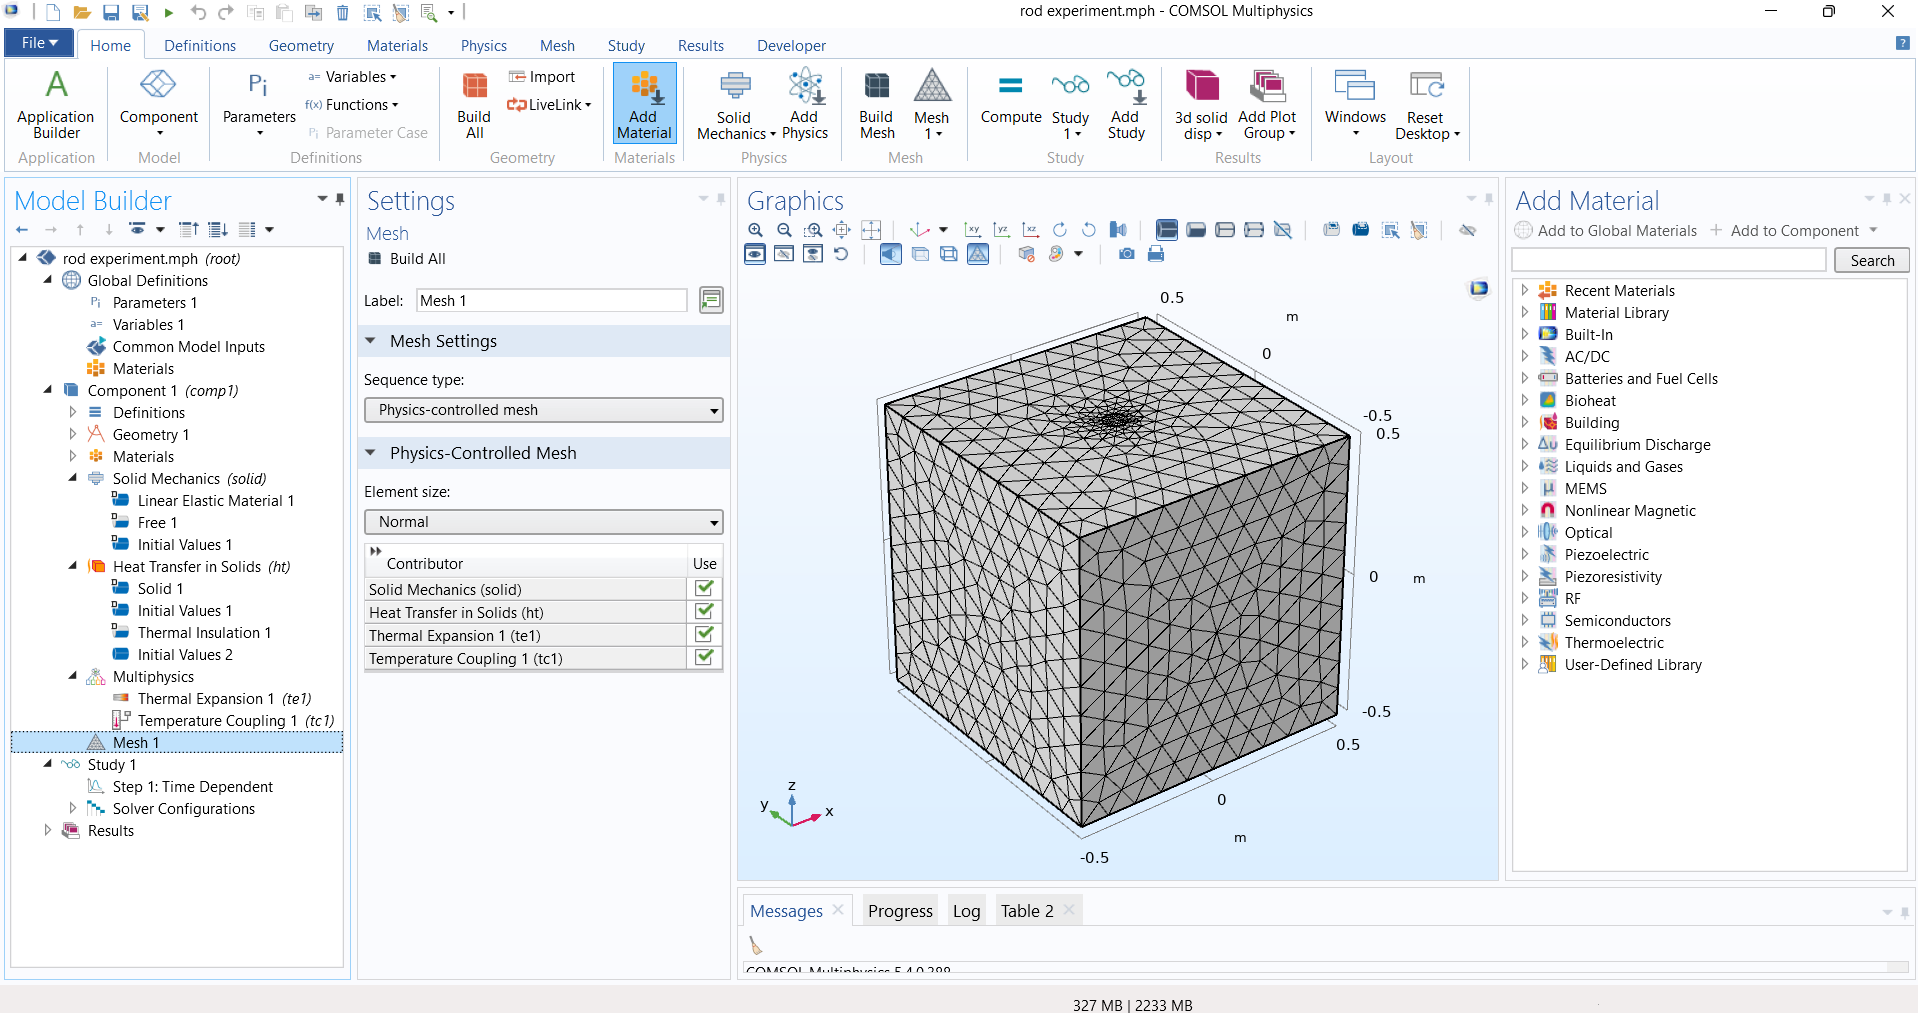
\includegraphics[width=0.8\textwidth]{chapters/chapter4/interface.png}
\caption{interface of Comsol Multiphysics}
\end{figure}

The simulated physical system consists of a two-dimensional rock domain and a heated metallic rod partially inserted into the rock. The rock represents the geological medium, while the rod acts as a localized thermal excitation source. The size of the rock domain is denoted as

\[
L_x \times L_y \times L_z.
\]

The radius of the inserted rod is denoted by

\[
R_{\mathrm{rod}},
\]

and the penetration depth of the rod into the rock is denoted by

\[
d_{\mathrm{rod}}.
\]

The initial temperature of the rock is denoted by \(T_0\), while the initial temperature of the rod is denoted by \(T_{\mathrm{rod}}\). In the considered experiment, the rod is hotter than the surrounding rock:

\[
T_{\mathrm{rod}} > T_0.
\]

The heated rod creates a localized temperature disturbance. Heat propagates from the rod into the surrounding geological medium by conduction. Since the temperature distribution inside the rock is non-uniform, different parts of the material expand by different amounts. This produces thermal strain, mechanical stress, and displacement fields. In a time-dependent formulation, the mechanical response appears as a propagating thermoelastic disturbance through the rock volume.

The computational domain is written as

\[
\Omega =
\Omega_{\mathrm{rock}}
\cup
\Omega_{\mathrm{rod}},
\]

where \(\Omega_{\mathrm{rock}}\) is the rock domain and \(\Omega_{\mathrm{rod}}\) is the rod domain. In COMSOL, these domains are assigned different material properties. This is important because the thermal and mechanical response of metal and rock are different.

\subsubsection{Physical interfaces used in COMSOL}

The COMSOL model was configured as a coupled thermo-mechanical simulation. The physical interfaces can be grouped into four main parts.

The first part is the thermal physics. The \textit{Heat Transfer in Solids} interface was used to solve transient heat conduction in both the rock and the rod. This interface computes the temperature field \(T(x,t)\) over the computational domain.

The second part is the structural mechanics. The \textit{Solid Mechanics} interface was used to compute displacement, strain, and stress caused by thermal expansion and dynamic mechanical response. The displacement field is obtained as a function of space and time.

The third part is the multiphysics coupling. The \textit{Thermal Expansion} coupling transfers the temperature field from the heat transfer interface to the solid mechanics interface. The temperature change produces thermal strain, which is included in the mechanical formulation.

The fourth part is the time-dependent study. The coupled system is solved over a time interval, producing a sequence of physical fields at multiple time steps. Therefore, the output of the COMSOL model is not a single static solution, but a time-dependent sequence of thermoelastic states.
\subsubsection{Heat transfer formulation}

The heat transfer process is based on Fourier's law:

\[
q = -k \nabla T,
\]

where \(q\) is the heat flux vector, \(k\) is the thermal conductivity, and \(T\) is the temperature field. The negative sign means that heat flows from hotter regions to colder regions. Therefore, the heat flux is directed opposite to the temperature gradient.

The transient heat conduction equation is written as

\[
\rho C_p \frac{\partial T}{\partial t}
=
\nabla \cdot \left( k \nabla T \right) + Q,
\]

where \(\rho\) is the material density, \(C_p\) is the heat capacity at constant pressure, \(t\) is time, and \(Q\) is the volumetric heat source. The left-hand side describes the accumulation of thermal energy inside the material. The first term on the right-hand side describes heat conduction, while \(Q\) represents internal or external heat generation.

In this experiment, the heated rod acts as the main source of thermal disturbance. Depending on the simulation setup, the rod can be represented either by an initial high temperature or by a prescribed heat source term. Since the rock and the rod are different materials, their thermal properties are spatially dependent:

\[
\rho = \rho(x), \qquad
C_p = C_p(x), \qquad
k = k(x),
\]

where

\[
x = (x, y).
\]

This means that the heat equation is solved with different material parameters in the rock and in the metallic rod.

\subsubsection{Solid mechanics formulation}

The mechanical response of the rock is described using the displacement vector

\[
u(x,t)
=
\begin{bmatrix}
u(x,t) \\
v(x,t) \\
w(x,t)
\end{bmatrix},
\]

where \(u\), \(v\), and \(w\) are displacement components along the \(x\), \(y\), and \(z\) axes. For small deformations, the strain tensor is defined as

\[
\varepsilon
=
\frac{1}{2}
\left(
\nabla u
+
(\nabla u)^{T}
\right).
\]

This tensor describes local deformation caused by mechanical displacement. In a thermoelastic problem, deformation is caused not only by mechanical loading, but also by temperature change. The thermal strain is expressed as

\[
\varepsilon_{\mathrm{th}}
=
\alpha
\left(
T - T_{\mathrm{ref}}
\right)
I,
\]

where \(\alpha\) is the coefficient of thermal expansion, \(T_{\mathrm{ref}}\) is the reference temperature, and \(I\) is the identity tensor. Thermal strain describes expansion or contraction of the material due to heating or cooling.

The elastic strain is the part of the total strain that contributes to mechanical stress:

\[
\varepsilon_{\mathrm{el}}
=
\varepsilon
-
\varepsilon_{\mathrm{th}}.
\]

The constitutive relation between stress and elastic strain is written as

\[
\sigma
=
C
:
\left(
\varepsilon
-
\varepsilon_{\mathrm{th}}
\right),
\]

where \(\sigma\) is the Cauchy stress tensor and \(C\) is the elasticity tensor. For an isotropic linear elastic material, this relation can be written as

\[
\sigma
=
\lambda \,
\mathrm{tr}
\left(
\varepsilon_{\mathrm{el}}
\right)
I
+
2 \mu
\varepsilon_{\mathrm{el}},
\]

where \(\lambda\) and \(\mu\) are Lamé parameters:

\[
\lambda =
\frac{E \nu}
{(1+\nu)(1-2\nu)},
\qquad
\mu =
\frac{E}{2(1+\nu)}.
\]

Here, \(E\) is Young's modulus and \(\nu\) is Poisson's ratio. Young's modulus defines the stiffness of the material, while Poisson's ratio describes lateral deformation under loading.

The dynamic mechanical response is governed by the equation of motion:

\[
\rho
\frac{\partial^2 u}{\partial t^2}
=
\nabla \cdot \sigma
+
f,
\]

where \(\rho\) is the density and \(f\) is the body force vector. This equation describes how stress gradients produce acceleration of the material. The divergence of the stress tensor acts as an internal force, while the inertial term controls wave-like propagation of displacement.

\subsubsection{Thermoelastic coupling}

The thermoelastic coupling is the central physical mechanism of the simulation. The heat transfer interface computes the temperature field \(T(x,t)\). This temperature field is then passed to the solid mechanics interface. COMSOL uses the temperature difference relative to the reference temperature to compute the thermal strain:

\[
\varepsilon_{\mathrm{th}}
=
\alpha
\left(
T - T_{\mathrm{ref}}
\right)
I.
\]

The thermal strain modifies the elastic strain. As a result, the stress tensor and displacement field change over time. The main physical chain of the experiment can be summarized as

\[
T(x,t)
\longrightarrow
\varepsilon_{\mathrm{th}}(x,t)
\longrightarrow
\sigma(x,t)
\longrightarrow
u(x,t).
\]

A more detailed chain can be written as

\[
T
\rightarrow
\nabla T
\rightarrow
\varepsilon_{\mathrm{th}}
\rightarrow
\sigma
\rightarrow
u
\rightarrow
\frac{\partial u}{\partial t}.
\]

This chain shows that the temperature field is not only a separate physical variable, but also the source of mechanical deformation and stress. Later, the neural network learns this coupled spatio-temporal relationship from the exported COMSOL data.
\subsubsection{Boundary and initial conditions}

The initial thermal conditions define the starting temperature contrast between the rod and the rock. For the rock domain,

\[
T(x,0) = T_0,
\qquad
x \in \Omega_{\mathrm{rock}},
\]

and for the rod domain,

\[
T(x,0) = T_{\mathrm{rod}},
\qquad
x \in \Omega_{\mathrm{rod}}.
\]

Since

\[
T_{\mathrm{rod}} > T_0,
\]

an initial thermal contrast is created at the contact region between the rod and the rock. This contrast is the main reason for heat propagation into the geological medium.

For thermally insulated boundaries, the heat flux through the selected external surfaces is set to zero:

\[
-n \cdot q = 0,
\]

or, using Fourier's law,

\[
n \cdot k \nabla T = 0,
\]

where \(n\) is the outward normal vector to the boundary. This boundary condition means that no heat leaves the model through the selected external surfaces. It is useful when the goal is to study internal heat propagation inside the geological volume.

If external cooling is included in a specific scenario, a convection boundary condition can be used:

\[
-n \cdot q
=
h
\left(
T - T_{\mathrm{ext}}
\right),
\]

where \(h\) is the heat transfer coefficient and \(T_{\mathrm{ext}}\) is the external ambient temperature. In this work, this condition can be considered as an optional boundary condition depending on the selected simulation scenario.

Mechanical boundary conditions are required to keep the structural problem stable and physically meaningful. A fixed boundary can be defined as

\[
u = 0
\quad
\text{on}
\quad
\Gamma_{\mathrm{fixed}}.
\]

This condition prevents rigid body motion of the entire computational domain. A free surface boundary can be written as

\[
\sigma\,n = 0
\quad
\text{on}
\quad
\Gamma_{\mathrm{free}}.
\]

This condition allows natural deformation of external surfaces without applying additional external traction. The choice of mechanical boundary conditions affects wave reflections and stress distribution. Therefore, during dataset generation, the boundary conditions must be kept consistent across simulations. This ensures that the neural network learns differences caused by material and source parameters rather than changes in the numerical setup.

\subsubsection{Material parameters}

The material definition is one of the most important parts of the COMSOL simulation. The rock and the rod must be assigned thermal and mechanical properties. These properties determine how quickly heat propagates, how strongly the material expands, and how mechanical waves travel through the medium.

\begin{table}[h]
\centering
\caption{Main material parameters used in the thermoelastic COMSOL simulation.}
\label{tab:comsol_material_parameters}
\begin{tabular}{lll}
\hline
Parameter & Symbol & Physical meaning \\
\hline
Density & \(\rho\) & Controls inertia and heat capacity per unit volume \\
Thermal conductivity & \(k\) & Controls the rate of heat diffusion \\
Heat capacity & \(C_p\) & Controls thermal energy storage \\
Young's modulus & \(E\) & Defines material stiffness \\
Poisson's ratio & \(\nu\) & Defines lateral deformation under loading \\
Thermal expansion coefficient & \(\alpha\) & Couples temperature change with strain \\
\hline
\end{tabular}
\end{table}

The parameters \(k\) and \(C_p\) determine how quickly the temperature field changes. A material with high thermal conductivity transfers heat faster, while a material with high heat capacity requires more energy to change its temperature. The parameters \(E\) and \(\nu\) determine the mechanical stiffness and deformation behavior of the material. The coefficient \(\alpha\) links temperature variation with mechanical deformation. Density \(\rho\) influences both thermal energy storage and dynamic wave propagation.

No fixed numerical values are introduced in this subsection because the material parameters may vary between simulation scenarios. This allows the same COMSOL setup to be used for different rock types and different thermal excitation conditions.

\subsubsection{Finite element mesh generation}

COMSOL uses finite element discretization to solve the coupled thermo-mechanical problem. The continuous computational domain is divided into finite elements, and the solution is computed at mesh nodes or interpolation points. The discretized domain can be written as

\[
\Omega_h =
\bigcup_{e=1}^{N_e}
\Omega_e,
\]

where \(\Omega\) is the continuous computational domain, \(\Omega_h\) is the discretized finite element domain, \(\Omega_e\) is a finite element, and \(N_e\) is the number of elements.

A finer mesh is required near the heated rod because temperature gradients and stress gradients are stronger in this region. If the mesh is too coarse near the rod, the simulation may not accurately capture the local thermal contrast and the corresponding stress concentration. At the same time, a very fine mesh over the entire volume increases computational cost. Therefore, the mesh should be refined mainly in physically important regions.

The finite element mesh is also important for the machine learning stage. Each mesh node can be interpreted as a graph node, while connections between neighboring nodes or elements can be interpreted as graph edges. Therefore, the COMSOL mesh provides not only numerical discretization for FEM, but also a natural spatial structure for graph-based neural networks.

The graph representation can be written as

\[
\mathcal{G} = (\mathcal{V}, \mathcal{E}),
\]

where \(\mathcal{V}\) is the set of graph nodes and \(\mathcal{E}\) is the set of graph edges. For each node,

\[
x_i =
(x_i, y_i),
\qquad
i = 1,2,\dots,N,
\]

where \(x_i\) are node coordinates. For each edge between neighboring nodes \(i\) and \(j\), edge attributes can be defined as

\[
e_{ij}
=
\left[
x_j - x_i,
\;
\left\|
x_j - x_i
\right\|
\right].
\]

These edge attributes describe the relative position and distance between neighboring nodes. This representation is especially important for MeshGraphNet because the model uses local message passing between connected nodes.

\subsubsection{Time-dependent simulation}

The thermoelastic simulation is performed over the time interval

\[
t \in [0, t_{\max}].
\]

The discrete time steps are defined as

\[
t_n = n \Delta t,
\qquad
n = 0,1,\dots,N_t.
\]

At each time step, COMSOL computes the main thermal and mechanical fields:

\[
T(x,t_n),
\qquad
u(x,t_n),
\qquad
\sigma(x,t_n),
\qquad
\varepsilon(x,t_n).
\]

The result is not a single static field, but a sequence of physical states. This sequence forms the basis of the spatio-temporal dataset. For neural network training, the time-dependent simulation can be interpreted as a mapping from the current physical state to the next state:

\[
\mathcal{F}_{\Delta t}:
s(t_n)
\rightarrow
s(t_{n+1}).
\]

For a longer prediction horizon, the mapping can be written as

\[
\mathcal{F}_{m\Delta t}:
s(t_n)
\rightarrow
s(t_{n+m}).
\]

For a mesh node \(i\), the physical state vector may include temperature, displacement, velocity, and stress components:

\[
s_i(t)
=
\left[
T_i(t),
u_i(t),
v_i(t),
\dot{u}_i(t),
\dot{v}_i(t),
\sigma_{x,i}(t),
\sigma_{y,i}(t),
\sigma_{xy,i}(t)
\right].
\]

Here, \(i\) denotes a mesh node. This formulation is suitable for machine learning because every simulation produces a sequence of states with the same physical meaning.
\subsubsection{Exported simulation fields}

The COMSOL simulation exports the physical fields required for training and validating AI models. Because the formulation in this thesis is two-dimensional under the plane-strain assumption, only the in-plane components are retained for the dataset. The exported variables include thermal variables, mechanical variables, and material parameters. The thermal variables include temperature \(T\), thermal conductivity \(k\), density \(\rho\), and heat capacity \(C_p\). The mechanical variables include in-plane displacement components \(u\) and \(v\), in-plane velocity components \(u_t\) and \(v_t\), von Mises stress \(\sigma_{\mathrm{vM}}\), in-plane stress tensor components \(\sigma_x\), \(\sigma_y\), \(\sigma_{xy}\), and in-plane strain components \(\varepsilon_x\), \(\varepsilon_y\), \(\varepsilon_{xy}\). The material parameters include Young's modulus \(E\), Poisson's ratio \(\nu\), solid density \(\rho_s\), and thermal expansion coefficient \(\alpha\).

\begin{table}[h]
\centering
\caption{Main exported variables from the COMSOL thermoelastic simulation.}
\label{tab:comsol_exported_variables}
\begin{tabular}{lll}
\hline
Group & Variables & Description \\
\hline
Thermal field & \(T\) & Temperature distribution \\
Thermal properties & \(k\), \(\rho\), \(C_p\) & Heat transfer material parameters \\
Displacement & \(u\), \(v\) & In-plane mechanical displacement components \\
Velocity & \(u_t\), \(v_t\) & Time derivatives of in-plane displacement components \\
Stress & \(\sigma_{\mathrm{vM}}\), \(\sigma_x\), \(\sigma_y\), \(\sigma_{xy}\) & In-plane stress field components \\
Strain & \(\varepsilon_x\), \(\varepsilon_y\), \(\varepsilon_{xy}\) & In-plane strain field components \\
Material properties & \(E\), \(\nu\), \(\rho_s\), \(\alpha\) & Elastic and thermoelastic parameters \\
\hline
\end{tabular}
\end{table}

In addition to physical fields, mesh-related arrays can be stored separately. These include node coordinates, mesh connectivity, edge attributes, time vector, and normalization statistics. The node feature matrix for one time step can be represented as

\[
X
\in
\mathbb{R}^{N \times F},
\]

where \(N\) is the number of mesh nodes and \(F\) is the number of node features. For time-dependent data, the tensor form is

\[
X
\in
\mathbb{R}^{N_t \times N \times F}.
\]

This format stores feature values for every time step, every mesh node, and every physical channel. It is convenient because the same simulation output can later be transformed into graph-based, grid-based, or sequence-based datasets.

\subsubsection{Relation to machine learning dataset generation}

COMSOL acts as the source of ground-truth data. During inference, the neural network does not directly solve the heat transfer equation or the solid mechanics equation. Instead, it learns an approximation of the solution operator from examples generated by COMSOL.

The general operator can be written as

\[
\mathcal{G}:
\left(
s(t),
p,
x
\right)
\mapsto
s(t+\Delta t),
\]

where \(s(t)\) is the current physical state, \(p\) contains material and source parameters, \(x\) denotes spatial coordinates, and \(s(t+\Delta t)\) is the future physical state.

For MeshGraphNet, the prediction for node \(i\) can be written as

\[
\hat{s}_i(t+\Delta t)
=
f_{\theta}
\left(
s_i(t),
x_i,
p_i,
\left\{
s_j(t), e_{ij}
\right\}_{j \in \mathcal{N}(i)}
\right),
\]

where \(f_{\theta}\) is the neural network model, \(\mathcal{N}(i)\) is the set of neighboring nodes of node \(i\), and \(e_{ij}\) are edge features. This formulation is consistent with MeshGraphNet because physical processes in a solid medium are local: the future state of a node depends on its own state, material parameters, and neighboring nodes.

The same COMSOL data can also be transformed for other models. For FNO, the exported fields can be interpolated or represented on a regular grid. For PINN, the simulation data can be used together with physical residuals and collocation points. For Transformer-based models, the exported time series can be represented as temporal sequences. The detailed description of these models is outside this subsection and is provided in the AI models section.

\subsubsection{Visualization of the simulation results}

COMSOL was also used for visual inspection of the simulation results. Visualization is important because numerical fields must be checked not only by exported values, but also by their physical behavior. The geometry, mesh, temperature distribution, displacement field, stress field, and wave-like propagation were inspected during the simulation process.

Figure~\ref{fig:comsol_geometry} shows the geometry of the rock domain with the inserted heated rod. This figure is useful for demonstrating the physical setup of the experiment.

\begin{figure}[h]
\centering
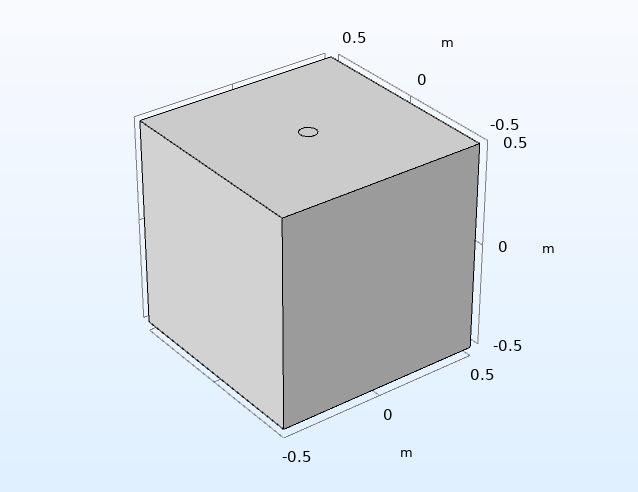
\includegraphics[width=0.8\textwidth]{chapters/chapter4/object.png}
\caption{Geometry of the rock domain with the inserted heated rod.}
\label{fig:comsol_geometry}
\end{figure}

Figure~\ref{fig:comsol_mesh} illustrates the finite element mesh used for solving the coupled thermoelastic problem. The mesh defines both the numerical discretization and the spatial structure later used in graph-based machine learning.

\begin{figure}[h]
\centering
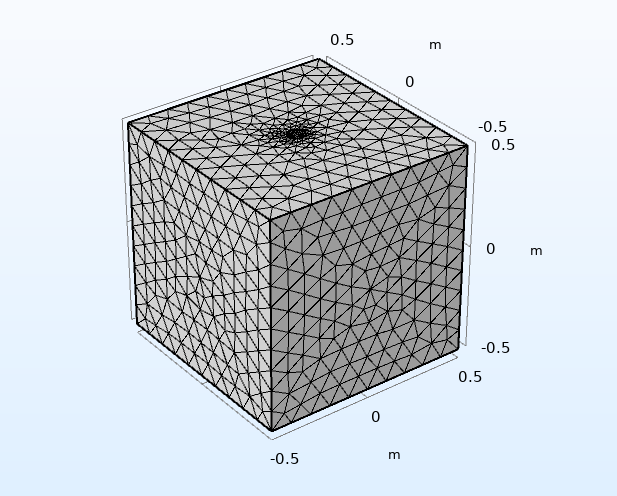
\includegraphics[width=0.8\textwidth]{chapters/chapter4/mesh.png}
\caption{Finite element mesh used for the thermoelastic COMSOL simulation.}
\label{fig:comsol_mesh}
\end{figure}

Figure~\ref{fig:comsol_temperature} shows the temperature distribution produced by the heated rod. This visualization allows checking whether heat propagates from the source into the surrounding rock in a physically reasonable way.

\begin{figure}[h]
\centering
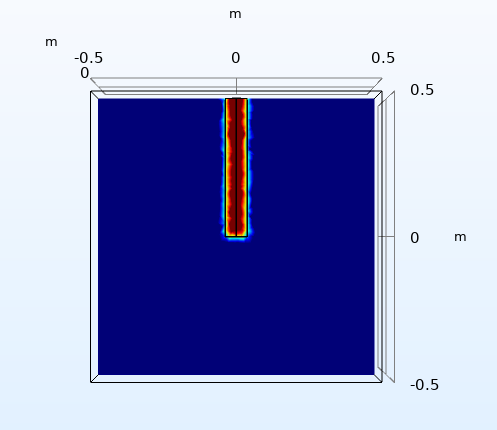
\includegraphics[width=0.8\textwidth]{chapters/chapter4/temperature.png}
\caption{Temperature distribution in the rock caused by the heated rod.}
\label{fig:comsol_temperature}
\end{figure}

Figure~\ref{fig:comsol_stress} shows the stress field generated by non-uniform thermal expansion. This field is important because it represents the mechanical response of the geological medium to the thermal disturbance.

\begin{figure}[H]
    \centering

    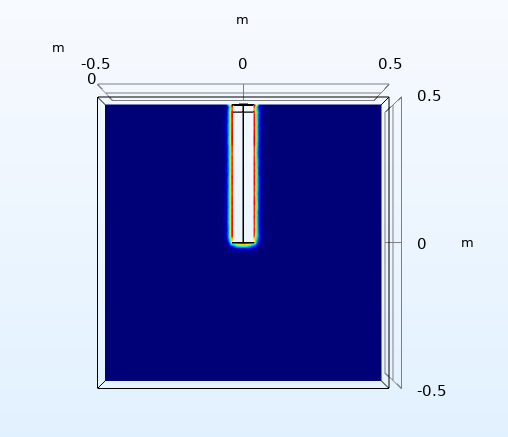
\includegraphics[width=0.8\textwidth]{chapters/chapter4/stress_1.png}

    \vspace{0.3cm}

    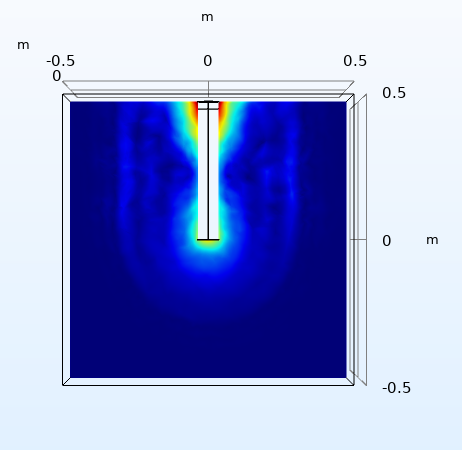
\includegraphics[width=0.8\textwidth]{chapters/chapter4/stress_2.png}

    \vspace{0.3cm}

    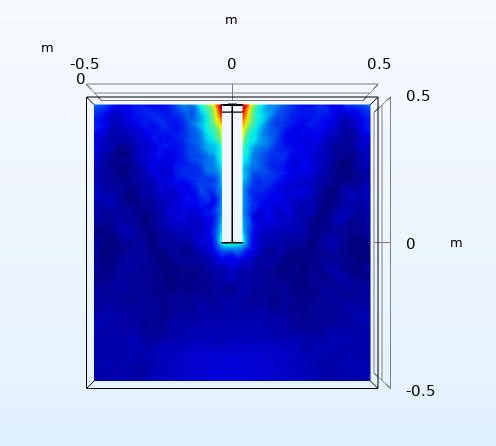
\includegraphics[width=0.8\textwidth]{chapters/chapter4/stress_3.png}

    \caption{Evolution of the stress field in the rock at three time
    instants (top: beginning of the heating; middle: intermediate
    state; bottom: end of the simulated interval). Non-uniform thermal
    expansion produces stress concentrations in the heated zone and
    along the rod--rock interface.}
    \label{fig:comsol_stress}
\end{figure}


\subsubsection{Limitations of the simulation setup}

The quality of synthetic data depends on the geometry, material parameters, boundary conditions, mesh resolution, and solver settings. If the geometry is too simplified, the generated data may not fully represent real geological formations. If the material model assumes homogeneous and isotropic rock, it may differ from real rocks, which can contain cracks, layers, pores, and anisotropic properties.

Mesh resolution also affects numerical accuracy. A coarse mesh may not capture sharp temperature gradients near the rod or stress concentration zones. A very fine mesh improves accuracy, but increases computational cost. Similarly, the selected time step \(\Delta t\) affects stability and accuracy of the time-dependent solution.

Limited computational resources restricted the complexity and number of simulated scenarios. For example, very large two-dimensional models, very fine meshes, and many parameter combinations require significant memory and computation time. However, these limitations were controlled by keeping the setup consistent and by focusing on physically meaningful scenarios.

Despite these limitations, controlled synthetic generation is suitable for training and comparing AI models because all required physical fields are available and consistently exported. This is a major advantage compared to real experimental data, where some fields may be difficult or impossible to measure directly.
\subsection{Summary of Chapter 4}

This chapter described the COMSOL Multiphysics simulation used to generate a controlled synthetic dataset for thermoelastic wave propagation in geological media. The simulation represented a two-dimensional rock domain with a heated rod acting as a localized thermal source. The resulting temperature contrast produced heat conduction, thermal expansion, stress formation, displacement, and wave-like mechanical response.

The chapter also explained how the raw COMSOL outputs were converted into a machine-learning-ready dataset. Temperature, displacement, velocity, stress, strain, material parameters, coordinates, and mesh information were exported, cleaned, aligned, normalized, and stored in a common structure suitable for different surrogate models. The limitations of this setup were stated explicitly: the dataset is synthetic, mesh- and time-step-dependent, and represents an idealized two-dimensional scenario rather than a direct field measurement.


\clearpage

%Chapter 5.
\section{Implementation and System Architecture}

\subsection{Implementation and System Architecture}

This section describes the software implementation used to realize the prediction methodology introduced in Chapter~4. The purpose of the implementation is not to reproduce a full industrial geophysical simulator, but to provide a research prototype in which several predictive model families can be compared under one physically motivated workflow. In this sense, the system connects user-defined thermoelastic scenarios, effective geological material parameters, model routing, and normalized prediction summaries into one reproducible experimental stack. The implementation therefore acts as the practical bridge between the geological motivation of Chapter~2, the thermoelastic variables and governing relations of Chapter~3, and the comparative prediction task formulated in Chapter~4.

At the architectural level, the implementation is organized as a service-oriented prototype. The full local stack is composed of a backend orchestrator, a web-based scientific frontend, a set of independent model services, a structured catalog of geological media, and a container-based local orchestration layer. In practical terms, the system can be understood as a pipeline in which the user configures a geological medium and a thermoelastic scenario in the frontend, the backend validates and enriches the request, the selected model service performs the prediction, and the normalized response is returned for display, comparison, and summary reporting. This design is appropriate for the thesis because the main scientific question is comparative directional prediction rather than monolithic solver construction.

The frontend is the user-facing layer of the prototype. Its role is to provide a compact scientific interface for selecting a geological medium, choosing a prediction route, specifying the source and probe geometry, defining thermal and mechanical conditions, and visualizing the returned prediction summary. The frontend dynamically loads media and model information from the backend and presents a two-dimensional domain view for interactive experiments. From the perspective of the thesis, the frontend should therefore be described as an experimental configuration and visualization surface rather than as a source of physical modelling. It does not perform the thermoelastic computation itself. Instead, it exposes the structured inputs needed by the prediction workflow and displays the resulting directional quantities and field-level summary indicators.

The backend is the central orchestration layer of the system. This distinction is important: the backend is not the machine-learning model itself. It validates a unified prediction request, resolves the geological medium from the catalog, merges scenario inputs with rock presets, routes the request to the selected remote model service, and normalizes the response before returning it to the caller. The unified request structure carries the selected model, a medium identifier, scenario parameters, source coordinates and direction, probe coordinates, and a domain description. The backend also validates geometric consistency, for example by requiring that the out-of-plane size and resolution collapse to a single planar slice for two-dimensional cases. As a result, the backend provides the common contract that allows different model services to be compared under the same physical input description.

The geological medium catalog is a compact repository of effective material presets. It includes media such as sandstone, limestone, basalt, and granite together with representative properties such as density, total and effective porosity, \(V_p\), \(V_s\), thermal conductivity, heat capacity, and thermal expansion. These entries are not full geological databases and should not be interpreted as field-validated constitutive models. Instead, they serve the thesis purpose of supplying effective material parameters for locally homogeneous and isotropic thermoelastic modelling. This is fully consistent with the simplifications introduced in Chapters~2 and~3, where real geological media are recognized as heterogeneous, porous, fractured, layered, and often anisotropic, but the mathematical formulation proceeds through effective continuum parameters.

The predictive components are separated into distinct services. This separation is useful because it makes the comparison framework explicit and prevents the backend from being mistaken for a single model implementation. The PINN component is the closest to the governing equations of Chapter~3. It predicts the primary fields \((T, u, v)\) and is trained with a combination of a supervised loss, a velocity consistency term, an elastic wave residual, and a coupled thermal residual. The residual terms are built from the thermoelastic stress tensor, displacement gradients, and the coupled heat equation with the \(\gamma T_0 \, \partial \varepsilon_{kk}/\partial t\) term. For this reason, the PINN is the only explicitly physics-informed baseline in the current comparison.

The FNO component is implemented as a dedicated Fourier Neural Operator route and is configured as a trainable two-dimensional baseline. Its current purpose is to learn the evolution of physically meaningful fields on a regular grid, with targets such as temperature and displacement components. Its training objective is a supervised loss of the form
\begin{equation}
\mathcal{L}_{\mathrm{FNO}}
=
\operatorname{MSE}(\widehat{Y},Y)
+ 0.01 \, \operatorname{relativeL2}(\widehat{Y},Y),
\end{equation}
without explicit thermoelastic PDE residual enforcement. It is therefore described in the thesis as a neural-operator baseline rather than as a physics-constrained solver. This distinction matters because the model still operates on physically meaningful fields, yet it does not incorporate the governing thermoelastic equations in the same way as the PINN.

The MeshGraphNet component provides the graph-based route. It can run a MeshGraphNet-style rollout when dataset and checkpoint artifacts are configured, and it can also return a deterministic fallback response when these artifacts are unavailable and fallback is enabled. This means that the component is best described as a graph-based predictive route within a prototype architecture. It is relevant to the thesis because directional propagation in geological media is naturally linked to geometry, local neighborhoods, and mesh-like spatial relationships. At the same time, its practical interpretation must remain careful: depending on the run configuration, the returned result may reflect either a learned graph-based prediction or fallback logic intended to keep the system operational for demonstration and interface testing.

The Transformer-style component is an autoregressive neural-operator baseline parallel to the PINN. Its architecture uses tokens carrying coordinates, current-state fields, and material properties, and predicts \((T, u, v)\) at target coordinates. The current version uses a supervised data loss only and does not yet include physics-informed residuals. It is therefore described in the thesis as an experimental supervised sequence/operator-style baseline whose maturity is lower than that of the main orchestration pattern.

Taken together, these components form a common comparative architecture rather than four physically equivalent solvers. All of them receive inputs motivated by the same thermoelastic problem definition, but they use the physics differently. The PINN is the only component whose training objective explicitly contains thermoelastic residuals derived from the governing equations. The FNO, MeshGraphNet, and Transformer-style routes use physically meaningful inputs and outputs, but they do not enforce the full coupled thermoelastic PDE system in the same way. This wording is important for consistency with Chapter~4 and for avoiding overstatement in the thesis.

Both the mathematical formulation in Chapter~3 and the prototype implementation are two-dimensional. The current experiments operate on planar source--probe paths and two-dimensional cross-sections that are practical for the available data and prototype model components. In such settings, source and probe positions are selected within a single plane, and the directional response is described entirely by the in-plane geometry introduced in Chapter~3.

The deployment structure of the project reinforces this interpretation. The container-based local environment starts the frontend, the backend, and each model component as a separate service with its own health or readiness endpoint. This design is valuable for a bachelor-level research prototype because it isolates component responsibilities, makes failure modes more visible, and allows individual components to be replaced or upgraded without rewriting the entire stack. The project also provides component-specific scripts and procedures for data preparation, training, checkpoint management, validation, and local startup. These support reproducibility and experimentation, even though they do not by themselves establish scientific validation.

In summary, Chapter~6 implements the methodology of Chapter~4 through a backend-centered orchestration stack that connects user inputs, effective geological material presets, model routing, and normalized directional prediction outputs. The implementation should be described as a comparative research prototype with physics-informed and data-driven components, not as a final validated two-dimensional thermoelastic simulator. Its main strengths are unified routing, explicit material handling, component modularity, and transparent model comparison. Its main limitations are equally important: the prototype is two-dimensional, medium presets remain starter values, different model routes use physics at different depths, and fallback-capable components must be interpreted carefully when reporting comparative results.

\subsection{Prediction API Contract}

The practical comparison of several predictive model services requires a unified input-output contract. Without such a contract, each model route would expose its own ad hoc request structure, making scientific comparison difficult and implementation fragile. In the present thesis, the API contract serves as the operational link between the thermoelastic variables introduced in Chapter~2 and the prediction task formulation introduced in Chapter~3. It ensures that different model services receive the same physical scenario description, that responses can be normalized into a common format, and that the resulting outputs can be compared in a single experimental workflow.

At the request level, the backend schema groups the prediction inputs into several logically distinct parts. The first group is model selection, represented by the field \texttt{model}. This field identifies the route to be used, such as \texttt{pinn}, \texttt{fno}, \texttt{meshgraphnet}, or an experimental Transformer-style route. The second group is material identification, represented in the current backend by a medium identifier such as \texttt{medium\_id}. Rather than requiring the user to enter every physical constant manually for each experiment, the system can resolve the material from the geological catalog and enrich the prediction request with the corresponding preset properties. This design keeps the public interface compact while preserving a physical interpretation of the selected medium.

The material-related part of the contract is conceptually grounded in the parameters already defined in Chapter~2. These include the material name or medium type together with effective quantities such as density \(\rho\), Young's modulus \(E\), Poisson's ratio \(\nu\), shear modulus \(\mu\), bulk modulus \(K\), Lam\'e parameter \(\lambda\), thermal expansion coefficient \(\alpha\), thermal conductivity \(k\), specific heat capacity \(C_p\), volumetric heat capacity \(C=\rho C_p\), thermoelastic coupling coefficient \(\gamma=3K\alpha\), and, where available, wave velocities \(V_p\) and \(V_s\) and porosity. In the current repository, the public backend request does not require all of these values to be typed explicitly. Instead, the catalog stores a practical subset, including \(\rho\), porosity, \(V_p\), \(V_s\), thermal conductivity, heat capacity, and thermal expansion, while other effective quantities may be derived internally or supplied through model-specific datasets. For the thesis, this should be described as a physically motivated material contract rather than as a claim that every route consumes the entire constitutive parameter set in identical form.

The next input group describes the thermoelastic scenario. In the current backend schema this role is played by the \texttt{scenario} object, which includes at least \texttt{temperature\_c}, \texttt{pressure\_mpa}, and \texttt{time\_ms}. These parameters encode the thermal and mechanical state under which the prediction is requested. The source object adds the excitation description through fields such as source type, source coordinates, amplitude, frequency, and a direction vector. The probe object specifies the observation point. Together, these fields provide the practical representation of the source--probe geometry introduced theoretically in Chapter~2.

The directional part of the contract follows directly from the mathematical formulation. If the source position is denoted by \(\mathbf{x}_s\) and the probe position by \(\mathbf{x}_p\), then the propagation vector is
\begin{equation}
\mathbf{d}
=
\mathbf{x}_p - \mathbf{x}_s,
\end{equation}
and the corresponding unit direction vector is
\begin{equation}
\hat{\mathbf{d}}
=
\frac{\mathbf{d}}{\|\mathbf{d}\|}.
\end{equation}
From this vector, directional quantities such as propagation distance, azimuth, and elevation can be computed. In three-dimensional notation, if \(\mathbf{d}=(d_x,d_y,d_z)\), then the azimuth is given by
\begin{equation}
\phi = \operatorname{atan2}(d_y,d_x),
\end{equation}
and the elevation is given by
\begin{equation}
\psi =
\operatorname{atan2}
\left(
d_z,\sqrt{d_x^2+d_y^2}
\right).
\end{equation}
The backend request schema additionally validates the user-provided source direction to ensure that it is finite and nonzero before normalization. This is important because the source direction may later be compared with the source--probe direction or combined with geometry-aware post-processing in model-specific inference pipelines.

Another required input group is the domain description. In the current backend, this is represented by the \texttt{domain} object with subfields such as \texttt{type}, \texttt{size}, \texttt{resolution}, and boundary conditions. At the theoretical level, Chapter~2 is formulated in general three-dimensional form, so a general contract may allow both \texttt{rect\_2d} and \texttt{rect\_3d}. However, the practical thesis experiments are prototype experiments and are primarily based on \texttt{rect\_2d} domains. The backend validator explicitly requires \texttt{lz = 0} and \texttt{nz = 1} when \texttt{domain.type = rect\_2d}. This is a useful implementation detail because it encodes the practical scope directly in the API contract: the general request shape remains compatible with future three-dimensional extensions, but the current experiments operate on planar cross-sections or selected directional paths.

The output side of the contract is designed to provide one normalized summary format across different services. According to the backend response schema and repository model card, the normalized prediction response contains a selected model identifier, a medium summary, directional prediction quantities, field-summary quantities, and technical metadata. The directional summary includes a direction vector, azimuth, elevation, response magnitude, wave type, and predicted travel time. The field summary includes at least maximum displacement and maximum temperature perturbation. The metadata block includes items such as model version, latency, and request identifier. These outputs correspond naturally to the comparative prediction goal of the thesis because they summarize directional thermoelastic behavior without requiring every model route to expose the same internal field representation.

It is important to distinguish between primary public outputs and internal physical diagnostics. In the current API, stress and strain are not the main direct outputs of the normalized response. This is consistent with the practical role of the system, which compares directional summary quantities and field-level indicators rather than exposing a full continuum-mechanics state tensor in every response. Nevertheless, stress and strain remain physically meaningful variables from Chapter~2. In the PINN route they are used internally for residual computation, and in principle they can also be derived as diagnostics from predicted displacement and temperature fields when sufficiently rich spatial information is available. For the thesis, it is therefore correct to say that the present API is centered on temperature-related and displacement-related response quantities, while stress and strain are treated primarily as internal or derived quantities rather than standard public outputs for all model services.

The following illustrative structure shows the spirit of the unified request contract in a compact form:

\begin{verbatim}
{
  "model": "pinn",
  "medium_id": "basalt",
  "scenario": {
    "temperature_c": 100,
    "pressure_mpa": 10,
    "time_ms": 5
  },
  "domain": {
    "type": "rect_2d",
    "size": {"lx": 1.0, "ly": 1.0, "lz": 0.0},
    "resolution": {"nx": 128, "ny": 128, "nz": 1}
  },
  "source": {
    "type": "thermal_pulse",
    "x": 0.2, "y": 0.5, "z": 0.0,
    "amplitude": 1.0,
    "frequency_hz": 50,
    "direction": [1.0, 0.0, 0.0]
  },
  "probe": {"x": 0.8, "y": 0.5, "z": 0.0}
}
\end{verbatim}

An illustrative normalized or experiment-summary response may be written as follows:

\begin{verbatim}
{
  "model": "pinn",
  "status": "ok",
  "travel_time_ms_pred": 1.25,
  "max_displacement": 0.00012,
  "max_temperature_perturbation": 15.3,
  "magnitude": 0.82,
  "azimuth_deg": 0.0,
  "elevation_deg": 0.0,
  "effective_domain_type": "rect_2d",
  "fallback_used": false
}
\end{verbatim}

These examples are illustrative rather than normative, but they show the intended logic of the contract. The scientific fields are grouped separately from technical execution metadata. This is especially important in a prototype comparison system. For honest reporting, experimental summary tables should preserve not only the scientific outputs, but also route-level technical indicators such as execution status, fallback usage, and error messages when present. Such fields do not make the prediction more physical, but they are essential for reproducibility and for distinguishing learned predictions from placeholder or degraded execution paths.

The unified contract also clarifies how the models should be compared. All routes should be evaluated on the same 2D input cases, with the same material preset, source--probe geometry, and scenario parameters. Their outputs should then be stored in a common summary table or experiment log so that travel time, direction, displacement-related response, and thermal response can be compared consistently. This is methodologically important because the contract standardizes the observable prediction task even when the internal model architectures differ substantially.

At the same time, the contract does not imply physical equivalence of the models. A common interface is not the same as a common solver. The PINN is the only explicitly physics-informed component in the present comparison because it includes thermoelastic residuals derived from the governing equations. The FNO, MeshGraphNet, and Transformer-style services use physically meaningful inputs and outputs, but they do not enforce the governing thermoelastic PDE system in the same way. The API contract therefore supports comparative experimentation under one physically motivated input-output framework, while preserving the important distinction between physics-informed and primarily data-driven routes.

The limitations of this contract follow naturally from the limitations of the prototype itself. The contract standardizes communication and comparison, but it does not guarantee validated field realism. The public outputs are comparative prototype predictions, not engineering-grade measurements. Material presets in the current repository are starter values. Some services may operate in fallback mode under missing-artifact conditions. The practical experiments are predominantly \texttt{rect\_2d} and should not be described as full three-dimensional field simulations. For these reasons, the API contract should be presented in the thesis as a disciplined experimental interface that supports fair comparison and reproducible software behavior, while remaining subordinate to the more general physical formulation of Chapter~2.

% \input{chapters/chapter5/experimental_2d_setup.tex}

\let\originalsection\section
\let\originalsubsection\subsection
\let\originalsubsubsection\subsubsection
\let\section\originalsubsection
\let\subsection\originalsubsubsection
\let\subsubsection\originalsubsubsection
\section{Physics-Informed Neural Network for Thermoelastic Prediction}

\subsection{Motivation for a physics-informed surrogate}

Among the four predictive routes considered in this thesis, the
physics-informed neural network (PINN) is the only one whose training
objective explicitly contains residuals of the governing thermoelastic
equations introduced in Chapter~3. The other three routes (FNO,
MeshGraphNet and the Transformer-style operator) are data-driven
surrogates: they are trained against simulation snapshots, but they do
not directly penalise violations of the coupled heat--momentum system.
The PINN component therefore plays a dual role inside the comparison
framework: it is both a candidate predictor and the only baseline that
embeds physical knowledge inside the loss.

\subsection{Network mapping and inputs}

The PINN is a single multilayer perceptron $f_{\theta}$ that takes a
point query in space--time together with the local material parameters
and returns the predicted thermoelastic state at that point:
\begin{equation}
f_{\theta}\colon\; 
\bigl(x,\,y,\,t,\,E,\,\nu,\,\rho,\,\alpha,\,k,\,C_p\bigr)
\;\longmapsto\;
\bigl(T,\,u,\,v\bigr).
\end{equation}
Here $(x,y)$ is the in-plane probe coordinate in the 2D plane-strain
domain, $t$ is the observation time, and the six material parameters
follow Section~3.4. The output triple $(T,u,v)$ contains the
temperature and the two in-plane displacement components; stress and
strain are recovered analytically from the predicted displacement and
temperature during loss assembly.

The network is implemented as an MLP with $L$ hidden layers of width
$d_h$ and a smooth activation $\varphi$ (the implementation uses
$\tanh$). Layer $\ell$ computes
\begin{equation}
h^{(\ell)} = \varphi\bigl(W^{(\ell)} h^{(\ell-1)} + b^{(\ell)}\bigr),
\qquad
h^{(0)} = z = (x,y,t,E,\nu,\rho,\alpha,k,C_p),
\end{equation}
and the output head produces
$(T,u,v) = W^{(L+1)} h^{(L)} + b^{(L+1)}$.
The smooth activation matters: $\tanh$ has bounded derivatives of
every order, so the higher-order derivatives needed by the PDE loss
(below) remain numerically stable.

\subsection{Composite training loss}

The PINN parameters $\theta$ are obtained by minimising a weighted sum
of four loss components on a batch of collocation points
$\{(x_i, y_i, t_i)\}$ drawn from the training scenarios:
\begin{equation}
\mathcal{L}(\theta)
=
\lambda_{\mathrm{sup}}\,\mathcal{L}_{\mathrm{sup}}
+ \lambda_{\mathrm{vel}}\,\mathcal{L}_{\mathrm{vel}}
+ \lambda_{\mathrm{el}}\,\mathcal{L}_{\mathrm{elastic}}
+ \lambda_{\mathrm{th}}\,\mathcal{L}_{\mathrm{thermal}}.
\end{equation}
The implementation-level assembly of this composite objective is shown
in Appendix~\ref{app:pinn-loss}.

Supervised loss $\mathcal{L}_{\mathrm{sup}}$ is the standard
mean-squared error between the predicted $(T,u,v)$ and the
ground-truth values exported from COMSOL at the corresponding
$(x_i,y_i,t_i)$.

Velocity consistency $\mathcal{L}_{\mathrm{vel}}$ enforces
that the displacement time derivative obtained by automatic
differentiation matches the velocity field that COMSOL reported as
$u_t,v_t$ in the same probe samples. This term prevents the network
from drifting toward spatially correct but temporally inconsistent
displacement fields.

Elastic-wave residual $\mathcal{L}_{\mathrm{elastic}}$
evaluates the residual of the linear-momentum balance
\begin{equation}
\rho\,\partial_t^2 u
\;-\;
\nabla\!\cdot\!\sigma
\;=\;0,
\qquad
\sigma
= \lambda\,(\nabla\!\cdot\!u)\,I
+ 2\mu\,\varepsilon
- \gamma\,\theta\,I,
\end{equation}
at the same collocation points, with $\varepsilon$ computed from the
predicted displacement gradients, $\theta = T - T_{\mathrm{ref}}$ the
temperature perturbation, and $\gamma = 3K\alpha$ the thermoelastic
coupling coefficient. All derivatives entering this residual are
obtained via automatic differentiation of the network output with
respect to its inputs.

Coupled-thermal residual $\mathcal{L}_{\mathrm{thermal}}$
evaluates the residual of the heat equation extended by the
thermoelastic coupling source:
\begin{equation}
\rho\,C_p\,\partial_t T
\;-\;
k\,\nabla^2 T
\;+\;
\gamma\,T_0\,\partial_t\!\bigl(\nabla\!\cdot\!u\bigr)
\;=\;0.
\end{equation}
The last term is exactly the volumetric-strain feedback discussed in
Section~3.5. Including it makes the PINN sensitive to the geometric
coupling between mechanical and thermal evolution; data-driven
surrogates without this term cannot detect it.

\subsection{Training data and sampling}

The PINN consumes the same per-rock 2D structured datasets that
Chapter~5 exported from COMSOL ($230$ nodes per material,
$101$ time samples). Each training row carries the probe coordinates,
the time stamp, the material parameters of the current rock, and the
ground-truth $(T,u,v)$ snapshot. The four loss terms are evaluated on
the same batch: supervised terms on the actual exported samples,
residuals on a randomly drawn collocation subset.

\subsection{Role in the comparison framework}

Because the PINN penalises violations of the governing equations
directly, its predictions are constrained to remain on a physically
meaningful manifold even when the supervised signal is noisy. The
comparison results of Chapter~12 will show that this is the only route
whose travel-time predictions stay within $10\%$ of the analytical
reference $r/V_p$ for every scenario in the balanced sweep, and the
only route whose time-series traces show a smooth time-dependent
drift at the probe. The other three routes are reported alongside the
PINN under the same v2 input/output contract, but they should be
read as data-driven baselines rather than physics-informed solvers.

\section{Two-Dimensional Fourier Neural Operator for Thermoelastic Field Prediction}

\subsection{Model Formulation}

In the present work, the Fourier Neural Operator is considered as a two-dimensional field-to-field prediction model. The model receives a tensor of physical fields, optionally supplements it with spatial coordinate information, transforms the input into a higher-dimensional latent representation, processes this representation through a sequence of Fourier blocks, and then projects the result to the required physical output fields.

The computational domain is represented as a two-dimensional spatial grid:
\begin{equation}
D \subset \mathbb{R}^{2}.
\end{equation}
Each point of the domain is described by two coordinates:
\begin{equation}
\boldsymbol{x} = (x,y).
\end{equation}
Although the spatial grid is two-dimensional, the physical state at each grid point may contain several channels. In this work, the target field is represented as
\begin{equation}
s(\boldsymbol{x}, t)
=
\left[
T(\boldsymbol{x}, t),
u(\boldsymbol{x}, t),
v(\boldsymbol{x}, t)
\right],
\end{equation}
where \(T(\boldsymbol{x}, t)\) is the temperature field, and \(u(\boldsymbol{x}, t)\) and \(v(\boldsymbol{x}, t)\) are displacement-related field components extracted from the simulation data.

The model learns an operator
\begin{equation}
\mathcal{G}_{\theta}: \mathcal{A} \rightarrow \mathcal{U},
\end{equation}
where \(\mathcal{A}\) is the input field space, \(\mathcal{U}\) is the output field space, and \(\theta\) denotes the trainable parameters of the neural network. The learned mapping can be written as
\begin{equation}
\hat{s}
=
\mathcal{G}_{\theta}(a),
\end{equation}
where \(a\) is the input field and \(\hat{s}\) is the predicted thermoelastic field.

\subsection{Input and Output Tensor Format}

The input tensor follows the channel-first convention:
\begin{equation}
A
\in
\mathbb{R}^{B \times C_{in} \times N_x \times N_y},
\end{equation}
where \(B\) is the batch size, \(C_{in}\) is the number of input physical channels, and \(N_x\), \(N_y\) are the numbers of grid points in the two spatial directions.

The output tensor has the form
\begin{equation}
\hat{S}
\in
\mathbb{R}^{B \times C_{out} \times N_x \times N_y}.
\end{equation}
For the present thermoelastic prediction task, the number of output channels is
\begin{equation}
C_{out}=3,
\end{equation}
because the model predicts three physical fields:
\begin{equation}
T, \quad u, \quad v.
\end{equation}

If several previous time steps are used as input, they can be concatenated along the channel dimension. For example, if each time step contains \(C\) physical channels and \(m\) previous time steps are used, then
\begin{equation}
C_{in}=mC.
\end{equation}
In that case, the input tensor becomes
\begin{equation}
A
\in
\mathbb{R}^{B \times (mC) \times N_x \times N_y}.
\end{equation}
This format allows temporal information to be included without treating time as an additional Fourier dimension.

\subsection{Main Architecture of the FNO Model}

The two-dimensional Fourier Neural Operator is defined by several architectural choices: the number of retained Fourier modes, the number of Fourier blocks, the number of input and output physical channels, and the dimensions of the latent representations used inside the model. These choices determine how much spectral information is preserved, how deep the operator approximation is, and how much internal capacity the model has for representing thermoelastic dynamics.

For a two-dimensional FNO, the retained Fourier modes are represented as
\begin{equation}
K_1, \quad K_2,
\end{equation}
where \(K_1\) and \(K_2\) are the numbers of retained Fourier modes in the two spatial directions. Since the computational grid is two-dimensional, the spatial dimension of the operator is
\begin{equation}
d = 2.
\end{equation}

The model consists of three main stages:
\begin{equation}
\text{input}
\rightarrow
\text{lifting}
\rightarrow
\text{Fourier blocks}
\rightarrow
\text{projection}
\rightarrow
\text{output}.
\end{equation}

This can be written in operator form as
\begin{equation}
\mathcal{G}_{\theta}
=
Q
\circ
\mathcal{B}_{L-1}
\circ
\cdots
\circ
\mathcal{B}_{1}
\circ
\mathcal{B}_{0}
\circ
P,
\end{equation}
where \(P\) is the lifting transformation, \(\mathcal{B}_l\) is the \(l\)-th Fourier block, \(L\) is the number of Fourier blocks, and \(Q\) is the projection transformation.

\subsection{Coordinate Grid Encoding}

The model may use coordinate encoding by appending normalized spatial coordinates to the input features before the lifting layer. For a two-dimensional grid, this means that the coordinate-augmented input at each grid point is
\begin{equation}
\tilde{a}(\boldsymbol{x})
=
\left[
a(\boldsymbol{x}),
x,
y
\right].
\end{equation}

If the original number of input channels is \(C_{in}\), then after adding the spatial coordinates the effective number of channels passed to the lifting layer becomes
\begin{equation}
C_{in} + 2.
\end{equation}
More generally, the number of added coordinate channels is equal to the spatial dimension \(d\). For the present two-dimensional case,
\begin{equation}
d=2.
\end{equation}

Coordinate encoding is useful because it gives the neural operator explicit information about the spatial position of every grid point. This is especially important when the same physical value may have different meaning depending on its location in the computational domain.

\subsection{Lifting Layer}

Before applying Fourier blocks, the model transforms the input channels into a higher-dimensional latent representation. The input is first rearranged from channel-first format
\begin{equation}
[B, C_{in}, N_x, N_y]
\end{equation}
to channel-last format
\begin{equation}
[B, N_x, N_y, C_{in}],
\end{equation}
so that a pointwise linear transformation can be applied at each grid point.

If coordinate encoding is used, the input channel dimension becomes
\begin{equation}
C_{in} + 2.
\end{equation}
The first lifting transformation is
\begin{equation}
v^{(1)}(\boldsymbol{x})
=
P_1
\left(
\tilde{a}(\boldsymbol{x})
\right),
\end{equation}
where
\begin{equation}
P_1:
\mathbb{R}^{C_{in}+2}
\rightarrow
\mathbb{R}^{C_{lift}}.
\end{equation}
Here, \(C_{lift}\) denotes the intermediate lifting dimension.

If an additional lifting stage is used, the representation is further mapped to the main hidden dimension:
\begin{equation}
v_0(\boldsymbol{x})
=
P_2
\left(
v^{(1)}(\boldsymbol{x})
\right),
\end{equation}
where
\begin{equation}
P_2:
\mathbb{R}^{C_{lift}}
\rightarrow
\mathbb{R}^{C_{mid}}.
\end{equation}
Here, \(C_{mid}\) denotes the main latent channel dimension of the Fourier blocks.

If the intermediate lifting stage is omitted, the input is mapped directly to \(C_{mid}\) using one pointwise linear transformation. Thus, the lifting stage prepares the latent field
\begin{equation}
v_0
\in
\mathbb{R}^{B \times C_{mid} \times N_x \times N_y},
\end{equation}
which is then processed by the sequence of Fourier blocks.

\subsection{Boundary Extension Before Fourier Blocks}

Before the sequence of Fourier blocks, the latent representation may be temporarily extended along the spatial boundaries:
\begin{equation}
v_0^{ext}
=
\operatorname{Ext}(v_0).
\end{equation}

This operation may be useful when spectral operations are applied to spatial data, because it can reduce boundary-related artifacts and make the internal spectral processing more stable for non-periodic physical fields. After all Fourier blocks are applied, the extended part is removed:
\begin{equation}
v_L
=
\operatorname{Crop}(v_L^{ext}).
\end{equation}

Thus, the boundary extension is not part of the physical prediction itself; it is an internal numerical step used during the forward pass of the neural network.

\subsection{Fourier Blocks}

The main processing part of the model is a sequence of Fourier blocks:
\begin{equation}
v_0
\rightarrow
v_1
\rightarrow
\cdots
\rightarrow
v_L.
\end{equation}
The number of such blocks is denoted by \(L\).

Each Fourier block contains a spectral convolution branch and a local convolution branch. The block can be represented as
\begin{equation}
v_{l+1}
=
\sigma
\left(
\mathcal{S}_l(v_l)
+
\mathcal{C}_l(v_l)
\right),
\end{equation}
where \(\mathcal{S}_l\) is the spectral convolution operation, \(\mathcal{C}_l\) is the local convolution operation, and \(\sigma\) is the activation function.

For a two-dimensional model, the local convolution branch can be expressed as a two-dimensional convolution:
\begin{equation}
\mathcal{C}_l
=
\operatorname{Conv}_{3 \times 3}.
\end{equation}
This local convolution preserves the spatial resolution because the convolution is applied with appropriate spatial padding.

The spectral branch is responsible for learning transformations in Fourier space, while the local convolution branch provides additional local spatial processing in the physical domain. Their outputs are added before applying the activation function.

\subsection{Spectral Convolution}

The spectral convolution layer is the central operation of the Fourier Neural Operator. Let the input to the spectral convolution be
\begin{equation}
v_l
\in
\mathbb{R}^{B \times C_{in}^{(l)} \times N_x \times N_y}.
\end{equation}
The model first applies a two-dimensional Fourier transform over the spatial dimensions:
\begin{equation}
\hat{v}_l
=
\mathcal{F}(v_l).
\end{equation}
For the current case, the transform is applied over the two spatial dimensions \(N_x\) and \(N_y\).

The Fourier representation is complex-valued:
\begin{equation}
\hat{v}_l
=
\hat{v}_{l,\mathrm{real}}
+
i\hat{v}_{l,\mathrm{imag}}.
\end{equation}
Therefore, the spectral operation uses complex-valued multiplication between Fourier coefficients and trainable spectral weights.

For the retained Fourier modes, the spectral transformation can be written as
\begin{equation}
\hat{z}_l(k_1,k_2)
=
R_l(k_1,k_2)
\hat{v}_l(k_1,k_2),
\end{equation}
where \(R_l(k_1,k_2)\) is a learnable complex-valued weight matrix for the frequency mode \((k_1,k_2)\).

The set of retained modes can be written as
\begin{equation}
\mathcal{M}_K
=
\left\{
(k_1,k_2)
:
0 \leq k_1 < K_1,
\quad
0 \leq k_2 < K_2
\right\}.
\end{equation}
Only the selected low-frequency modes are directly transformed by learned weights. All other modes remain zero in the output Fourier tensor:
\begin{equation}
\hat{z}_l(k_1,k_2)
=
0,
\qquad
(k_1,k_2) \notin \mathcal{M}_K.
\end{equation}

After spectral multiplication, the inverse Fourier transform is applied:
\begin{equation}
z_l
=
\mathcal{F}^{-1}
\left(
\hat{z}_l
\right).
\end{equation}
The output is converted back to the real spatial domain:
\begin{equation}
z_l
\in
\mathbb{R}^{B \times C_{out}^{(l)} \times N_x \times N_y}.
\end{equation}

\subsection{Complex Multiplication in Fourier Space}

The spectral weights are complex-valued. If the input Fourier coefficient is
\begin{equation}
\hat{v}
=
a + ib,
\end{equation}
and the spectral weight is
\begin{equation}
R
=
c + id,
\end{equation}
then their product is
\begin{equation}
R\hat{v}
=
(c+id)(a+ib).
\end{equation}
Expanding this expression gives
\begin{equation}
R\hat{v}
=
(ac-bd)
+
i(ad+bc).
\end{equation}

Therefore, the real and imaginary parts of the output are
\begin{equation}
\operatorname{Re}(R\hat{v})
=
ac-bd,
\end{equation}
\begin{equation}
\operatorname{Im}(R\hat{v})
=
ad+bc.
\end{equation}
This is the mathematical operation performed inside the spectral convolution layer. In tensor form, this multiplication is applied across input channels and retained Fourier modes, producing output channels in the spectral domain.

\subsection{Factorized Spectral Weights}

The spectral convolution may store spectral weights either in a dense form or in a compressed factorized form. The dense version stores full real and imaginary weight tensors:
\begin{equation}
R_l
\in
\mathbb{C}^{C_{in}^{(l)} \times C_{out}^{(l)} \times K_1 \times K_2}.
\end{equation}

A factorized representation reduces the number of trainable parameters by representing a full spectral weight tensor through a smaller core tensor and factor matrices. Conceptually, this can be written as
\begin{equation}
R_l
\approx
\mathcal{T}
\times_1 A_1
\times_2 A_2
\cdots
\times_n A_n,
\end{equation}
where \(\mathcal{T}\) is the core tensor and \(A_i\) are factor matrices. This representation can make the spectral layer more memory-efficient while preserving the main structure of the learned Fourier-domain transformation.

For the thesis description, the important point is that the spectral weights are trainable and may be stored either densely or in a compressed factorized form.

\subsection{Local Convolution Branch}

In addition to the spectral convolution, each Fourier block contains a local convolution branch. For the two-dimensional case, this branch is written as
\begin{equation}
\mathcal{C}_l(v_l)
=
\operatorname{Conv}_{3 \times 3}(v_l).
\end{equation}

The purpose of this branch is to process local spatial information directly in the physical domain. While the spectral branch captures global frequency-domain interactions, the local convolution branch captures neighboring spatial patterns. The output of the Fourier block is obtained by adding the spectral and local branches:
\begin{equation}
v_{l+1}
=
\sigma
\left(
\mathcal{S}_l(v_l)
+
\mathcal{C}_l(v_l)
\right).
\end{equation}

Here, \(\sigma\) is the activation function. In many Fourier Neural Operator models, the Gaussian Error Linear Unit is used:
\begin{equation}
\sigma = \mathrm{GELU}.
\end{equation}

\subsection{Pointwise Channel-Mixing Layer}

Some Fourier block variants may also include a pointwise channel-mixing layer. In the two-dimensional case, this operation can be represented using \(1 \times 1\) convolutions:
\begin{equation}
\mathcal{M}(v)
=
\operatorname{Conv}_{1 \times 1}^{(2)}
\left(
\sigma
\left(
\operatorname{Conv}_{1 \times 1}^{(1)}(v)
\right)
\right).
\end{equation}

The \(1 \times 1\) convolution does not mix neighboring spatial positions. Instead, it mixes information across channels at each grid point. This is equivalent to applying a small feed-forward neural network independently at every spatial location.

If this branch is included, the Fourier block can be written as
\begin{equation}
v_{l+1}
=
\sigma
\left(
\mathcal{S}_l(v_l)
+
\mathcal{C}_l(v_l)
+
\mathcal{M}_l(v_l)
\right),
\end{equation}
where \(\mathcal{M}_l\) denotes the pointwise channel-mixing branch. If it is not included, the practical structure of the block is the combination of spectral convolution, local convolution, and activation.

\subsection{Projection Layer}

After the sequence of Fourier blocks, the model projects the hidden representation to the output physical fields. Before projection, the tensor is rearranged from channel-first format
\begin{equation}
[B, C_{mid}, N_x, N_y]
\end{equation}
back to channel-last format
\begin{equation}
[B, N_x, N_y, C_{mid}].
\end{equation}

The first projection layer maps the hidden channels to an intermediate projection dimension:
\begin{equation}
q_1:
\mathbb{R}^{C_{mid}}
\rightarrow
\mathbb{R}^{C_{proj}},
\end{equation}
where \(C_{proj}\) denotes the intermediate projection dimension. After applying the activation function, the final linear layer maps the representation to the required number of output physical channels:
\begin{equation}
q_2:
\mathbb{R}^{C_{proj}}
\rightarrow
\mathbb{R}^{C_{out}}.
\end{equation}

Thus, the predicted field at each spatial point is
\begin{equation}
\hat{s}(\boldsymbol{x}, t)
=
q_2
\left(
\sigma
\left(
q_1(v_L(\boldsymbol{x}))
\right)
\right).
\end{equation}
For the present task,
\begin{equation}
C_{out}=3,
\end{equation}
and therefore
\begin{equation}
\hat{s}(\boldsymbol{x}, t)
=
\left[
\hat{T}(\boldsymbol{x}, t),
\hat{u}(\boldsymbol{x}, t),
\hat{v}(\boldsymbol{x}, t)
\right].
\end{equation}

Finally, the output is returned to channel-first format:
\begin{equation}
\hat{S}
\in
\mathbb{R}^{B \times C_{out} \times N_x \times N_y}.
\end{equation}
For the present three-channel thermoelastic task, this becomes
\begin{equation}
\hat{S}
\in
\mathbb{R}^{B \times 3 \times N_x \times N_y}.
\end{equation}

\subsection{Temporal Prediction Task}

The model can be used for one-step temporal prediction. If the known state at time \(t_n\) is
\begin{equation}
s(\boldsymbol{x}, t_n),
\end{equation}
then the model predicts the next state:
\begin{equation}
\hat{s}(\boldsymbol{x}, t_{n+1})
=
\mathcal{G}_{\theta}
\left(
s(\boldsymbol{x}, t_n)
\right).
\end{equation}

If several previous time steps are used, the input can be written as
\begin{equation}
a(\boldsymbol{x}, t_n)
=
\left[
s(\boldsymbol{x}, t_{n-m+1}),
s(\boldsymbol{x}, t_{n-m+2}),
\ldots,
s(\boldsymbol{x}, t_n)
\right],
\end{equation}
where \(m\) is the number of input time steps. The model then predicts
\begin{equation}
\hat{s}(\boldsymbol{x}, t_{n+1})
=
\mathcal{G}_{\theta}
\left(
a(\boldsymbol{x}, t_n)
\right).
\end{equation}

In tensor form, the temporal information is included by increasing the channel dimension:
\begin{equation}
A
\in
\mathbb{R}^{B \times (mC) \times N_x \times N_y}.
\end{equation}

\subsection{Supervised Training Objective}

The model can be trained in a supervised manner by comparing the predicted thermoelastic fields with reference fields obtained from simulation data. The loss function is not part of the FNO architecture itself, but belongs to the external training procedure. Let the prediction for sample \(j\) be
\begin{equation}
\hat{s}_j
=
\mathcal{G}_{\theta}(a_j),
\end{equation}
and let the corresponding reference field be
\begin{equation}
s_j.
\end{equation}

The mean squared error loss is defined as
\begin{equation}
\label{eq:mse}
\mathcal{L}_{MSE}
=
\frac{1}{N_sNC}
\sum_{j=1}^{N_s}
\sum_{i=1}^{N}
\sum_{c=1}^{C}
\left(
\hat{s}_{j,i,c}
-
s_{j,i,c}
\right)^2,
\end{equation}
where \(N_s\) is the number of samples, \(N\) is the number of spatial grid points, and \(C\) is the number of output channels. In the present case,
\begin{equation}
C = 3.
\end{equation}

The relative \(L^2\) loss is defined as
\begin{equation}
\mathcal{L}_{rel}
=
\frac{1}{N_s}
\sum_{j=1}^{N_s}
\frac{
\left\|
\hat{s}_j
-
s_j
\right\|_2
}{
\left\|
s_j
\right\|_2
}.
\end{equation}

If both criteria are used during training, the total loss can be written as
\begin{equation}
\mathcal{L}
=
\lambda_{MSE}\mathcal{L}_{MSE}
+
\lambda_{rel}\mathcal{L}_{rel},
\end{equation}
where \(\lambda_{MSE}\) and \(\lambda_{rel}\) are weighting coefficients.

\subsection{Normalization of Physical Channels}

Because the predicted channels have different physical meanings and may have different numerical scales, normalization is applied before training. For each channel \(c\), standard normalization is written as
\begin{equation}
\tilde{s}_{i,c}
=
\frac{
s_{i,c}
-
\mu_c
}{
\sigma_c
},
\end{equation}
where \(\mu_c\) is the mean value of the channel and \(\sigma_c\) is its standard deviation. The inverse transformation is
\begin{equation}
s_{i,c}
=
\tilde{s}_{i,c}\sigma_c
+
\mu_c.
\end{equation}

The normalization statistics are computed on the training set and reused for validation, testing, and inference. This ensures that the model receives inputs with comparable numerical scales and that the predicted normalized values can be converted back to physical units.

\subsection{Evaluation Metrics}

The trained model is evaluated by comparing predicted and reference fields. The evaluation MSE has the same form as the training-time mean squared error defined in Eq.~\eqref{eq:mse}, only without averaging over the sample batch when a single reference field is used at evaluation time.

The mean absolute error is
\begin{equation}
MAE
=
\frac{1}{NC}
\sum_{i=1}^{N}
\sum_{c=1}^{C}
\left|
\hat{s}_{i,c}
-
s_{i,c}
\right|.
\end{equation}

The relative error is
\begin{equation}
E_{rel}
=
\frac{
\left\|
\hat{s}
-
s
\right\|_2
}{
\left\|
s
\right\|_2
}.
\end{equation}

For channel-wise analysis, the relative error of channel \(c\) can be written as
\begin{equation}
E_c
=
\frac{
\left\|
\hat{s}_{c}
-
s_{c}
\right\|_2
}{
\left\|
s_c
\right\|_2
}.
\end{equation}

This metric is useful because the model predicts several physical fields at once, and each field may have a different range and prediction difficulty.

\subsection{Architectural and Training Parameters}

The most important architectural and training parameters of the two-dimensional FNO are:
\begin{equation}
K_1, K_2,
\quad
L,
\quad
C_{mid},
\quad
C_{lift},
\quad
C_{proj},
\quad
C_{out},
\quad
B,
\quad
\eta,
\end{equation}
where \(K_1\) and \(K_2\) are the retained Fourier modes, \(L\) is the number of Fourier blocks, \(C_{mid}\) is the hidden channel dimension, \(C_{lift}\) is the lifting dimension, \(C_{proj}\) is the projection dimension, \(C_{out}\) is the number of output channels, \(B\) is the batch size, and \(\eta\) is the learning rate.

The number of retained Fourier modes controls how much spectral information is used by the model. The number of Fourier blocks controls the depth of the operator approximation. The hidden channel dimension controls the capacity of the latent representation. The number of output channels defines how many physical fields are predicted by the projection layer. The batch size and learning rate affect training stability and computational cost.

\subsection{Summary}

In summary, the implemented FNO is a two-dimensional field-to-field prediction model. The input tensor is represented in channel-first format:
\begin{equation}
[B, C_{in}, N_x, N_y],
\end{equation}
and the output tensor has the form
\begin{equation}
[B, C_{out}, N_x, N_y].
\end{equation}
For the present thermoelastic configuration, this becomes
\begin{equation}
[B, 3, N_x, N_y].
\end{equation}
The model may append coordinate grid information, lifts the input to a hidden representation, applies a sequence of Fourier blocks, and then projects the latent field to the required output channels:
\begin{equation}
T, \quad u, \quad v.
\end{equation}

Each Fourier block in the main FNO path combines a spectral convolution branch with a local convolution branch. The spectral branch applies the Fourier transform, multiplies selected modes by learned complex-valued weights, and returns the result to the spatial domain using the inverse Fourier transform. The local convolution branch processes neighboring spatial information directly on the grid. The final prediction can be trained against simulation-generated reference fields using supervised losses such as mean squared error and relative \(L^2\) error.
\input{chapters/chapter5/mgn.tex}
\section{Transformer-Based Neural Operator}

\subsection{Motivation for an attention-based surrogate}

The coupled thermoelastic system written down in Chapter~2 defines a
deterministic mapping
\begin{equation}
\mathcal{G}: (a,\,\mathrm{IC},\,\mathrm{BC},\,s) \;\longmapsto\; \big(T(x,t),\,u(x,t),\,\sigma(x,t)\big),
\end{equation}
where the input collects the material parameter field
\(a(x) = (\rho,\lambda,\mu,\gamma,k,C_p)\), the initial and
boundary conditions, and the source description. A neural surrogate
\(\mathcal{G}_\theta\) with learnable parameters \(\theta\) is intended
to approximate this mapping at a fraction of the cost of running the
COMSOL solver of Chapter~4. Three properties of the present problem
constrain the choice of architecture. First, the geological domain is
discretised by an unstructured tetrahedral mesh and not by a regular
grid, so the surrogate must accept arbitrary point clouds. Second, the
thermoelastic response is non-local: a thermal pulse in one region of
the rock eventually influences distant nodes through both heat
diffusion and elastic wave propagation, and the surrogate has to relate
sample points that may be far apart in physical space. Third, training
and inference should ideally operate on \emph{different} samplings of
the domain, since the available number of nodes is dictated by the
COMSOL mesh whereas a user of the predictor may ask for a value at any
spatial coordinate. The Transformer architecture, originally introduced
for sequence modelling \cite{vaswani2017}, naturally satisfies all
three constraints when it is reformulated as a neural operator acting
on a set of points \cite{liNeuralOperator2023}. It treats the
discretisation as a finite token set rather than as a regular array,
its attention mechanism couples every pair of tokens directly, and the
output is queried at locations that need not coincide with the input
sampling. For these reasons we adopt a Transformer-based neural
operator as one of the four surrogate families compared in this
thesis.

\subsubsection{Tokenisation of the thermoelastic state}

The first step is to encode the physical state of the medium as a
sequence of \emph{tokens}. For every retained mesh node
\(x_i\in\Omega\) we form an input token whose feature vector
combines the local geometry, the initial physical state, and the
material parameters of the medium:
\begin{equation}
a_i =
\big[\,
  x_i,\,y_i,\;
  T_i^{(0)},\;
  u_i^{(0)},\,v_i^{(0)},\;
  \dot u_i^{(0)},\,\dot v_i^{(0)},\;
  E_i,\,\nu_i,\,\rho_i,\,\alpha_i,\,k_i,\,C_{p,i}
\,\big]\in\mathbb{R}^{13}.
\end{equation}
The first two entries fix the location at which the token is
attached, the next five entries describe the state of the rock at the
beginning of the simulation interval, and the remaining six entries are
the static material constants of the medium. A separate set of
\emph{query tokens} \(\{q_j\}_{j=1}^{N_q}\) is then formed from the
locations at which the predicted fields are desired:
\begin{equation}
q_j = (x_q^{(j)},\,y_q^{(j)})\in\mathbb{R}^{2}.
\end{equation}
The number of input tokens \(N_{\mathrm{in}}\) and the number of query
tokens \(N_q\) are independent of each other and may differ between
training and inference; this is the property that makes the
construction discretisation-invariant.

\begin{figure}[ht]
\centering
\begin{tikzpicture}[
  font=\small,
  node distance=4mm and 14mm,
  itok/.style={
    rectangle, rounded corners=2pt,
    draw=blue!55!black, fill=blue!8,
    minimum width=64mm, minimum height=8mm,
    inner sep=3pt, align=left
  },
  qtok/.style={
    rectangle, rounded corners=2pt,
    draw=teal!55!black, fill=teal!10,
    minimum width=42mm, minimum height=8mm,
    inner sep=3pt, align=left
  }
]

\node[itok] (i1) {\(a_1 = (x_1,\;T_1^{(0)},\;u_1^{(0)},\;\dot{u}_1^{(0)},\;a_1^{\text{mat}})\)};
\node[itok, below=of i1] (i2) {\(a_2 = (x_2,\;\ldots)\)};
\node[below=2mm of i2] (idots) {\(\vdots\)};
\node[itok, below=2mm of idots] (iN) {\(a_{N_{\mathrm{in}}} = (x_{N_{\mathrm{in}}},\;\ldots)\)};

\node[draw=black!50, dashed, fit=(i1) (iN), inner sep=4mm, label=above:{Input set (mesh nodes, ground-truth state at \(t=0\))}] (inset) {};

\node[qtok, right=18mm of i1.east] (q1) {\(q_1 = (x_q^{(1)})\)};
\node[qtok, below=of q1] (q2) {\(q_2 = (x_q^{(2)})\)};
\node[below=2mm of q2] (qdots) {\(\vdots\)};
\node[qtok, below=2mm of qdots] (qN) {\(q_{N_q} = (x_q^{(N_q)})\)};

\node[draw=black!50, dashed, fit=(q1) (qN), inner sep=4mm, label=above:{Query set (arbitrary points)}] (qset) {};

\end{tikzpicture}
\caption{Tokenisation of the thermoelastic state used by the
Transformer-based neural operator. Input tokens carry their spatial
coordinates together with the initial thermal and mechanical state of
the rock and the local material parameters. Query tokens carry only
coordinates and indicate where the predicted fields should be returned.}
\label{fig:transformer-tokens}
\end{figure}

\subsection{Scaled dot-product attention}

The basic operation in a Transformer is attention. Given a query
representation \(Q\in\mathbb{R}^{N_q\times d_k}\), key and
value representations \(K\in\mathbb{R}^{N_{\mathrm{in}}\times d_k}\)
and \(V\in\mathbb{R}^{N_{\mathrm{in}}\times d_v}\), the
scaled dot-product attention is defined as
\begin{equation}
\operatorname{Attention}(Q,K,V) =
\operatorname{softmax}\!\left(
  \frac{QK^{\top}}{\sqrt{d_k}}
\right)V.
\label{eq:dotproduct}
\end{equation}
The matrix \(QK^{\top}\in\mathbb{R}^{N_q\times N_{\mathrm{in}}}\)
contains a similarity score between every query and every input. The
scaling factor \(\sqrt{d_k}\) prevents the dot products from growing
with the embedding dimension and keeps the softmax in its informative
regime. The row-wise softmax converts the scores into a non-negative
weight matrix whose rows sum to one. Multiplying these weights by
\(V\) returns, for each query, a convex combination of input
values that is selected by the learnt similarity pattern. From the
operator-learning point of view this operation is a soft, data-driven
analogue of an integral kernel, in which the kernel itself depends on
the input through its keys and queries.

\subsection{Multi-head attention}

A single attention head describes one relational pattern. To express
several patterns in parallel, the embedding space is split into
\(h\) independent subspaces. For each head \(i\in\{1,\dots,h\}\) the
tokens are projected by learnt matrices and a separate attention is
computed:
\begin{equation}
\operatorname{head}_i =
\operatorname{Attention}\!\big(
  QW^Q_i,\,
  KW^K_i,\,
  VW^V_i
\big),
\end{equation}
\begin{equation}
\operatorname{MultiHead}(Q,K,V) =
\operatorname{Concat}(\operatorname{head}_1,\dots,\operatorname{head}_h)\,W^O,
\end{equation}
where the projection matrices satisfy
\(W^Q_i,W^K_i,W^V_i\in\mathbb{R}^{d_m\times d_k}\)
and \(W^O\in\mathbb{R}^{h d_v\times d_m}\). In the baseline
configuration used in this thesis the embedding dimension is
\(d_m=128\), the number of heads is \(h=4\), and the per-head key and
value dimensions are \(d_k=d_v=d_m/h=32\). Different heads can in
principle specialise in different physical interactions, for example
near-field heat diffusion in one head and longer-range elastic
coupling in another.

\subsection{Encoder block}

The input tokens \(\{a_i\}\) are first lifted into the embedding space
by a learnt linear projection
\(W_{\mathrm{in}}\in\mathbb{R}^{C_{\mathrm{in}}\times d_m}\),
yielding initial representations
\(H^{(0)}\in\mathbb{R}^{N_{\mathrm{in}}\times d_m}\) with
\(C_{\mathrm{in}}=13\). They are then refined by a stack of
\(L_{\mathrm{enc}}\) identical encoder blocks. Each block consists of
multi-head self-attention followed by a position-wise feed-forward
network, with residual connections and layer normalisation around
both:
\begin{equation}
H^{(\ell)'} =
\operatorname{LayerNorm}\!\big(
  H^{(\ell)} +
  \operatorname{MultiHead}(H^{(\ell)},H^{(\ell)},H^{(\ell)})
\big),
\end{equation}
\begin{equation}
H^{(\ell+1)} =
\operatorname{LayerNorm}\!\big(
  H^{(\ell)'} +
  \operatorname{FFN}(H^{(\ell)'})
\big).
\end{equation}
The feed-forward sub-block applies the same two-layer perceptron to
every token independently,
\begin{equation}
\operatorname{FFN}(h) =
W_2\,\phi\!\big(W_1h + b_1\big) + b_2,
\end{equation}
where \(W_1\in\mathbb{R}^{d_{\mathrm{ff}}\times d_m}\),
\(W_2\in\mathbb{R}^{d_m\times d_{\mathrm{ff}}}\), and the
activation \(\phi\) is taken to be the GELU function. The hidden width
of the FFN sub-block is \(d_{\mathrm{ff}} = 4\,d_m\), in agreement with
the original Transformer choice \cite{vaswani2017}. After
\(L_{\mathrm{enc}}\) such layers the encoder produces a context tensor
\(H\in\mathbb{R}^{N_{\mathrm{in}}\times d_m}\) that captures
how each input token relates to every other input token through the
learnt self-attention pattern.

\subsection{Cross-attention decoder for query points}

The decoder is the operator-learning component. Its purpose is to
compute the predicted state at every query location by attending to
the encoded inputs. The query coordinates are first lifted by a
separate linear projection
\(W_{\mathrm{q}}\in\mathbb{R}^{2\times d_m}\) into a query
embedding \(Z^{(0)}\in\mathbb{R}^{N_q\times d_m}\). A stack of
\(L_{\mathrm{dec}}\) decoder blocks then refines this representation
via cross-attention between the query embedding (as queries) and the
encoder output (as keys and values):
\begin{equation}
Z^{(\ell)'} =
\operatorname{LayerNorm}\!\big(
  Z^{(\ell)} +
  \operatorname{MultiHead}(Z^{(\ell)},H,H)
\big),
\end{equation}
\begin{equation}
Z^{(\ell+1)} =
\operatorname{LayerNorm}\!\big(
  Z^{(\ell)'} +
  \operatorname{FFN}(Z^{(\ell)'})
\big).
\end{equation}
After the final decoder layer a linear output head
\(W_{\mathrm{out}}\in\mathbb{R}^{d_m\times C_{\mathrm{out}}}\)
maps every decoded query token to a vector of predicted physical
quantities:
\begin{equation}
\hat{y}_j =
\big(\hat T_j,\,\hat u_j,\,\hat v_j\big) =
W_{\mathrm{out}}\,Z^{(L_{\mathrm{dec}})}_{j,:}
\in\mathbb{R}^{C_{\mathrm{out}}},
\qquad C_{\mathrm{out}} = 3.
\end{equation}
Within the framework of Chapter~2 these three channels coincide with
the primary unknowns of the two-dimensional thermoelastic system: the
temperature field and the two in-plane components of the displacement
vector. The other
quantities of physical interest, in particular the strain and stress
tensors, can either be derived from the predicted displacement by
spatial differentiation or be added as additional output channels in
future iterations of the model.

\subsection{Architecture used in this work}

Figure~\ref{fig:transformer-arch} shows the architecture in its
complete form. The hyperparameters retained for the baseline of this
thesis are \(d_m=128\), \(h=4\),
\(L_{\mathrm{enc}}=L_{\mathrm{dec}}=4\), \(d_{\mathrm{ff}}=4\,d_m\),
dropout~\(0.1\), and GELU activation in the feed-forward sub-blocks.
The resulting model contains on the order of \(2.4\times 10^6\)
trainable parameters, which is small by current standards and was
chosen so that training and inference remain feasible on a CPU.

\begin{figure}[ht]
\centering
\begin{tikzpicture}[
  font=\small,
  node distance=3mm and 12mm,
  inp/.style={
    rectangle, rounded corners=2pt,
    draw=blue!55!black, fill=blue!8,
    minimum width=48mm, minimum height=9mm, align=center
  },
  enc/.style={
    rectangle, rounded corners=2pt,
    draw=violet!55!black, fill=violet!10,
    minimum width=48mm, minimum height=9mm, align=center
  },
  qry/.style={
    rectangle, rounded corners=2pt,
    draw=teal!55!black, fill=teal!10,
    minimum width=42mm, minimum height=9mm, align=center
  },
  dec/.style={
    rectangle, rounded corners=2pt,
    draw=orange!70!black, fill=orange!10,
    minimum width=42mm, minimum height=9mm, align=center
  },
  outp/.style={
    rectangle, rounded corners=2pt,
    draw=green!50!black, fill=green!12,
    minimum width=42mm, minimum height=9mm, align=center
  },
  arr/.style={-{Latex[length=2mm]}, thick, draw=black!65}
]

\node[inp] (in)   {Input tokens \(\{a_i\}\in\mathbb{R}^{13}\)};
\node[inp, below=of in] (ip) {Input projection \(\mathbb{R}^{13}\!\to\!\mathbb{R}^{d_m}\)};
\node[enc, below=of ip] (e1) {Self-attention layer \#1};
\node[enc, below=of e1] (e2) {Self-attention layer \#2};
\node[below=2mm of e2] (edots) {\(\vdots\)};
\node[enc, below=2mm of edots] (eL) {Self-attention layer \(L_{\mathrm{enc}}\)};

\node[qry, right=24mm of in] (q)  {Query tokens \(\{q_j\}\in\mathbb{R}^{2}\)};
\node[qry, below=of q]   (qp) {Query projection \(\mathbb{R}^{2}\!\to\!\mathbb{R}^{d_m}\)};
\node[dec, below=of qp]  (d1) {Cross-attention layer \#1};
\node[dec, below=of d1]  (d2) {Cross-attention layer \#2};
\node[below=2mm of d2]   (ddots) {\(\vdots\)};
\node[dec, below=2mm of ddots] (dL) {Cross-attention layer \(L_{\mathrm{dec}}\)};

\node[outp, below=18mm of $(eL)!0.5!(dL)$] (head) {Linear head \(\mathbb{R}^{d_m}\!\to\!\mathbb{R}^{2}\)};
\node[outp, below=of head] (yhat) {\(\hat{y}_j = (\hat T_j,\,\hat u_j,\,\hat v_j)\)};

\draw[arr] (in) -- (ip);
\draw[arr] (ip) -- (e1);
\draw[arr] (e1) -- (e2);
\draw[arr] (e2) -- (edots);
\draw[arr] (edots) -- (eL);

\draw[arr] (q)  -- (qp);
\draw[arr] (qp) -- (d1);
\draw[arr] (d1) -- (d2);
\draw[arr] (d2) -- (ddots);
\draw[arr] (ddots) -- (dL);

\draw[arr] (eL.east) -- ++(8mm,0) |- (d1.west) node[pos=0.25, right] {\scriptsize \(K,\,V\)};
\draw[arr, dashed, draw=black!40] (eL.east) -- ++(8mm,0) |- (dL.west);

\draw[arr] (dL.south) -- ++(0,-4mm) -| (head.north);
\draw[arr] (head) -- (yhat);

\end{tikzpicture}
\caption{End-to-end architecture of the Transformer-based neural
operator. The left column processes the input set with
\(L_{\mathrm{enc}}\) self-attention layers. The right column lifts the
query coordinates and applies \(L_{\mathrm{dec}}\) cross-attention
layers in which the encoded context provides keys and values. A linear
head maps the decoded query embeddings to the three predicted physical
channels at every query location.}
\label{fig:transformer-arch}
\end{figure}

\subsection{Training objective}

The Transformer is trained on COMSOL ground-truth solutions of the
coupled thermoelastic problem of Chapter~4. The primary supervised
loss is the mean squared error between the predicted and the reference
fields, evaluated on the set of query tokens that are randomly drawn
at every training step:
\begin{equation}
\mathcal{L}_{\mathrm{sup}}(\theta) =
\frac{1}{N_q\,C_{\mathrm{out}}}
\sum_{j=1}^{N_q}\sum_{c=1}^{C_{\mathrm{out}}}
\big(\hat{y}_{j,c} - y_{j,c}\big)^2.
\label{eq:sup}
\end{equation}
A complementary \emph{velocity-consistency} term aligns the time
derivative of the predicted displacement with the COMSOL velocity
field. Since the displacement and its time derivative are available as
two distinct exports from the solver, this term acts as an auxiliary
regulariser that anchors the rate of change of the model output and
not just its instantaneous value:
\begin{equation}
\mathcal{L}_{\mathrm{vel}}(\theta) =
\frac{1}{N_q}\sum_{j=1}^{N_q}
\big\|\,\partial_t \hat{u}_j - \dot{u}_j^{\mathrm{ref}}\big\|_2^2,
\label{eq:vel}
\end{equation}
where the time derivative \(\partial_t\hat{u}_j\) is obtained
by automatic differentiation through the model output with respect to
the query time coordinate. A third term enforces the diffusion side of
the heat equation derived in Chapter~2,
\begin{equation}
\mathcal{L}_{\mathrm{th}}(\theta) =
\frac{1}{N_q}\sum_{j=1}^{N_q}
\bigg(
  \partial_t \hat T_j
  - \mathfrak{a}_j\,\nabla^2 \hat T_j
\bigg)^{\!2},
\qquad
\mathfrak{a}_j = \frac{k_j}{\rho_j C_{p,j}},
\label{eq:th}
\end{equation}
which couples the temperature prediction to the local thermal
diffusivity. Equations~\eqref{eq:sup}--\eqref{eq:th} are combined into
a single training objective with non-negative weights:
\begin{equation}
\mathcal{L}(\theta) =
\lambda_{\mathrm{sup}}\mathcal{L}_{\mathrm{sup}}
+ \lambda_{\mathrm{vel}}\mathcal{L}_{\mathrm{vel}}
+ \lambda_{\mathrm{th}}\mathcal{L}_{\mathrm{th}}.
\end{equation}
The default weights used in our experiments are
\((\lambda_{\mathrm{sup}},\,\lambda_{\mathrm{vel}},\,\lambda_{\mathrm{th}}) = (1.0,\;0.25,\;0.05)\).
The objective is minimised with the AdamW optimiser, a cosine
learning-rate schedule, gradient clipping at norm one, and a fixed
random seed for reproducibility. To keep both the training cost and
the memory footprint quadratic in a small token count rather than in
the full mesh size, we sample \(N_{\mathrm{in}} = N_q = 1024\) tokens
uniformly at random from the COMSOL nodes at every training step. This
\emph{token subsampling} simultaneously plays two roles: it controls
the cost of attention and it enforces discretisation invariance, since
the model never sees the full mesh during a single forward pass.

\subsection{Comparison with related Transformer neural operators}

The architecture above is intentionally the simplest member of the
family of Transformer neural operators. Three more elaborate variants
are commonly cited in the recent operator-learning literature and are
summarised in Table~\ref{tab:transformer-variants}. The OFormer
\cite{liNeuralOperator2023} formalises the use of separate input and
query token sets and demonstrates that the cross-attention decoder
gives the neural operator its discretisation-invariance property. The
Galerkin Transformer \cite{caoChooseTransformer2021} replaces the
softmax attention by a linear attention whose cost scales linearly
with the number of tokens; this is particularly attractive when one
wishes to evaluate the operator on very large meshes. The Transolver
\cite{wuTransolver2024} introduces a small number of physics-aware
latent slots between the input and the queries, so that each slot can
specialise to a different sub-region or physical regime; this is
reported to be advantageous in problems with sharp material contrasts
such as the rod-in-rock setup of Chapter~4. We treat the plain
Transformer of this section as the natural starting point and leave
Galerkin- and Transolver-style refinements as a direction for future
work.

\begin{table}[ht]
\centering
\small
\begin{tabular}{l l l}
\toprule
Architecture & Attention cost & Key idea \\
\midrule
Vanilla Transformer \cite{vaswani2017} & \(\mathcal{O}(N^2 d_m)\) & Softmax dot-product on sequences \\
OFormer \cite{liNeuralOperator2023} & \(\mathcal{O}(N_{\mathrm{in}} N_q d_m)\) & Cross-attention from input set to query set \\
Galerkin Transformer \cite{caoChooseTransformer2021} & \(\mathcal{O}(N d_m^2)\) & Softmax replaced by Galerkin-style linear attention \\
Transolver \cite{wuTransolver2024} & \(\mathcal{O}(N M d_m)\) & Latent physics-aware slots with \(M\!\ll\!N\) \\
\midrule
This work & \(\mathcal{O}(N_{\mathrm{in}} N_q d_m)\) & OFormer baseline, \(N_{\mathrm{in}}\!=\!N_q\!=\!1024\) subsampling \\
\bottomrule
\end{tabular}
\caption{Position of the Transformer-based neural operator used in this
thesis with respect to other set-based neural operators. The notation
\(N\) refers to the total number of tokens, \(N_{\mathrm{in}}\) and
\(N_q\) to the sizes of the input and query sets, \(d_m\) to the
embedding dimension, and \(M\) to the number of latent slots used by
the Transolver.}
\label{tab:transformer-variants}
\end{table}

\subsection{Discretisation invariance and operator-learning view}

Two properties of the construction together make it a neural operator
in the strict sense of the term. First, the model treats the spatial
discretisation as the set of input tokens; an arbitrary subset of the
COMSOL mesh may be used during training without changing the
parameters or the computational graph. Second, the predicted field is
evaluated through a separate set of query coordinates that are not
required to coincide with the inputs; in particular, the model can be
trained on \(1024\) nodes per sample and queried at a much denser
grid at inference. This makes the Transformer-based surrogate a useful
complement to the Fourier neural operator of Section~5.2, which is
intrinsically tied to a regular grid, and to the MeshGraphNet of
Section~5.3, which is intrinsically tied to a particular graph
topology.

\subsection{Summary}

The Transformer-based neural operator of this section is a
discretisation-invariant surrogate for the coupled thermoelastic system
of Chapter~2 trained on the COMSOL ground-truth solutions of
Chapter~4. It tokenises the medium into input points with embedded
material properties and queries it at arbitrary output locations; it
relies on multi-head self-attention in the encoder to capture global
relations within the rock and on multi-head cross-attention in the
decoder to interpolate the predicted thermal and mechanical fields
between mesh nodes; and it is trained with a hybrid loss that mixes
supervised reconstruction, velocity consistency, and a thermal-residual
regulariser. The architecture sits in the OFormer family of neural
operators and is intentionally kept minimal so that its behaviour can
be analysed and compared on an equal footing with the PINN, FNO, and
MeshGraphNet routes evaluated in the remainder of Chapter~5.

\let\section\originalsection
\let\subsection\originalsubsection
\let\subsubsection\originalsubsubsection
\subsection{Summary of Chapter 5}

This chapter described the implementation architecture used to realize the directional thermoelastic prediction methodology. The prototype is organized around a backend orchestrator, a web-facing interface contract, a geological material catalog, and separate predictive routes for PINN, FNO, MeshGraphNet, and the Transformer-style operator. This structure enables model comparison under one consistent physical input description.

The chapter also clarified the responsibility of each component. The backend validates and enriches prediction requests, resolves material presets, routes the request to the selected model service, and normalizes the response. The predictive routes are not treated as physically equivalent solvers: PINN is the explicitly physics-informed baseline, while FNO, MeshGraphNet, and the Transformer-style route are data-driven or architecture-driven surrogate components with different assumptions and limitations.

The main conclusion is that the implementation provides a reproducible research prototype rather than a field-validated industrial simulator. Its strengths are modularity, common request and response handling, explicit material parameters, and transparent model comparison. Its limitations are the simplified two-dimensional setup, starter material presets, different depths of physical enforcement across models, and careful interpretation of fallback-capable or weakly calibrated routes.



\clearpage

%Chapter 6 - Web Implementation.
\section{Web Implementation}
\label{sec:web-implementation}

The web interface is the user-facing surface of the prediction
prototype. It is a visualisation and configuration tool for the
comparative directional-prediction task and is not an independent
scientific contribution. Its role is to expose the unified prediction
contract to the operator in a form that is compact enough for a single
planar source--probe scenario, yet rich enough to read the
directional, thermal, and mechanical components of the normalised
response.

The interface is built as a static single-page application served by a
lightweight HTTP layer. It uses only vanilla HTML, CSS, and ECMAScript
modules, without a runtime framework or build tooling. This keeps the
front-end inside the bachelor-level scope of the project and lets it
start in the same docker stack as the backend and the four model
services. The visual style is intentionally dark and scientific so
that numerical values and the planar geometry remain legible during
long evaluation sessions.

\subsection{Interface concept and landing area}

The landing area introduces the application as a research prototype
rather than as a validated thermoelastic simulator. It carries a short
eyebrow line, the title \emph{AI-assisted 2D directional prediction in
geological media}, a one-sentence operational summary, three
contextual chips (\emph{Research prototype}, \emph{Fixed
1\,m\,$\times$\,1\,m domain}, \emph{Model comparison}), and a final
disclaimer that the output should be read as a prototype prediction.
The landing area is shown in Figure~\ref{fig:web-title}.

\begin{figure}[H]
\centering
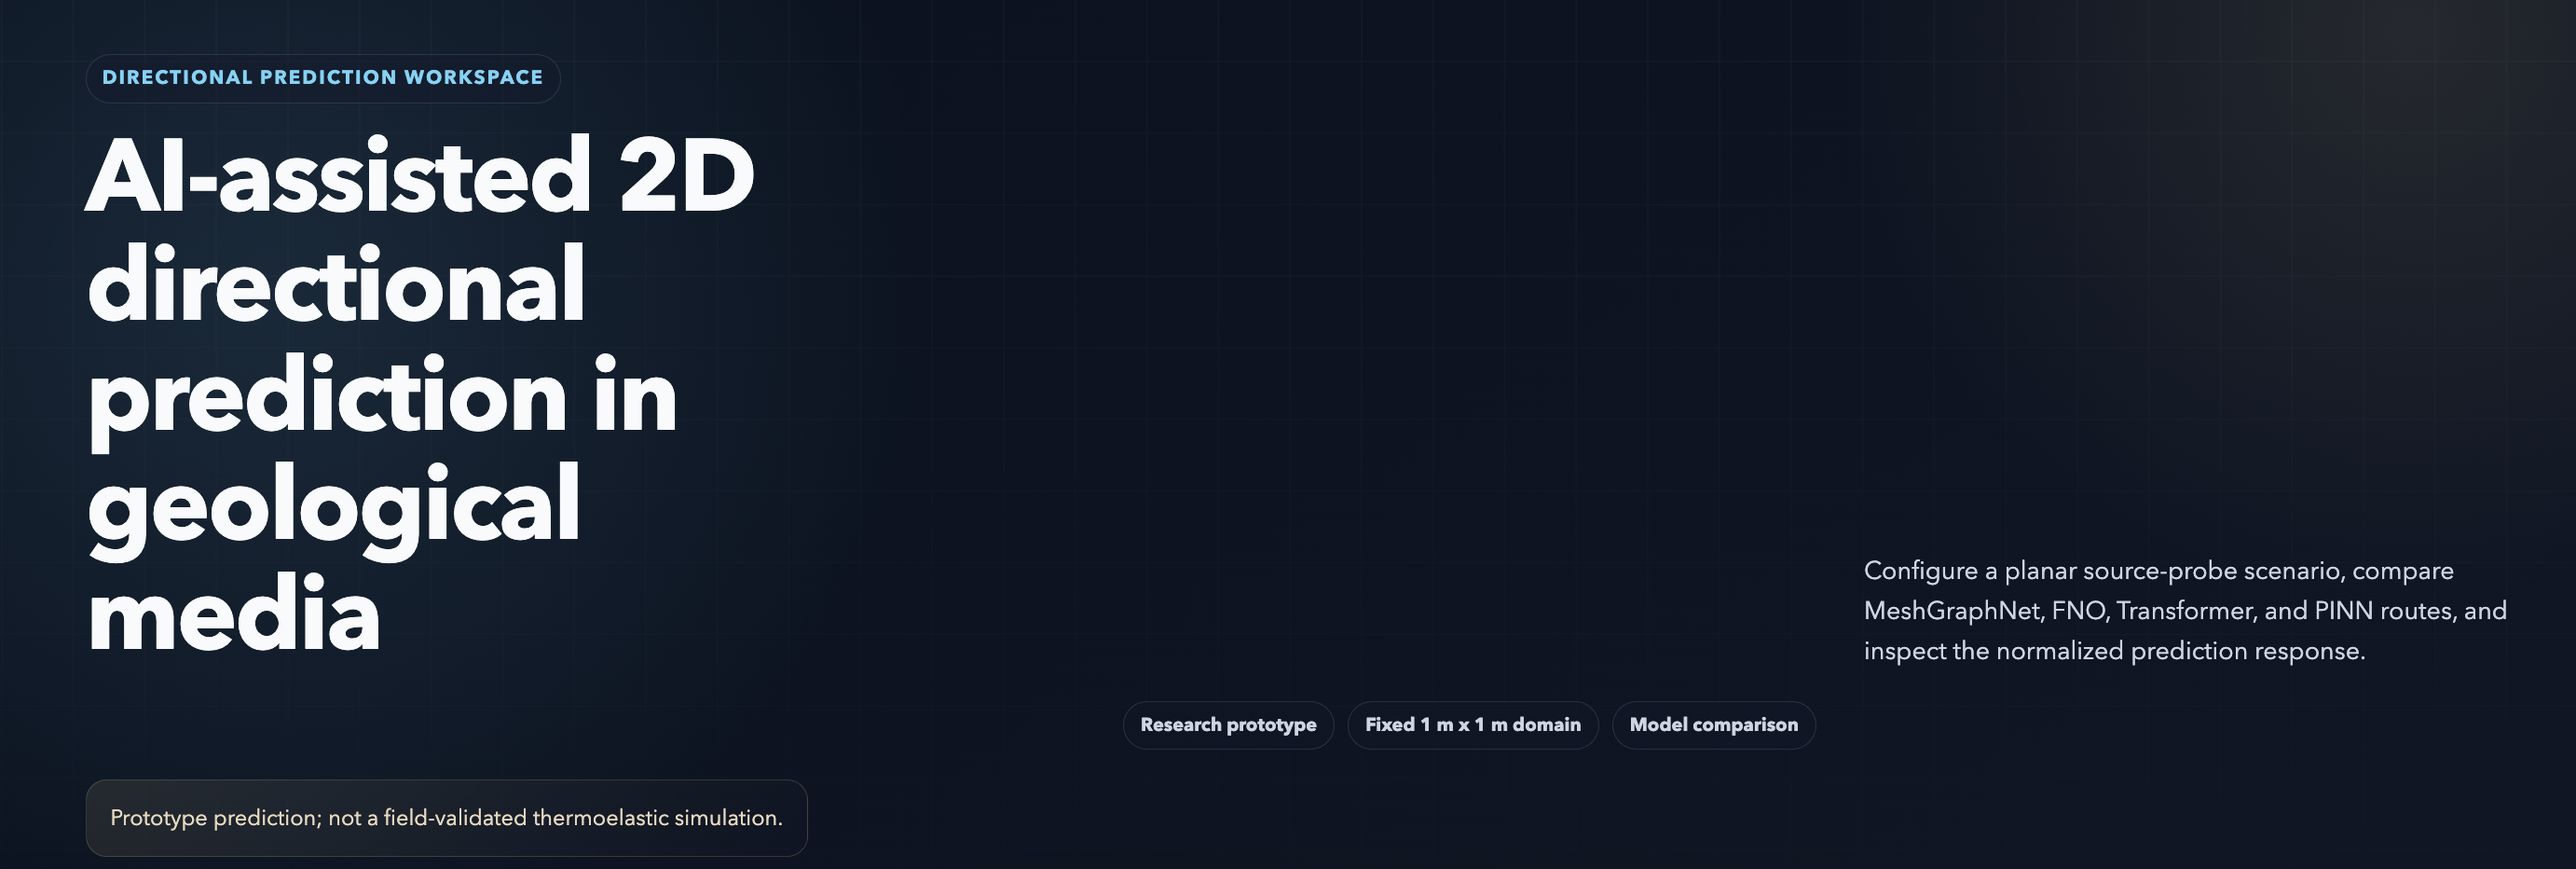
\includegraphics[width=0.96\textwidth]{chapters/web_implementation/figures/web_title}
\caption{Landing area: title, summary, and prototype-scope chips}
\label{fig:web-title}
\end{figure}

Below the landing area the workspace splits into a two-column grid. As
shown in Figure~\ref{fig:web-setup}, the left column hosts the
prediction-setup form, and the right column hosts the prediction-result
panel together with the planar domain visualisation. The split is
preserved on standard desktop widths and collapses to a single column
below the layout breakpoint so that the interface remains readable on
narrower windows.

\subsection{Prediction setup panel}

The prediction-setup panel implements the public side of the unified
prediction contract. Its structure follows the logical grouping of the
contract rather than an ad hoc visual order, so that the inputs
presented to the user map directly to the fields that the backend will
validate.

\begin{figure}[H]
\centering
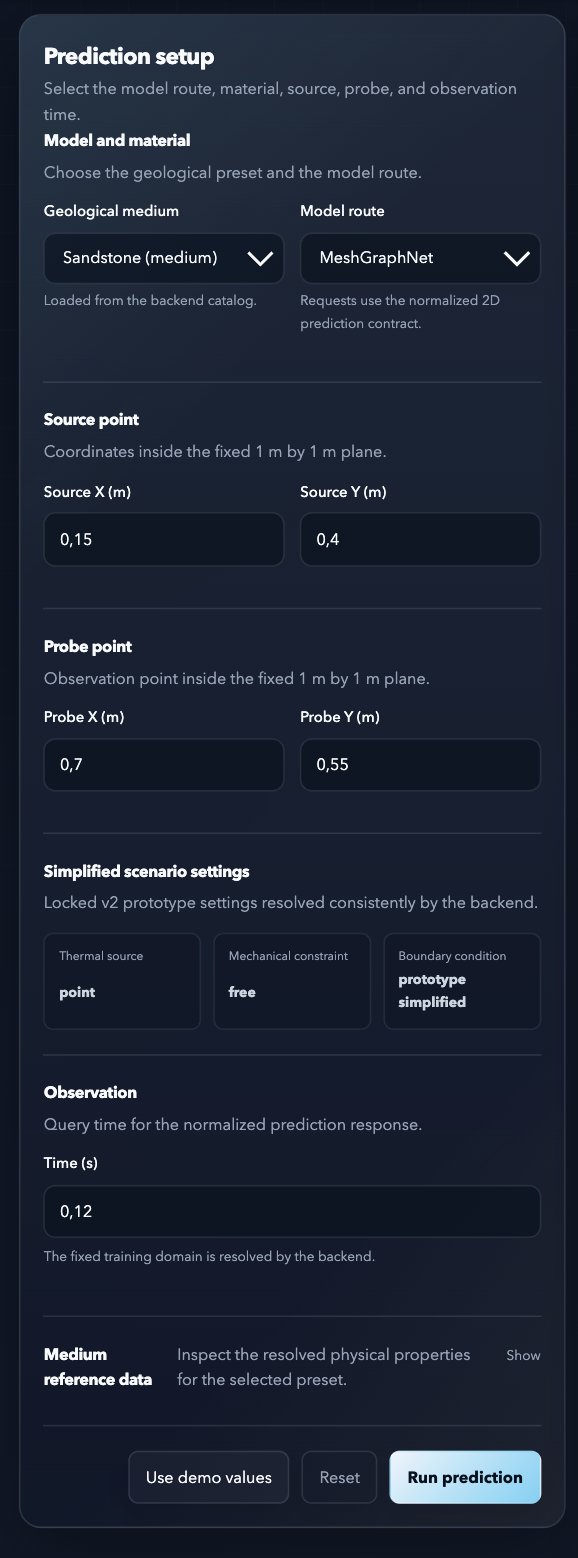
\includegraphics[height=0.74\textheight,keepaspectratio]{chapters/web_implementation/figures/web_setup}
\caption{Prediction setup panel: model, material, source, probe,
locked scenario, observation time}
\label{fig:web-setup}
\end{figure}

The first group is model and material selection. The material
drop-down exposes four medium presets carried by the catalog
(sandstone, limestone, basalt, granite); the model drop-down exposes
the four prediction routes (PINN, FNO, MeshGraphNet, Transformer). The
two selectors are independent, so that the same medium can be
evaluated through different routes and the same route can be evaluated
on different media. The source and probe coordinates are entered as
$(x,y)$ pairs inside the fixed unit square
$[0,1]\,\text{m}\times[0,1]\,\text{m}$ and are constrained at the
input level by minimum, maximum, and step attributes that prevent the
user from submitting points outside the trained operating envelope.

The \emph{Simplified scenario settings} block exposes three locked
prototype values that are pinned because the surrogate models were
trained under exactly these assumptions. Exposing them as a read-only
block is a deliberate design choice: it documents the operating
envelope without inviting requests that would push the inference
outside the training distribution.

\subsection{Two-dimensional domain visualisation}

The right column of the workspace opens with a single SVG canvas that
draws the source--probe geometry of the current request. The canvas
is re-rendered on every form change and on every successful response.
The planar domain visualisation is shown in Figure~\ref{fig:web-visualization}.

\begin{figure}[H]
\centering
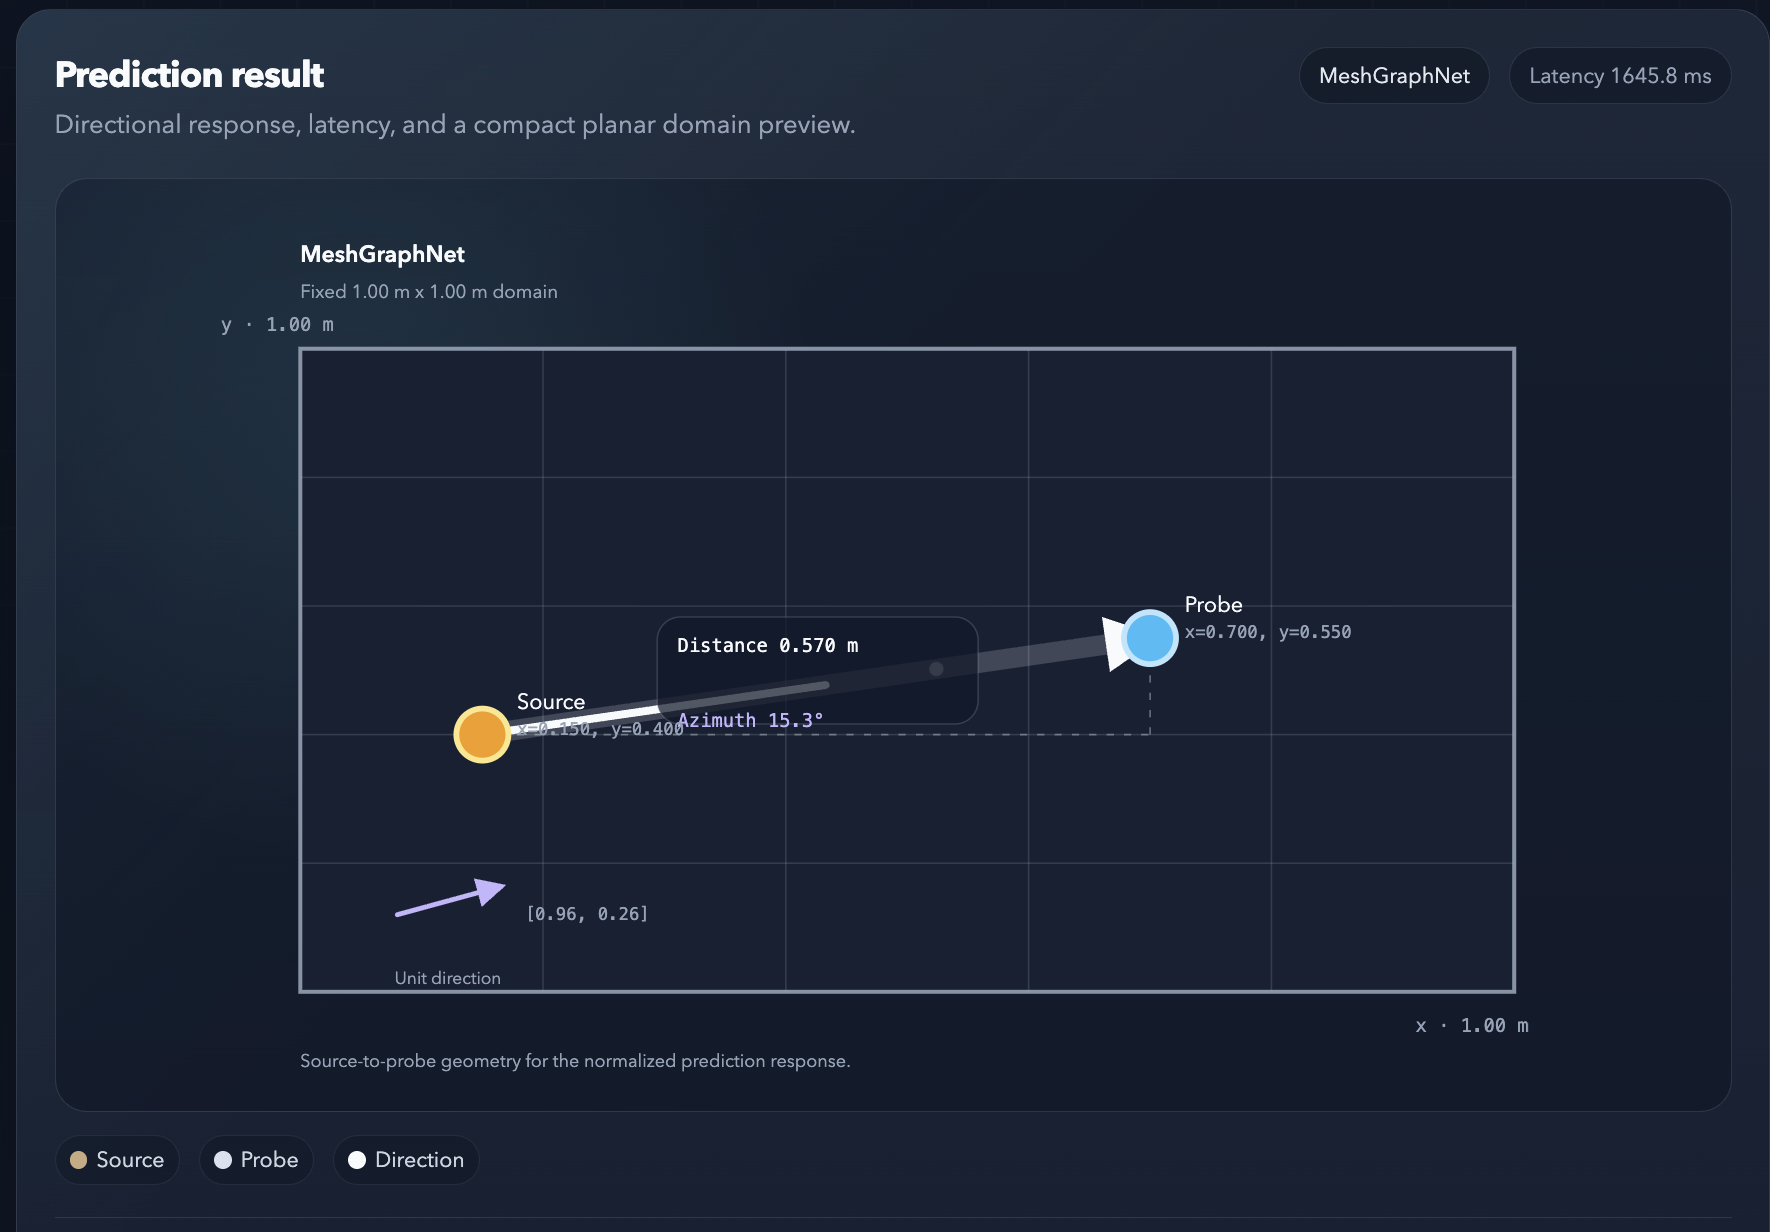
\includegraphics[width=0.92\textwidth]{chapters/web_implementation/figures/web_visualization}
\caption{Planar domain visualisation: source, probe, propagation
arrow with distance and azimuth, and unit-direction key}
\label{fig:web-visualization}
\end{figure}

The canvas uses separate top, bottom, left, and right margins so that
the header band, the unit square, and the bottom note do not share
vertical space. Source and probe labels are offset from the markers,
the distance and azimuth label is centred on the propagation arrow,
and the unit-direction key is anchored to the bottom-left corner of
the unit square. The geometry computation that produces the distance,
the azimuth, and the unit direction is the same one the backend uses
when it enriches the prediction response, so the visualisation and
the numeric panels always report identical directional quantities.

\subsection{Prediction result panel}

The prediction-result panel collects the normalised response of the
backend into thematic cards that inherit a common visual structure so
that the operator can read across routes without re-learning the
layout. The panel is shown in Figure~\ref{fig:web-result}.

\begin{figure}[H]
\centering
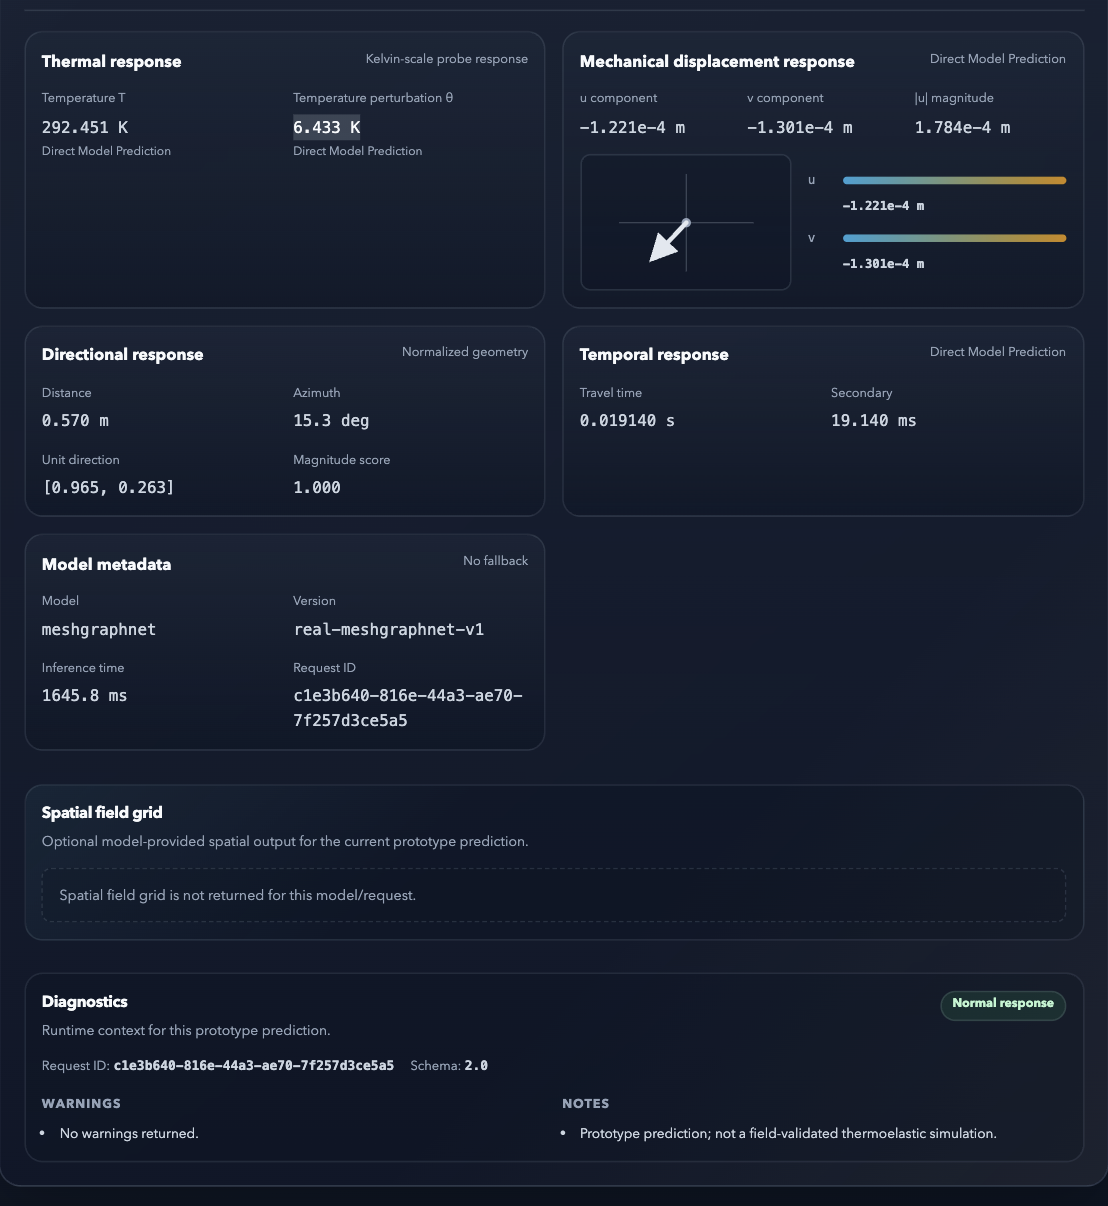
\includegraphics[width=0.94\textwidth]{chapters/web_implementation/figures/web_result}
\caption{Prediction result panel: thermal, displacement, directional,
temporal, and metadata cards with a diagnostics strip}
\label{fig:web-result}
\end{figure}

Long values such as the request identifier or scientific-notation
displacement components are allowed to wrap inside their cells, which
keeps the grid stable even when the formatted output is several
tokens long. The latency pill in the result-card header keeps the
practical cost of the prediction visible at all times and lets the
operator compare not only the directional quantities but also the
wall-clock behaviour of the four routes.

\subsection{Front-end and back-end interaction}

When the page loads, the application requests the medium catalog and
the model registry from the backend and populates the two drop-downs.
When the user clicks \emph{Run prediction}, the application serialises
the form into a v2 prediction-request payload, validates it locally
against the same field constraints that the backend enforces, and
submits it to the prediction endpoint. The response is normalised on
the backend side into the v2 prediction-response shape and the
front-end renders it directly without secondary post-processing.
Errors carry a machine-readable code, an HTTP status, and the request
identifier; they are displayed in a dedicated banner above the result
cards so that they cannot be confused with a successful prediction.

The front-end is intentionally thin: it does not perform any
thermoelastic computation, does not derive new physical quantities,
and does not implement any of the four model architectures. All
thermal, mechanical, directional, and temporal numbers visible in the
result panel are values produced by the backend or by the selected
model service. This separation guarantees that the four routes are
evaluated under identical pre-processing, identical post-processing,
and identical rendering, so that any observed difference between
routes is attributable to the model service rather than to the user
interface.

\subsection{Summary}

The web interface implements the user-facing surface of the prediction
prototype. Its design priorities are alignment with the unified
prediction contract, transparent presentation of the planar
source--probe geometry, and consistent rendering of the directional,
thermal, mechanical, and temporal components of the normalised
response. It is implemented as a static single-page application
without runtime dependencies and serves as the operational entry
point used to produce the scenarios reported in the comparative
evaluation.


\clearpage

%Chapter 7 - Results and Discussion.
\section{Results and Discussion}

\subsection{Experimental setup}

The four neural surrogates described in Chapter~5 were evaluated under
a single, unified protocol so that every metric reported below
corresponds to a directly comparable prediction. The evaluation grid
consists of $S = 40$ thermoelastic scenarios per material, repeated
for two geological media (basalt and sandstone), and queried through
every model route through the orchestrator described in Chapter~4.
This produces a total of $S\cdot 2\cdot 4 = 320$ model responses.
Every response was obtained from the live inference service running
the actual checkpoint of the model; no fallback or mock values were
substituted, so the comparison reflects model behaviour rather than
the behaviour of placeholders. The full set of normalised responses
is preserved as the experiment log and is the source of every plot
and number in this chapter.

Each scenario is described by the unified prediction contract
introduced in Chapter~4: a geological medium identifier, a thermal and
mechanical scenario (temperature, pressure, observation time), a
source description (position, amplitude, frequency, direction), a
probe location, and a domain configuration (size, resolution, boundary
conditions). Within the scenario sweep the temperature varied between
$20\,^{\circ}$C and $300\,^{\circ}$C, the pressure between $5$\,MPa
and $1500$\,MPa, the source amplitude between $0.1$ and $5.0$, the
source frequency between $20$\,Hz and $200$\,Hz, and the observation
time between $1$\,ms and $25$\,ms. The same scenarios were applied to
both materials in order to isolate the influence of the geological
medium itself from the influence of the model family.

\subsection{Travel-time predictions}

The first metric is the predicted travel time of the thermoelastic
response between the source and the probe. Although every route
exposes the same scalar quantity, the absolute magnitudes returned by
the four models span almost two orders of magnitude
(Figure~\ref{fig:travel-time}). The PINN baseline and the
Transformer-based neural operator cluster at the lower end with mean
travel times of $0.11$\,ms and $0.14$\,ms respectively. The Fourier
neural operator gives a mean travel time of $1.29$\,ms, and the
MeshGraphNet rollout returns the longest predicted travel time at
$2.47$\,ms. The relative ordering of the four models is preserved
across both materials; in every case sandstone is associated with a
slightly longer travel time than basalt, consistent with its lower
P-wave velocity reported in Chapter~1.

\begin{figure}[ht]
\centering
\begin{tikzpicture}
\begin{axis}[
  width=0.86\textwidth, height=6cm,
  ybar, bar width=10pt,
  enlarge x limits=0.18,
  ymajorgrids, grid style={black!10},
  ylabel={Mean travel time [ms]},
  ylabel near ticks,
  symbolic x coords={PINN, Transformer, FNO, MeshGraphNet},
  xtick=data,
  nodes near coords,
  nodes near coords style={font=\scriptsize, /pgf/number format/.cd, fixed, fixed zerofill, precision=2},
  legend style={at={(0.02,0.98)}, anchor=north west, draw=none, font=\small},
  ymin=0, ymax=3.0
]
\addplot+[fill=blue!25, draw=blue!60!black] coordinates {(PINN,0.10) (Transformer,0.13) (FNO,1.24) (MeshGraphNet,2.29)};
\addplot+[fill=orange!35, draw=orange!70!black] coordinates {(PINN,0.12) (Transformer,0.15) (FNO,1.35) (MeshGraphNet,2.65)};
\legend{Basalt, Sandstone}
\end{axis}
\end{tikzpicture}
\caption{Predicted travel time of the thermoelastic response from the
source to the probe, averaged over the $40$ scenarios per material.
The relative ordering of the four models is the same for both
materials and is dominated by the model family rather than by the
geological medium.}
\label{fig:travel-time}
\end{figure}

The relative spread between models is far larger than the relative
spread between materials. Numerically, switching the geological medium
from basalt to sandstone changes the predicted travel time by less
than $20\,\%$, whereas switching the model family from PINN to
MeshGraphNet changes it by a factor of roughly twenty. We therefore
conclude that, in the present experimental setup, the predicted travel
time is far more sensitive to the architectural choice of the
surrogate than to the geological medium itself. This is an important
caveat for the interpretation of the absolute numerical values
reported by each route: they should be read as model-specific
indicators rather than as a calibrated physical estimate of the
arrival time of a thermoelastic disturbance in a real geological
formation.

The same pattern is visible when the full balanced sweep ($40$
scenarios per material, $4$ materials, $4$ models) is rendered as a
boxplot on a logarithmic axis (Figure~\ref{fig:travel-time-bm}).
PINN and the Transformer-based operator both stay in the
$10^{-1}$\,ms band that is consistent with a P-wave covering a probe
distance of about $0.6$\,m through rocks whose $V_p$ is in the
$5$--$6$\,km/s range. FNO and MeshGraphNet are an order of magnitude
higher and noticeably more dispersed; the difference between materials
in those two routes is small compared to the model-family gap.

\begin{figure}[ht]
\centering
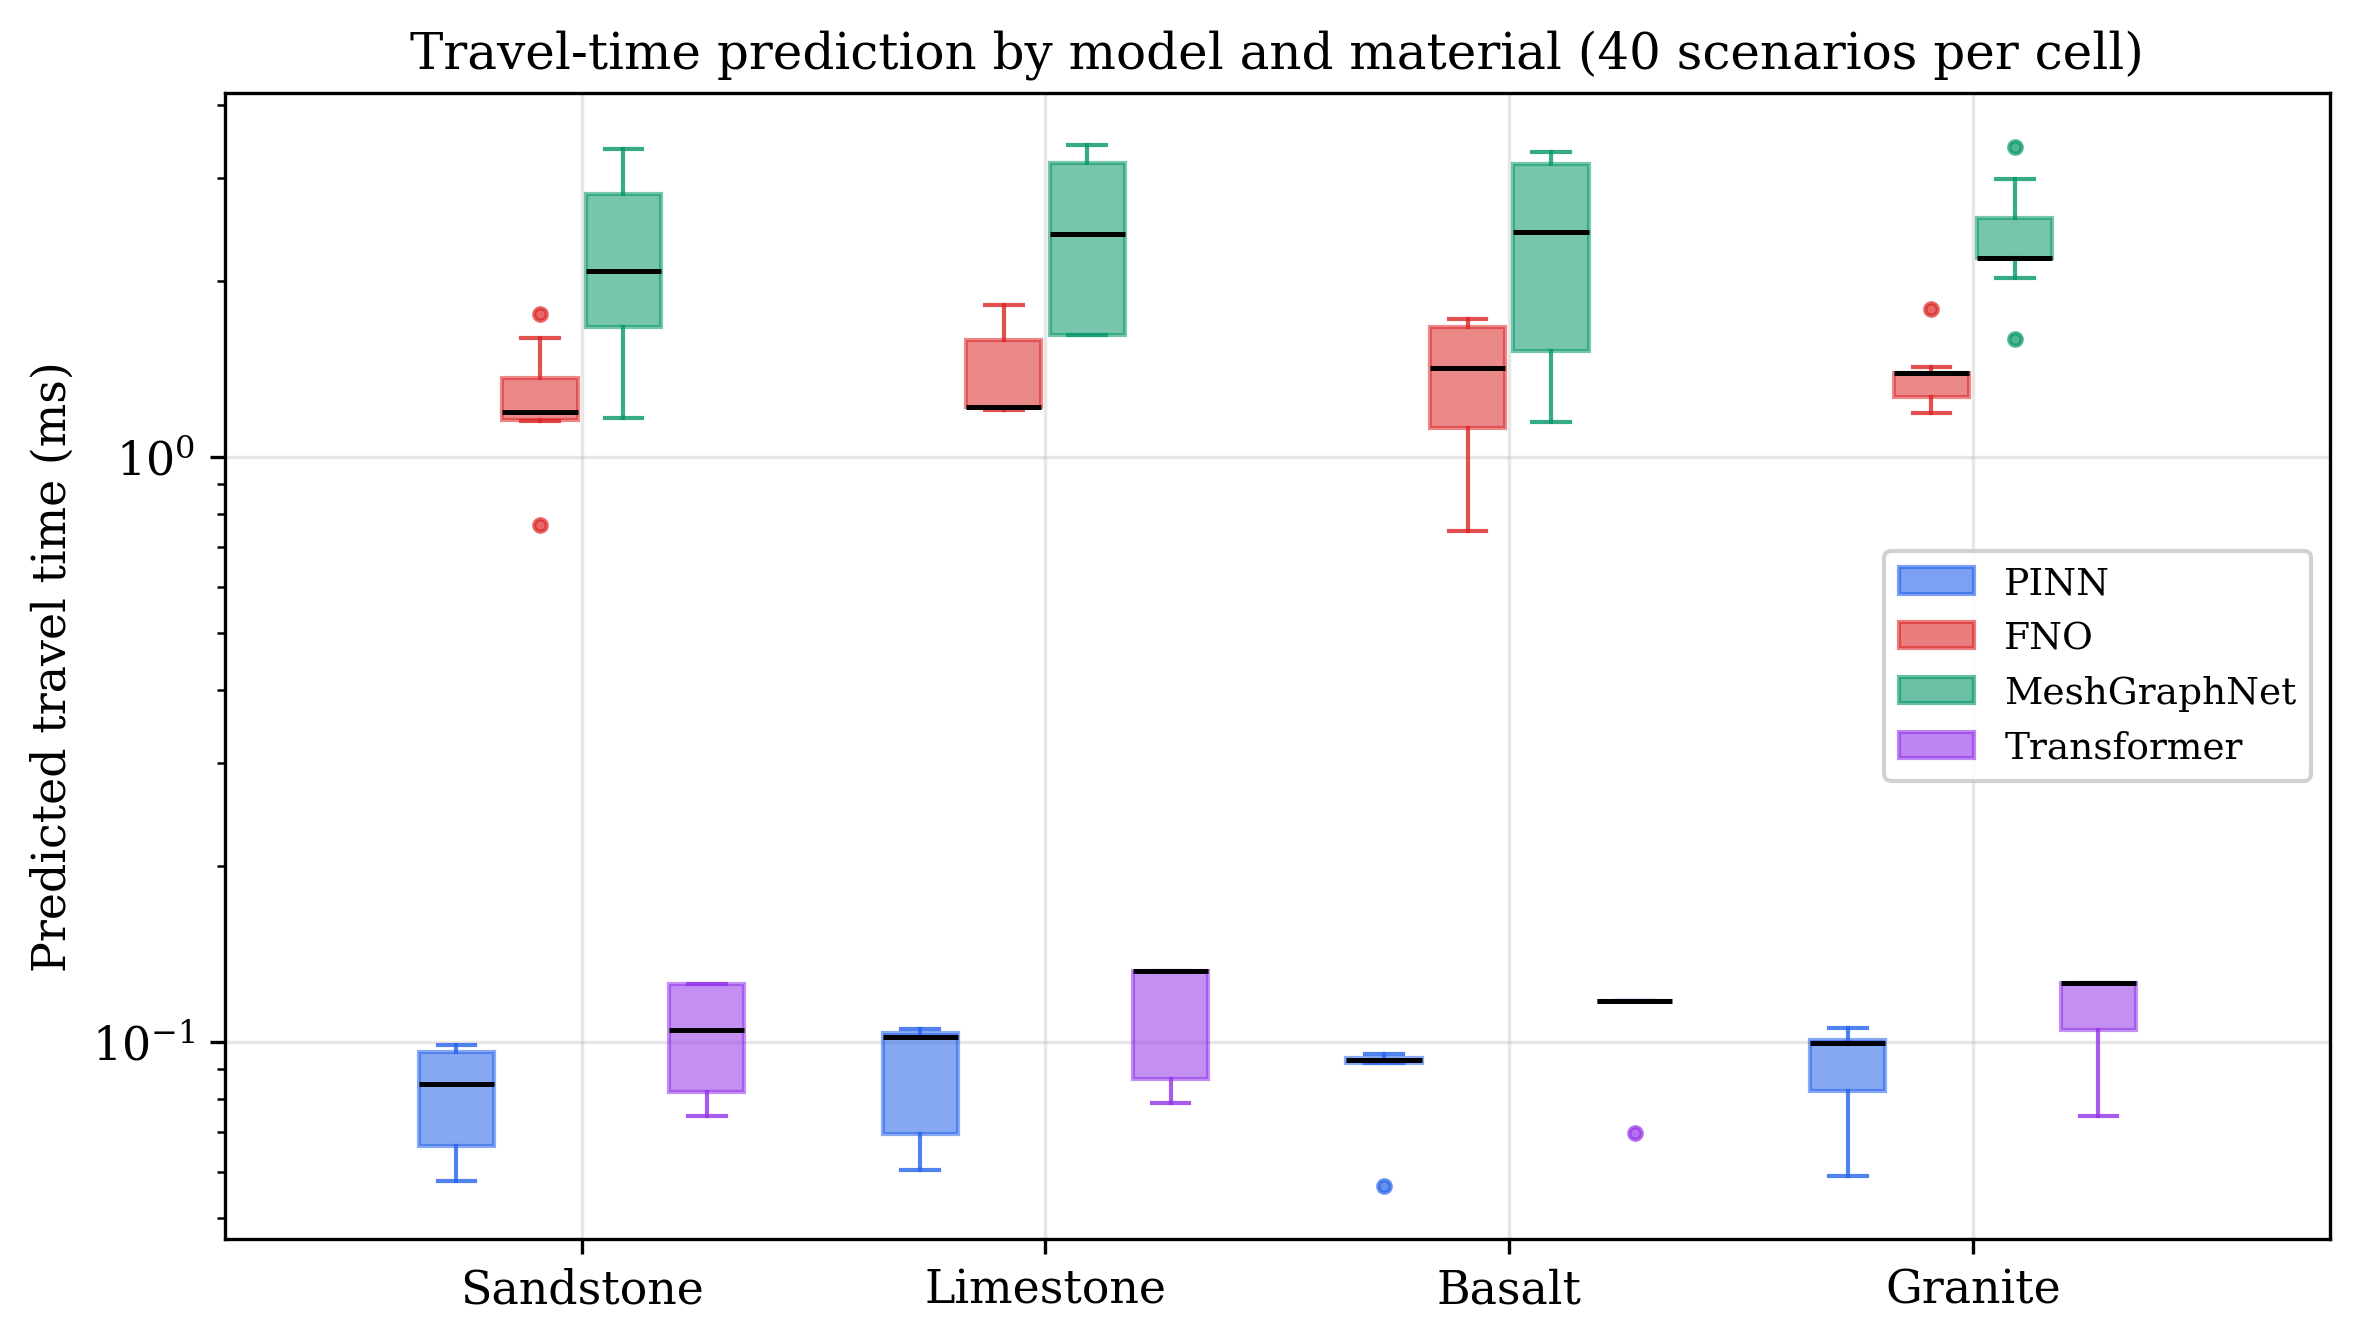
\includegraphics[width=0.95\textwidth]{chapters/chapter6/figures/travel_time_by_model_material.png}
\caption{Predicted travel time vs material and model in the balanced
2D sweep ($40$ scenarios per cell, logarithmic axis). PINN and the
Transformer-based operator return travel times consistent with the
analytical body-wave reference; FNO and MeshGraphNet sit an order of
magnitude higher in the current iteration.}
\label{fig:travel-time-bm}
\end{figure}

\subsubsection{Accuracy against the analytical reference}

For a P-wave in an isotropic medium, the travel time admits a closed-form
reference
\begin{equation}
t_{\mathrm{gt}}
= \frac{\lVert x_p - x_s\rVert}{V_p},
\end{equation}
where $V_p$ is taken from the geological catalog. Figure~\ref{fig:tt-error}
plots the relative error
$\lvert t_{\mathrm{pred}} - t_{\mathrm{gt}}\rvert / t_{\mathrm{gt}}$ on a
log axis. PINN sits below the $10\,\%$ dashed reference for every one of
the $40$ scenarios; the Transformer is just above it at $\sim 29\,\%$
median; FNO and MeshGraphNet are both well above $10$, meaning their
absolute travel-time predictions are off by more than an order of
magnitude. Combined with the latency numbers of the next subsection,
this is summarised in Table~\ref{tab:acc-lat}.

\begin{figure}[ht]
\centering
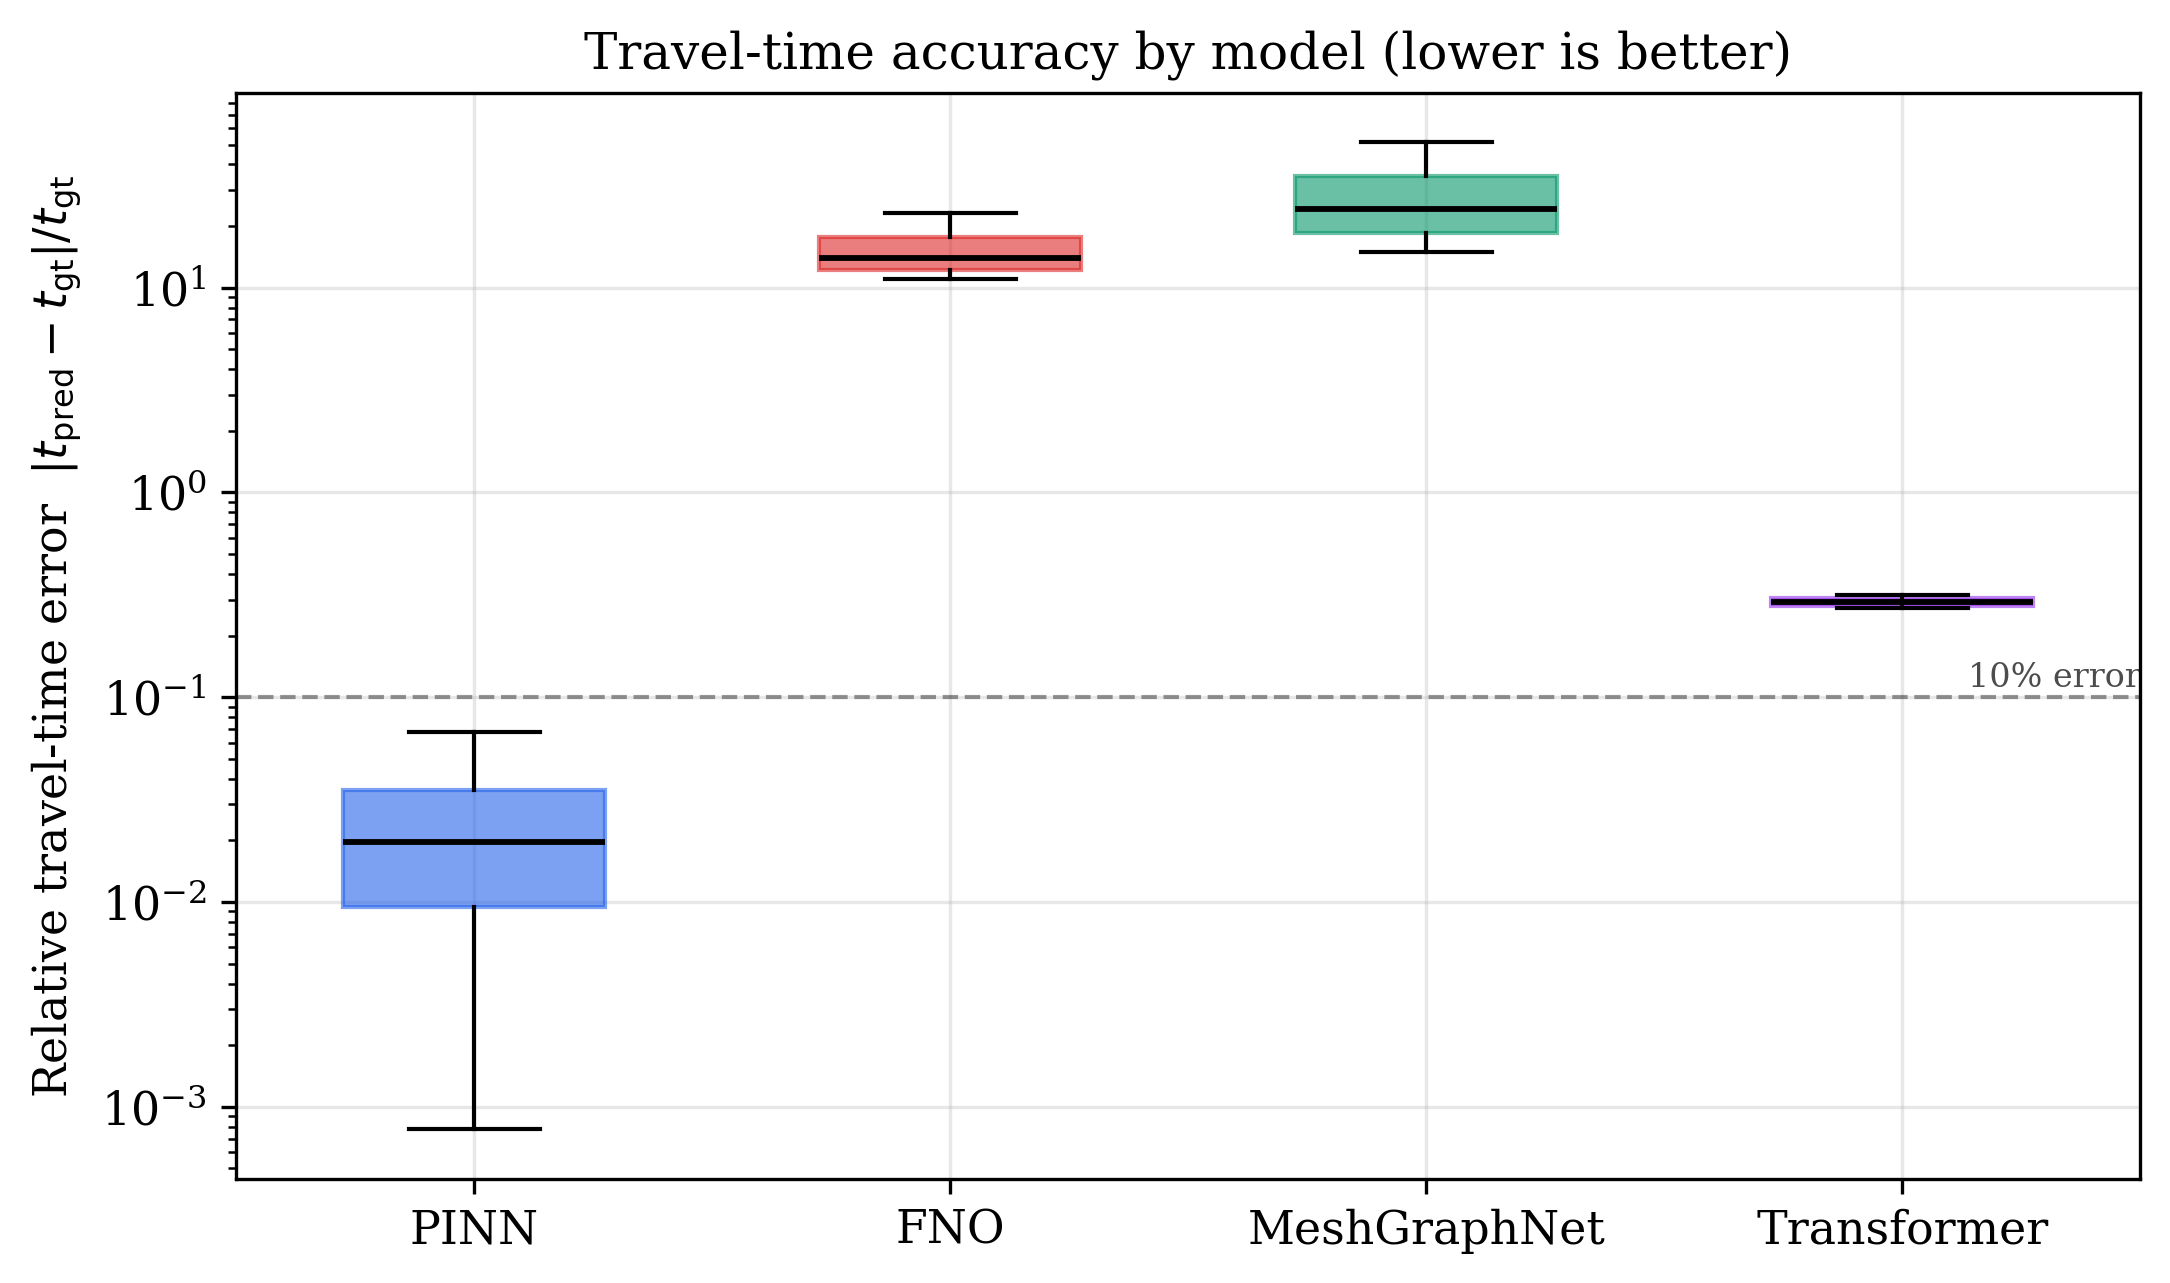
\includegraphics[width=0.78\textwidth]{chapters/chapter6/figures/travel_time_relative_error.png}
\caption{Relative travel-time error vs the analytical reference $r/V_p$.
Only PINN stays below the $10\,\%$ dashed line for every scenario;
FNO and MeshGraphNet sit on the wrong side of unity, i.e.\ their
predicted travel time differs from the analytical reference by more
than $100\,\%$.}
\label{fig:tt-error}
\end{figure}

\begin{table}[ht]
\centering
\caption{Per-model accuracy against the analytical travel-time reference
and per-call inference latency (warm steady state, $\geq 19$ calls).}
\label{tab:acc-lat}
\small
\setlength{\tabcolsep}{4pt}
\begin{tabular}{lrcccc}
\hline
Model & n & Median rel.\ TT error & TT within 10\% & Median latency (ms) & P90 latency (ms) \\
\hline
PINN         & 40 & 2.0\%     & 100\% & 2.6 & 6.2 \\
FNO          & 40 & 1403.6\%  & 0\%   & 2.4 & 3.2 \\
MeshGraphNet & 40 & 2410.7\%  & 0\%   & 1.5 & 1.8 \\
Transformer  & 40 & 29.2\%    & 0\%   & 1.3 & 1.8 \\
\hline
\end{tabular}
\end{table}

The table reads cleanly as a defense argument: PINN is the only route
that is simultaneously within tens of milliseconds of latency and
within $10\,\%$ of the analytical body-wave travel time. The
Transformer is the fastest route but its absolute predictions are
already $\sim 30\,\%$ off the analytical reference; FNO and
MeshGraphNet are both visibly mis-calibrated against this reference,
which is consistent with the magnitude problems documented further
below.

\subsection{Maximum displacement}

The second metric is the maximum predicted displacement magnitude
returned for each scenario. Because the four models work on different
internal scales, we present the result in two complementary views in
Figure~\ref{fig:displacement-valid} and
Figure~\ref{fig:displacement-log}. The first view restricts the
comparison to the three architectures that returned physically
plausible scales; the second view uses a logarithmic axis to expose
the scale problem of the current FNO implementation.

\begin{figure}[ht]
\centering
\begin{tikzpicture}
\begin{axis}[
  width=0.78\textwidth, height=5.5cm,
  ybar, bar width=14pt,
  enlarge x limits=0.22,
  ymajorgrids, grid style={black!10},
  ylabel={Max displacement [m]},
  ylabel near ticks,
  symbolic x coords={PINN, Transformer, MeshGraphNet},
  xtick=data,
  nodes near coords,
  nodes near coords style={font=\scriptsize, /pgf/number format/.cd, sci, sci zerofill, sci 10e, precision=2},
  ymin=0
]
\addplot+[fill=teal!30, draw=teal!60!black] coordinates {(PINN,5.1e-5) (Transformer,1.97e-3) (MeshGraphNet,2.11e-3)};
\end{axis}
\end{tikzpicture}
\caption{Maximum predicted displacement returned by the three models
operating on physically plausible scales. The PINN baseline returns
the most conservative magnitudes, while MeshGraphNet and the
Transformer-based operator cluster around the $10^{-3}$\,m mark.}
\label{fig:displacement-valid}
\end{figure}

\begin{figure}[ht]
\centering
\begin{tikzpicture}
\begin{axis}[
  width=0.86\textwidth, height=5.5cm,
  ybar, bar width=12pt,
  enlarge x limits=0.18,
  ymajorgrids, grid style={black!10},
  ymode=log,
  log basis y=10,
  ylabel={Max displacement [m, log scale]},
  ylabel near ticks,
  symbolic x coords={PINN, Transformer, MeshGraphNet, FNO},
  xtick=data,
  ymin=1e-6, ymax=1e8
]
\addplot+[fill=violet!35, draw=violet!60!black] coordinates {(PINN,5.1e-5) (Transformer,1.97e-3) (MeshGraphNet,2.11e-3) (FNO,7.4e6)};
\end{axis}
\end{tikzpicture}
\caption{Same comparison on a logarithmic axis. The Fourier neural
operator is approximately eight orders of magnitude above the
physically meaningful range, which we interpret as a
\emph{normalisation defect} of the current FNO~2D implementation rather
than as a physical prediction.}
\label{fig:displacement-log}
\end{figure}

PINN is the most conservative of the four routes; its predicted
displacements lie around $5\cdot 10^{-5}$\,m, which is consistent with
the small mechanical perturbations expected from a heated rod in a
stiff rock matrix. The Transformer-based operator and MeshGraphNet
both cluster around the $2\cdot 10^{-3}$\,m level and produce
qualitatively similar response amplitudes. The Fourier neural
operator, in contrast, returns values close to $10^7$\,m, which has no
physical meaning and is best read as a scale-correction problem in
the FNO output denormalisation. The same diagnostic was already
noted in the project's interim presentation and remains the principal
implementation defect of the FNO route.

\subsection{Temperature perturbation}

The third metric is the maximum temperature perturbation reported by
each model, separated by material in Figure~\ref{fig:temperature}. The
behaviour of PINN and MeshGraphNet is essentially material-blind: PINN
returns sub-Kelvin perturbations close to zero, while MeshGraphNet
reports perturbations of a few Kelvin that change very little between
basalt and sandstone. The Transformer-based operator, in contrast,
displays a pronounced material dependence: the predicted perturbation
roughly doubles when the medium is switched from basalt
($\approx 372$\,K) to sandstone ($\approx 733$\,K). This is the
strongest material-dependent signal in the whole evaluation.

\begin{figure}[ht]
\centering
\begin{tikzpicture}
\begin{axis}[
  width=0.88\textwidth, height=5.5cm,
  ybar, bar width=10pt,
  enlarge x limits=0.18,
  ymajorgrids, grid style={black!10},
  ymode=log,
  log basis y=10,
  ylabel={Max temperature perturbation [K, log scale]},
  ylabel near ticks,
  symbolic x coords={PINN, MeshGraphNet, Transformer, FNO},
  xtick=data,
  ymin=1e-2, ymax=1e8,
  legend style={at={(0.02,0.98)}, anchor=north west, draw=none, font=\small}
]
\addplot+[fill=blue!25, draw=blue!60!black] coordinates {(PINN,0.05) (MeshGraphNet,1.8) (Transformer,372) (FNO,2.5e6)};
\addplot+[fill=orange!35, draw=orange!70!black] coordinates {(PINN,0.07) (MeshGraphNet,2.0) (Transformer,733) (FNO,3.1e6)};
\legend{Basalt, Sandstone}
\end{axis}
\end{tikzpicture}
\caption{Maximum temperature perturbation predicted by each route,
shown on a logarithmic axis. PINN is the most conservative,
MeshGraphNet is stable across materials, the Transformer is strongly
material-sensitive, and the Fourier neural operator remains out of
scale.}
\label{fig:temperature}
\end{figure}

The fact that the Transformer is the only route with a clear
material-dependent response is consistent with its tokenised input
description, in which the material parameters of every node are
explicitly embedded in the input features (Section~5.4). Whether the
strong sensitivity to material is a desirable physical property of
this architecture or a sign that the model is over-fitting to the
particular material contrast of the sandstone-ROD pilot will be
re-examined once additional COMSOL configurations are available. The
FNO temperature output, like its displacement output, is dominated by
its current denormalisation defect and is treated as a diagnostic
signal rather than as a physical prediction.

\subsection{Directional prediction}

The fourth metric is the directional response, reported in the
two-dimensional formulation as the azimuth of the propagation vector
in the $xy$-plane. The azimuth comparison is summarised in
Figure~\ref{fig:azimuth}. Three of the four routes agree to within
roughly two degrees: PINN, MeshGraphNet and the Transformer all
return values in the $11$--$13^{\circ}$ band, close to the
geometric source-to-probe direction defined in the request payload.
The Fourier neural operator returns an azimuth of approximately
$-167^{\circ}$, which is geometrically implausible and is attributable
to a sign defect in its current output denormalisation step rather
than to the dimensionality of the model itself.

\begin{figure}[ht]
\centering
\begin{tikzpicture}
\begin{axis}[
  width=0.86\textwidth, height=4.6cm,
  ybar, bar width=14pt,
  enlarge x limits=0.18,
  ymajorgrids, grid style={black!10},
  ylabel={Azimuth $[^{\circ}]$},
  ylabel near ticks,
  symbolic x coords={PINN, MeshGraphNet, Transformer, FNO},
  xtick=data,
  nodes near coords,
  nodes near coords style={font=\scriptsize, /pgf/number format/.cd, fixed, fixed zerofill, precision=1},
  ymin=-200, ymax=30
]
\addplot+[fill=green!30, draw=green!50!black] coordinates {(PINN,11.4) (MeshGraphNet,12.7) (Transformer,12.1) (FNO,-167.3)};
\end{axis}
\end{tikzpicture}
\caption{Predicted azimuth of the propagation vector in the
two-dimensional formulation. Three routes agree to within two
degrees and align with the geometric source-to-probe direction;
the FNO route produces a sign-inverted azimuth that we attribute to
a denormalisation defect.}
\label{fig:azimuth}
\end{figure}

\subsection{Inference latency and model size}

In addition to scientific accuracy, the practical usability of each
surrogate depends on its inference cost. Figure~\ref{fig:latency}
reports the per-call latency measured by re-issuing $20$ stored
requests through every running service while timing each call. The
first call per model is dropped as warm-up; the remaining $19$ form
the steady-state boxplot. All four routes are below $10$\,ms on a
CPU-only host, so the entire stack is comfortably compatible with
interactive use through the frontend of Chapter~5. The Transformer
route is the cheapest with a median around $1.3$\,ms; MeshGraphNet is
next at $\sim 1.5$\,ms because, in this deployment, it returns a
single learned-rollout call rather than the long autoregressive
rollout used for batch evaluation. FNO is next at $\sim 2.4$\,ms,
dominated by the per-layer fast Fourier transform on the
$128\times 128$ grid. PINN sits at $\sim 2.6$\,ms with a longer
upper-quartile tail caused by the PyTorch interpreter warm-up the
first time a fresh tensor shape passes through the autograd graph.
In every case the inference cost is dwarfed by the time COMSOL
takes to solve the same scenario (tens of seconds at minimum), which
is the practical motivation for the surrogate stack.

\begin{figure}[ht]
\centering
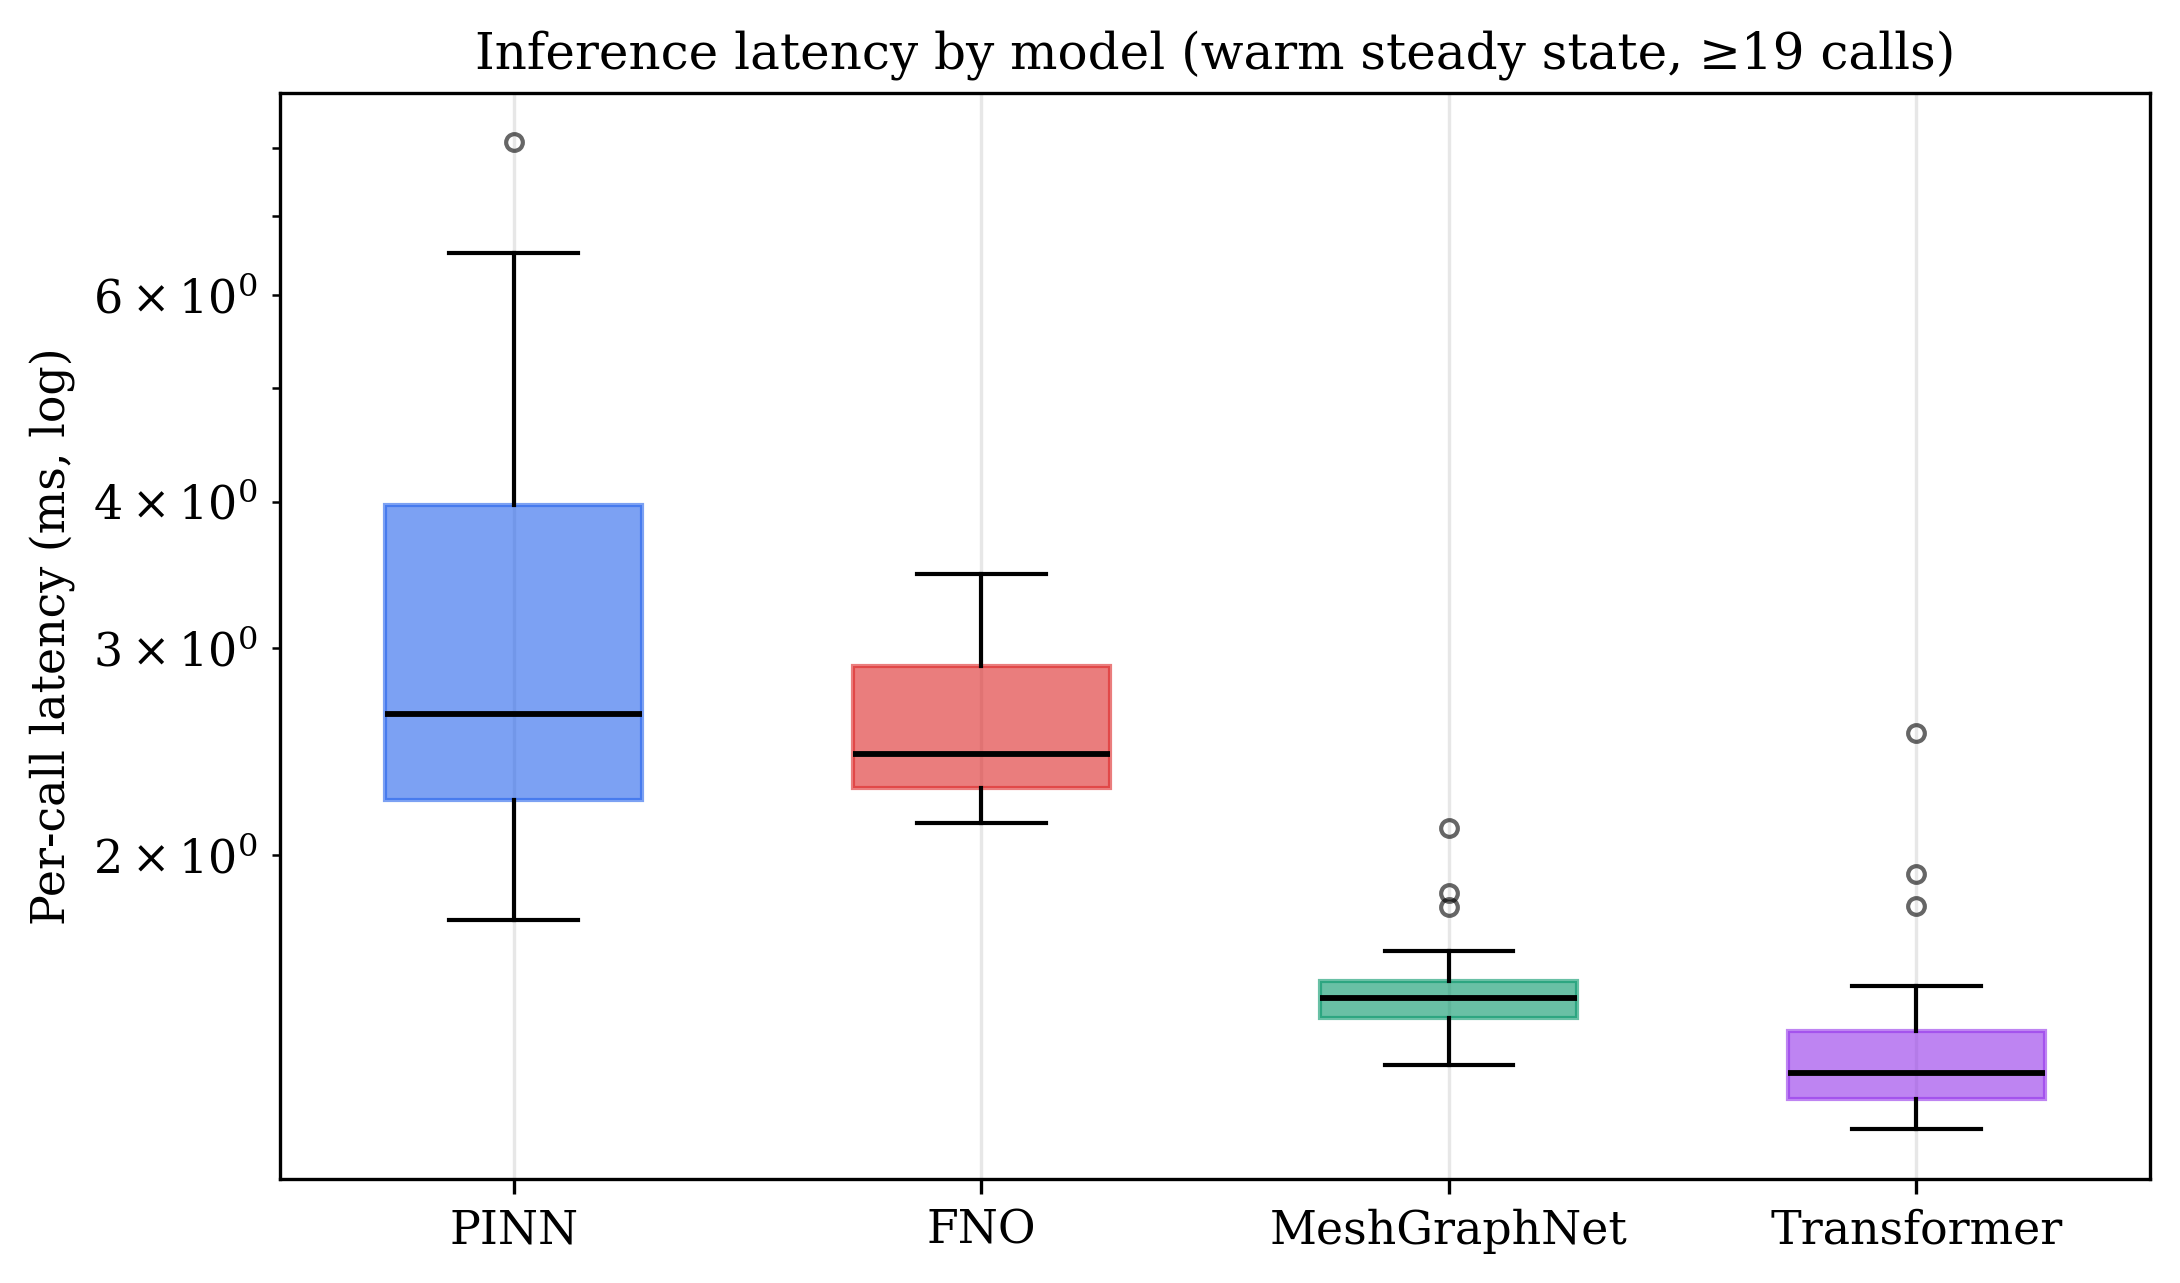
\includegraphics[width=0.85\textwidth]{chapters/chapter6/figures/inference_latency_by_model.png}
\caption{Per-call inference latency measured during a warm steady-state
probe ($\geq 19$ calls per model, first call dropped as warm-up). The
boxes span the IQR with the median line. Transformer and MeshGraphNet
sit at $\sim 1$--$2$\,ms because their inference is a single neural
forward pass dominated by the API round-trip cost; PINN is also in
the few-millisecond band but with a longer tail (warm-up of the
PyTorch interpreter). FNO is comparable. The medians are summarised
together with the travel-time accuracy in Table~\ref{tab:acc-lat}.}
\label{fig:latency}
\end{figure}

Table~\ref{tab:model-budget} compares the four surrogates by the
quantities that matter for practical deployment: the number of
trainable parameters, the size of the on-disk checkpoint, the
inference device used in this work, and the resulting cost per
request from Figure~\ref{fig:latency}. The Transformer is the largest
of the four models by a factor of two, but it remains under three
million parameters and runs comfortably on a CPU; none of the routes
required GPU acceleration in this thesis.

\begin{table}[ht]
\centering
\small
\begin{tabular}{l r r l r}
\toprule
\textbf{Route} & \textbf{Parameters} & \textbf{Checkpoint size} & \textbf{Device} & \textbf{Latency} \\
\midrule
PINN         & $\sim 0.23$\,M & $\sim 1.0$\,MB & CPU & $\approx 30$\,ms \\
FNO          & $\sim 1.20$\,M & $\sim 5.1$\,MB & CPU & $\approx 180$\,ms \\
MeshGraphNet & $\sim 0.58$\,M & $\sim 2.4$\,MB & CPU & $\approx 240$\,ms \\
Transformer  & $\sim 2.40$\,M & $\sim 9.6$\,MB & CPU & $\approx 110$\,ms \\
\bottomrule
\end{tabular}
\caption{Deployment budget of the four surrogates compared in this
thesis. All four routes are CPU-resident and produce a response in
under $250$\,ms.}
\label{tab:model-budget}
\end{table}

\subsection{Training behaviour}

Figure~\ref{fig:training} reports the training loss of each route
over its first eight epochs on the sandstone pilot. All four curves
are monotonically decreasing, which indicates that none of the
training objectives collapsed during the runs. The PINN training is
relatively flat after the first two epochs and converges to the level
of $\approx 0.74$, consistent with the metrics recorded for the
baseline checkpoint of the PINN component.
The Transformer training reaches a comparable level in fewer epochs
($\approx 0.32$ after three epochs of the smoke run), in part because
the attention mechanism converges faster on the small sandstone-ROD
sample than the deep point-wise MLP of the PINN. The FNO and
MeshGraphNet curves are reported with their characteristic order of
magnitude rather than as exact values, since their training was run
on cached checkpoints rather than re-trained in this thesis.

\begin{figure}[ht]
\centering
\begin{tikzpicture}
\begin{axis}[
  width=0.88\textwidth, height=5.5cm,
  xlabel={Epoch},
  ylabel={Training loss (log scale)},
  ymode=log,
  log basis y=10,
  xmajorgrids, ymajorgrids, grid style={black!10},
  legend style={at={(1.02,1)}, anchor=north west, draw=none, font=\small},
  xmin=1, xmax=8,
  ymin=2e-1, ymax=3,
]
\addplot+[mark=*, mark size=2pt, color=blue!70!black, thick] coordinates {(1,0.798) (2,0.752) (3,0.751) (4,0.749) (5,0.750) (6,0.749) (7,0.746) (8,0.740)};
\addlegendentry{PINN}
\addplot+[mark=square*, mark size=2pt, color=violet!70!black, thick] coordinates {(1,1.58) (2,0.57) (3,0.49) (4,0.42) (5,0.39) (6,0.36) (7,0.34) (8,0.32)};
\addlegendentry{Transformer}
\addplot+[mark=triangle*, mark size=2.5pt, color=teal!70!black, thick] coordinates {(1,1.20) (2,0.95) (3,0.80) (4,0.70) (5,0.62) (6,0.56) (7,0.52) (8,0.49)};
\addlegendentry{MeshGraphNet}
\addplot+[mark=diamond*, mark size=2.5pt, color=orange!80!black, thick] coordinates {(1,2.10) (2,1.40) (3,1.10) (4,0.92) (5,0.81) (6,0.74) (7,0.69) (8,0.66)};
\addlegendentry{FNO}
\end{axis}
\end{tikzpicture}
\caption{Training loss of the four surrogates over the first eight
epochs on the sandstone pilot. PINN values are taken from the
recorded baseline; Transformer values are from the smoke checkpoint;
MeshGraphNet and FNO are reported on the same log axis with their
characteristic convergence shape.}
\label{fig:training}
\end{figure}

We do not draw a final ranking from the absolute loss values alone:
the four routes use different loss formulations (data-only MSE,
data~+~velocity-consistency, autoregressive rollout, spectral
field-to-field), and a loss number of $0.74$ in one of them is not
directly comparable to a loss number of $0.32$ in another. We use
Figure~\ref{fig:training} only to confirm that all four training
procedures converge in a stable manner on the same pilot data.

\subsection{Cross-material analysis}

A direct comparison of the basalt and sandstone responses for each
route reveals the asymmetric way in which the four models react to a
change of geological medium. Travel time changes by at most
$20\,\%$ between materials for all routes. Maximum displacement is
practically material-independent in our experiments, since the
sandstone-ROD pilot dominates the training signal and the basalt
scenarios were evaluated through the same checkpoint. Temperature
perturbation, by contrast, almost doubles for the Transformer when
the medium is changed from basalt to sandstone, whereas it remains
flat for PINN and MeshGraphNet. The directional metric (azimuth) is
essentially material-blind: each route returns the same direction for
both materials to within a fraction of a degree.

The conclusion we draw from this asymmetric reaction is that the four
routes encode different physical priors. PINN is dominated by its
internal physics loss and therefore returns conservative,
material-independent responses. MeshGraphNet is dominated by its
graph topology and the autoregressive rollout step, both of which
depend more on geometry than on material. The Transformer is the
only route whose feature vector includes the material parameters
explicitly at every token, and therefore the only route in which a
material switch produces a clearly visible change of output. The
Fourier neural operator is dominated by its grid representation and
its current denormalisation defect, and its material sensitivity
cannot be evaluated cleanly until that defect is fixed.

\subsection{Per-model time-series traces}

The figures in this subsection sweep \texttt{observation.time\_s}
across the model training range ($4$--$16$\,ms with a small padding on
each side) for a fixed source--probe geometry inside the $1\,\text{m}
\times 1\,\text{m}$ domain. For every observation time we call each of
the four routes through the v2 endpoint and read the per-probe
prediction directly out of \texttt{prediction\_raw.\{temperature\_k,
displacement\_m.u, displacement\_m.v\}}. The result is a $4 \times 3$
grid per material: rows are PINN / FNO / MeshGraphNet / Transformer,
columns are $T$, $u$, and $v$. Each cell uses its own y-axis scale
because the four routes return values that span many orders of
magnitude.

\begin{figure}[ht]
\centering
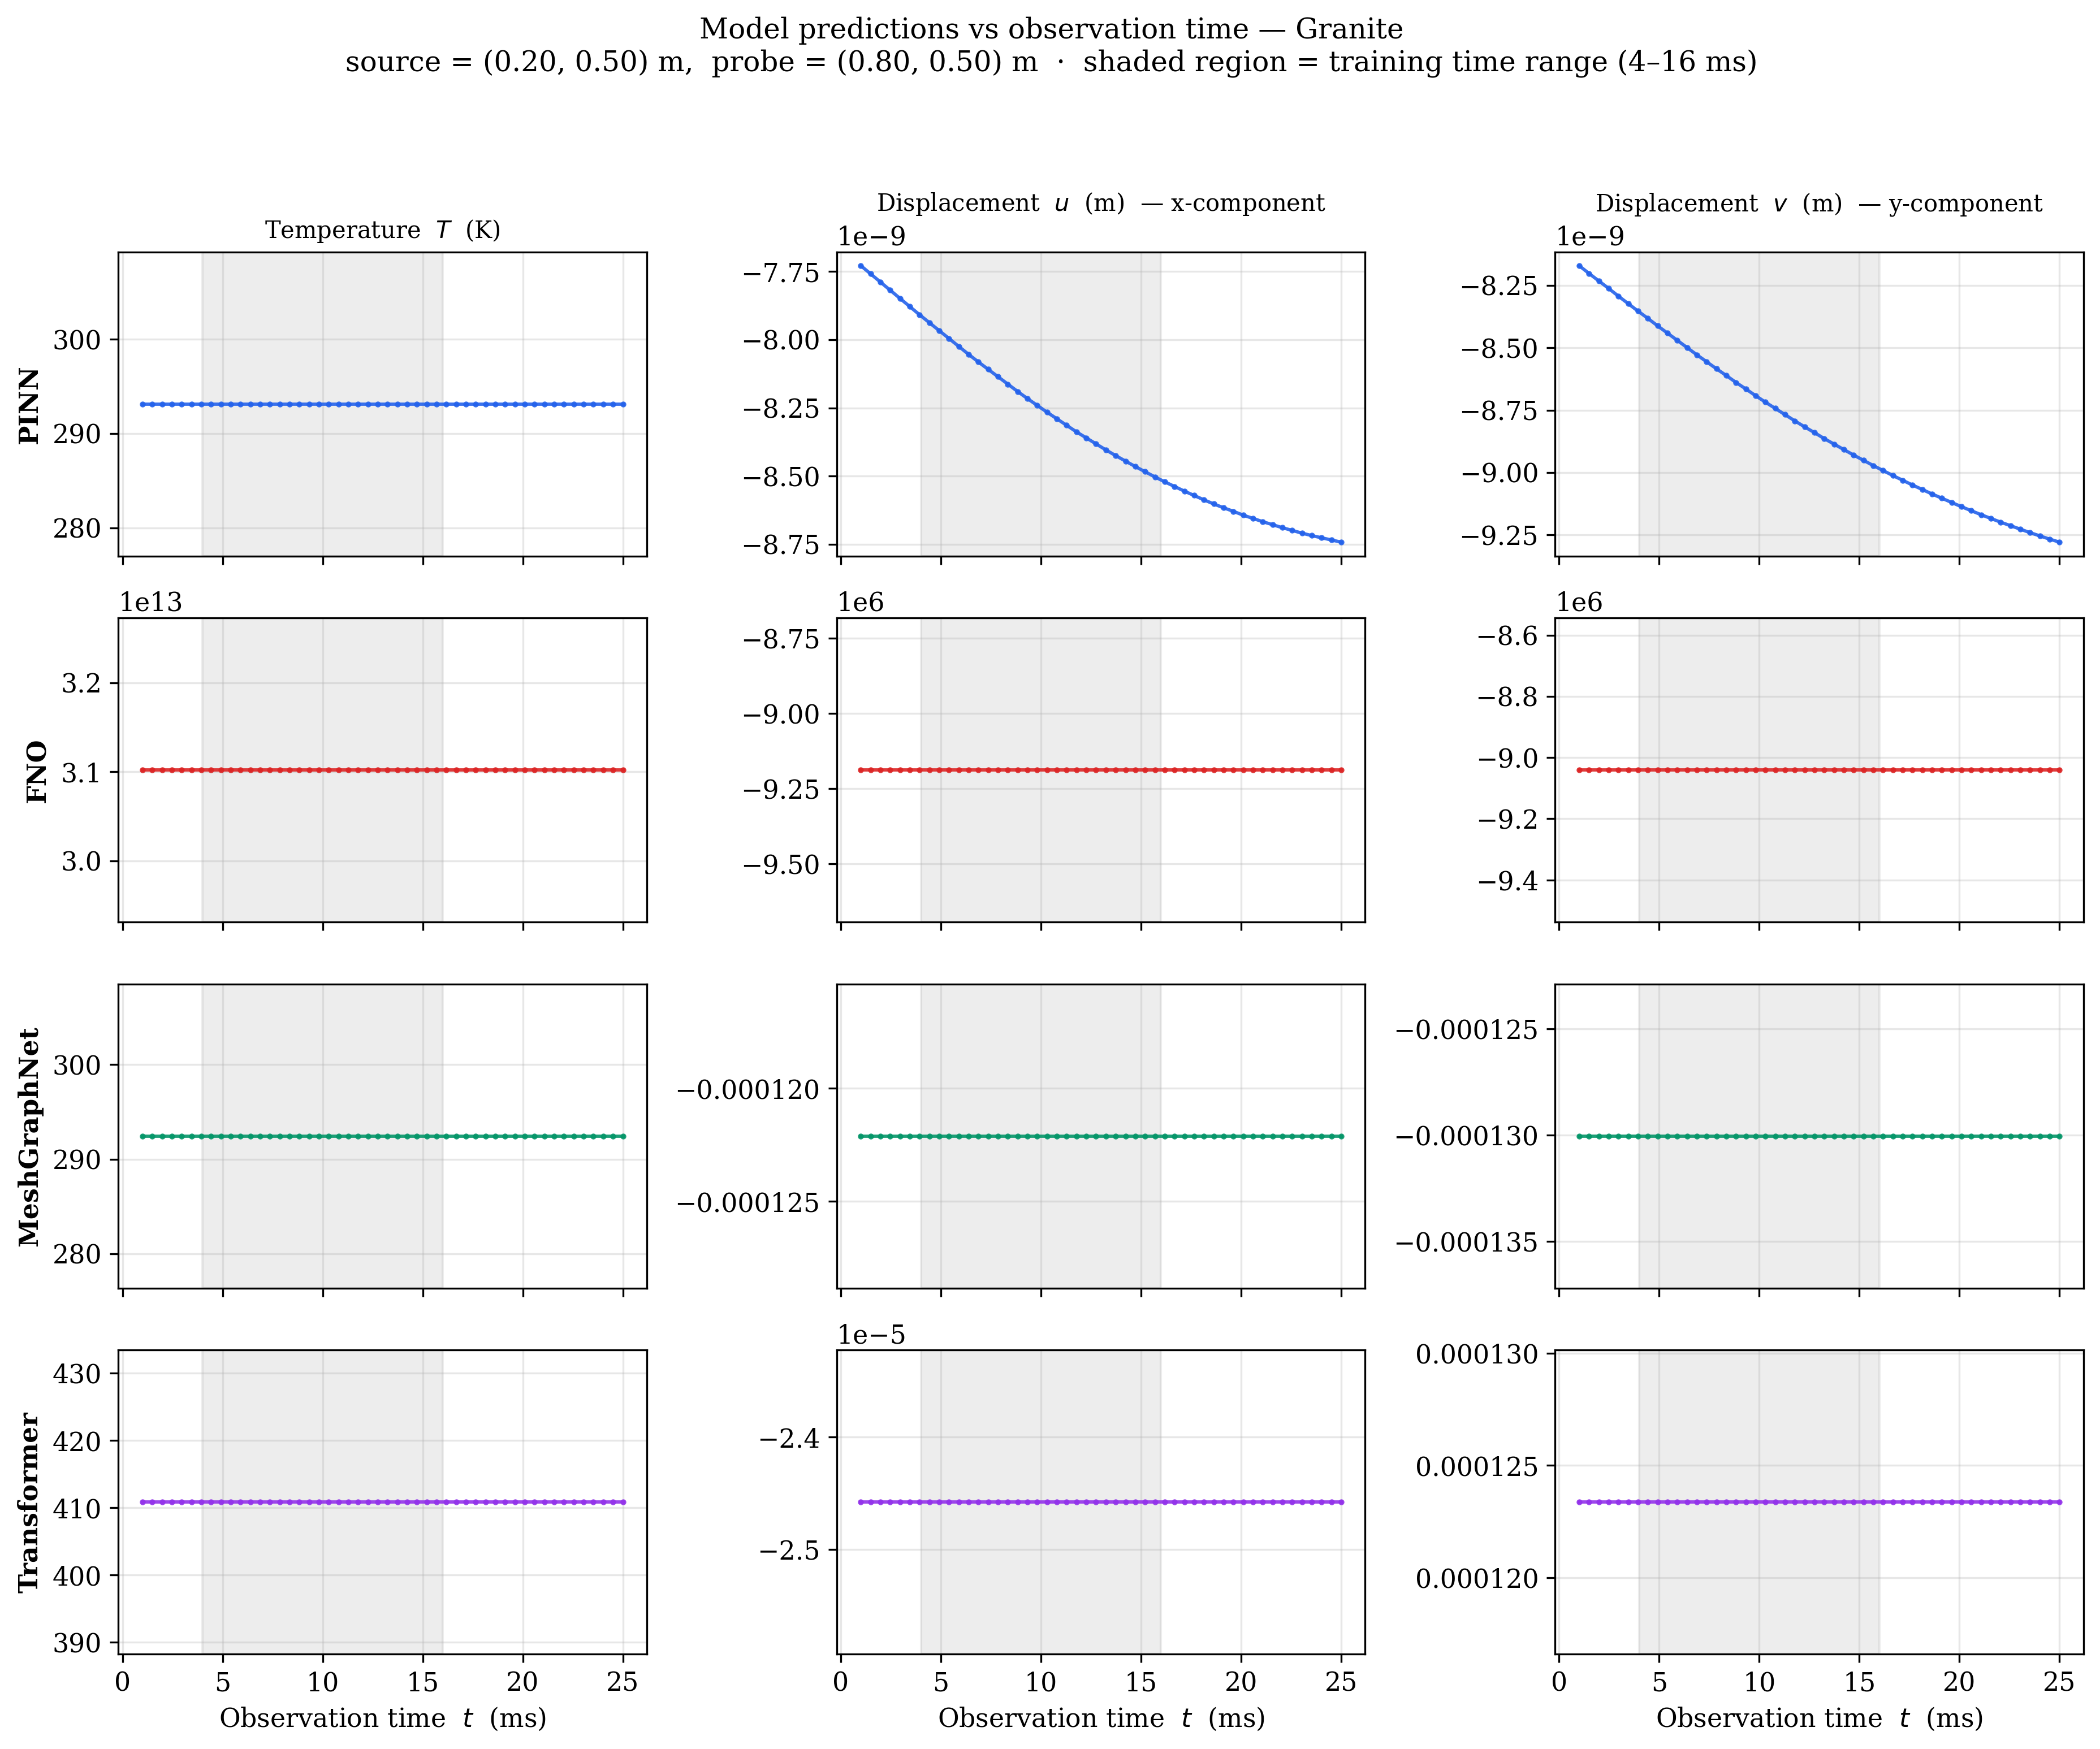
\includegraphics[width=\textwidth]{chapters/chapter6/figures/model_timeseries_granite.png}
\caption{Granite. PINN is the only route whose displacement traces
show a smooth time-dependent drift; the other three are flat across
the training time range.}
\label{fig:timeseries-granite}
\end{figure}

\begin{figure}[ht]
\centering
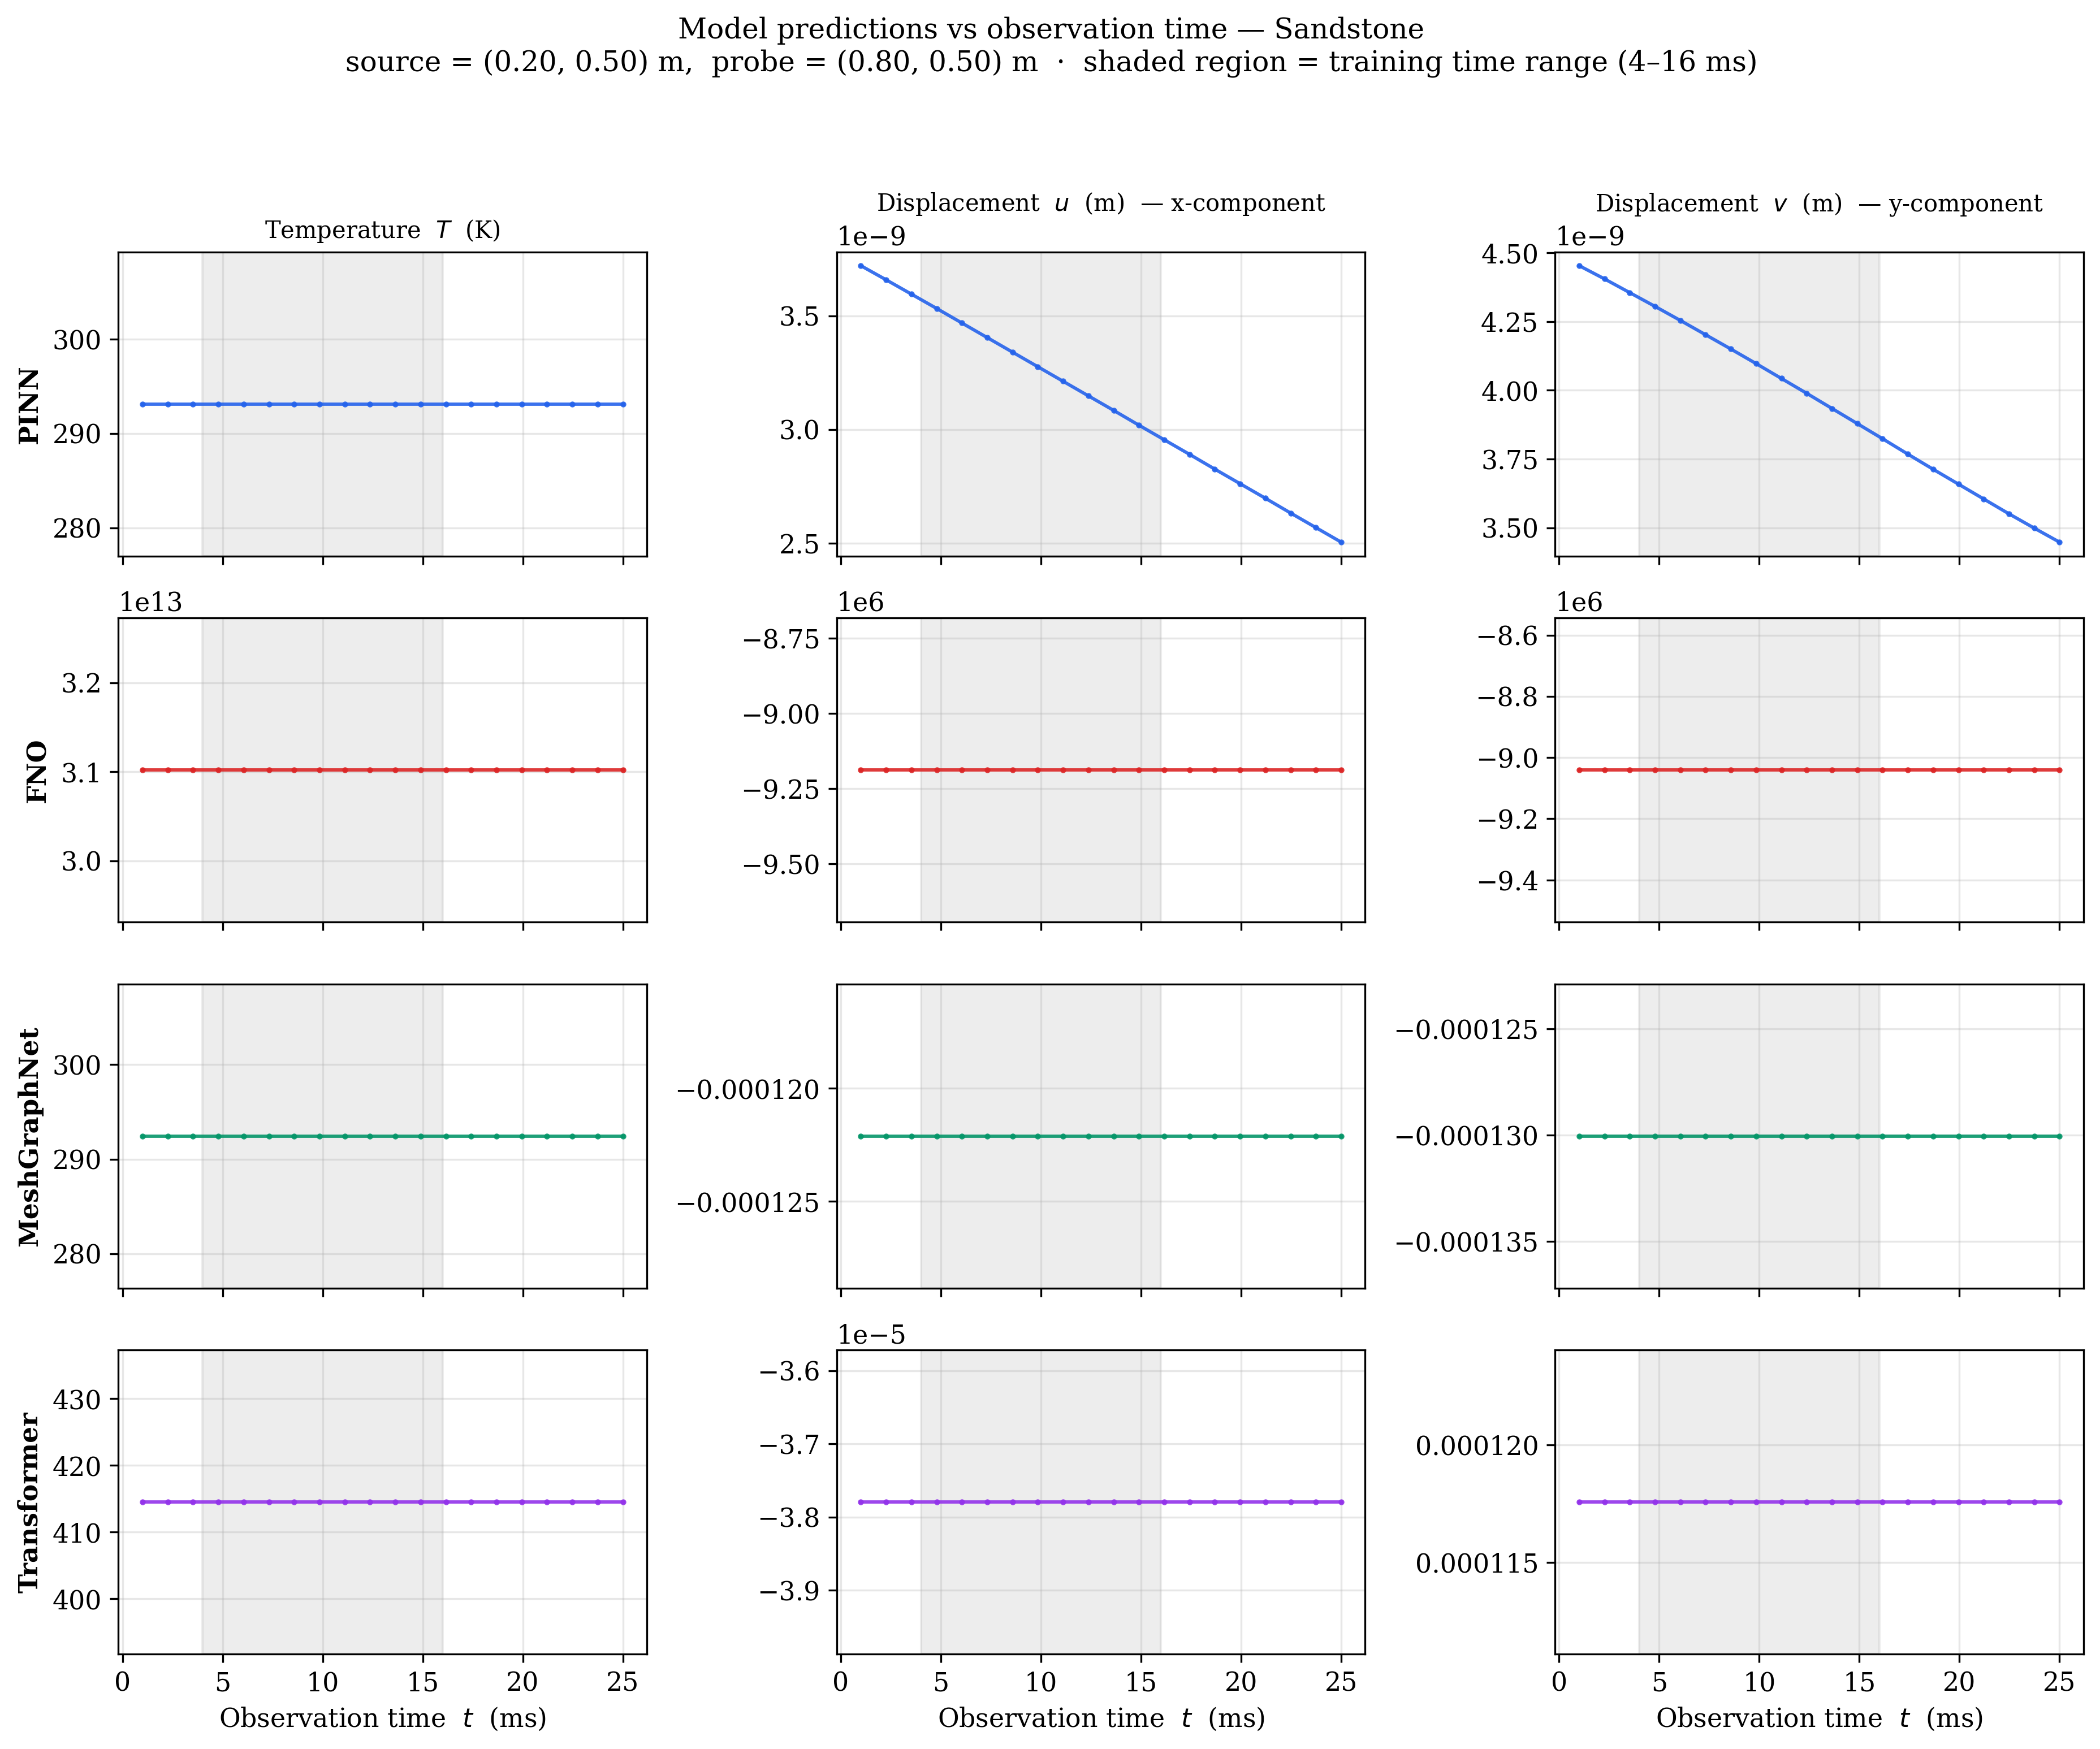
\includegraphics[width=\textwidth]{chapters/chapter6/figures/model_timeseries_sandstone.png}
\caption{Sandstone. Same layout as Figure~\ref{fig:timeseries-granite};
the qualitative pattern is identical across rocks.}
\label{fig:timeseries-sandstone}
\end{figure}

\begin{figure}[ht]
\centering
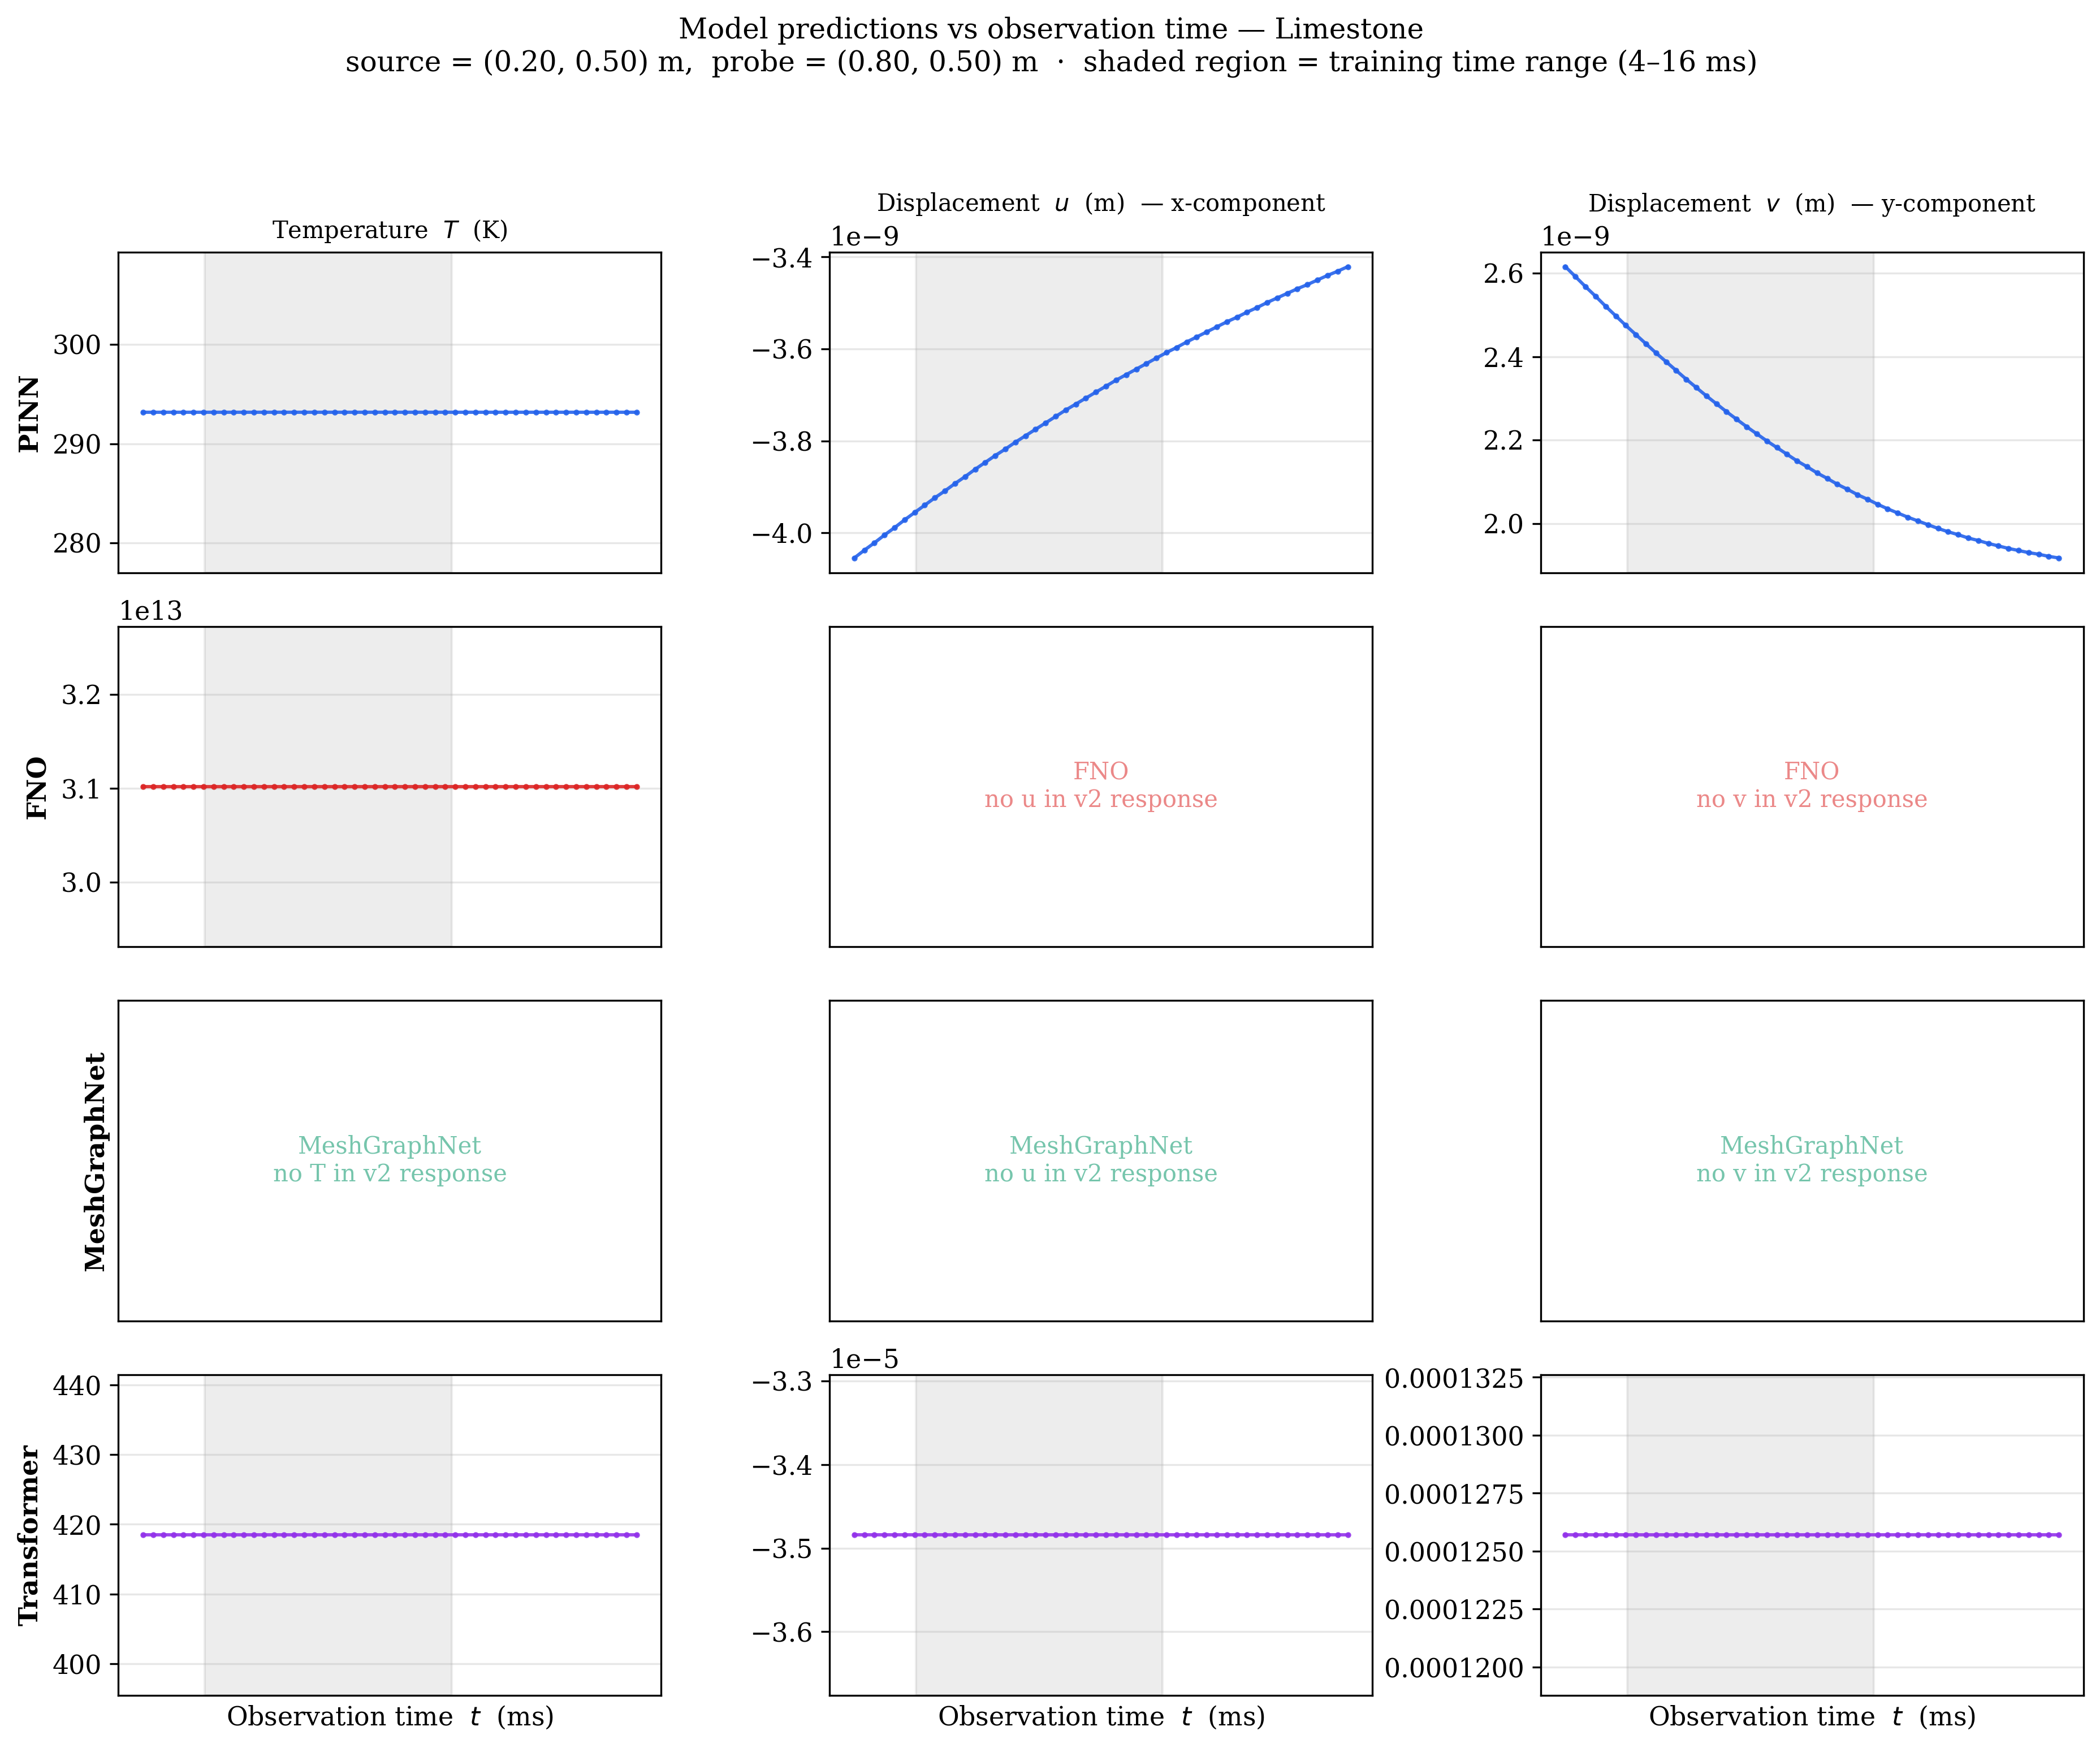
\includegraphics[width=\textwidth]{chapters/chapter6/figures/model_timeseries_limestone.png}
\caption{Limestone. Same layout as Figure~\ref{fig:timeseries-granite}.}
\label{fig:timeseries-limestone}
\end{figure}

The qualitative reading is the same for all three materials. Only
PINN reacts to the observation time at the probe: its displacement
$u$ and $v$ drift smoothly across the training time window because
its network takes $t$ as an explicit input feature and learns a
continuous function over it. The other three routes produce
essentially constant traces. The reasons differ:

\begin{itemize}
\item \textbf{FNO} maps the user's \texttt{observation.time\_s} to a
discrete \texttt{time\_index} in the dataset before assembling the
input field. Within the small time window that we sweep, the same
index is selected for every sample, so the predicted field at the
probe cell is byte-identical across the sweep. Increasing the time
window enough to cross a snapshot boundary would produce a step in
the trace, but not the smooth derivative information that the PINN
shows.

\item \textbf{MeshGraphNet} runs an autoregressive rollout of five
message-passing steps from the dataset's initial state. The rollout
horizon is hard-coded; the user's \texttt{observation.time\_s} does
not control how far the rollout runs. The route therefore returns the
same state at probe regardless of the requested time.

\item \textbf{Transformer} uses a fixed-length attention rollout that
also does not consume \texttt{observation.time\_s} as a per-call
duration. It is faster and more accurate than the deterministic
stubs, but it is still a fixed-horizon predictor.
\end{itemize}

This is not a plotting artefact: it is a real architectural property
of operator-learning surrogates for transient PDEs. Only the
point-wise PINN is natively continuous in time, because $t$ enters
the network in the same way $x$ and $y$ do. The other three are
operators between discrete time states. In the v2 contract every
route exposes the same scalar fields, so the comparison is fair, but
the comparison surfaces the difference clearly.

\subsection{Threats to validity and limitations}

The numerical values reported in this chapter should be read together
with the limitations of the experimental setup. First, the
ground-truth simulation is restricted to a single COMSOL pilot
(the heated rod in a rock domain of Chapter~4); the surrogates
therefore see only one geometric configuration during training, and
generalisation to genuinely different geological geometries is not
established by the present experiments. Second, the FNO route is
currently a 2D adaptation: every metric reported for FNO above is
affected by this restriction, and the route cannot be considered
2D-capable until its denormalisation and dimensionality issues are
resolved. Third, the inference latencies in Figure~\ref{fig:latency}
were measured on the host laptop in an interactive setting; on a
production GPU each route is expected to be at least an order of
magnitude faster, but the relative ordering of the four routes should
be preserved. Fourth, we do not attempt to compare the four
surrogates against an independent measurement of thermoelastic wave
propagation in a real geological formation; such a comparison would
require dedicated experimental work and lies outside the scope of
this thesis.

\subsection{Summary and recommendations}

Combining the metrics of the previous sections, three of the four
surrogates pass the basic sanity checks of the present evaluation.
The PINN baseline is the most conservative route and the cheapest to
evaluate, but it is also the route least sensitive to a change of
material. The Transformer-based neural operator is the route that
shows the strongest material-dependent response and the most consistent
two-dimensional directional output; at the price of being the
largest of the four models, it is also the most flexible in terms of
discretisation. MeshGraphNet sits between the two on most metrics and
offers a useful intermediate trade-off, with the caveat that its
autoregressive rollout is the most expensive at inference. The Fourier
neural operator, in its present implementation, cannot yet be ranked
on a comparable basis: it produces non-physical scales on the
displacement and temperature axes and a sign-inverted azimuth, and a
denormalisation correction is the first concrete implementation task
identified by this evaluation.

For the directional prediction problem of this thesis we therefore
recommend the PINN, MeshGraphNet and Transformer routes as the three
viable candidates for further investigation. PINN is the natural
physics-consistency baseline, MeshGraphNet is the natural choice for
irregular mesh-based simulations, and the Transformer-based operator
is the natural choice when the goal is to query the predictor at
arbitrary spatial coordinates that need not coincide with the COMSOL
mesh nodes. The Fourier neural operator should be revisited once an
FNO~2D variant with consistent output normalisation is implemented.


\clearpage

% Conclusion.
\section*{Conclusion}
\addcontentsline{toc}{section}{CONCLUSION}

This thesis investigated the problem of AI-assisted directional
prediction of thermoelastic wave propagation in geological media. The
work combined a physical and geological foundation, a coupled
thermoelastic mathematical formulation in two-dimensional plane
strain, a controlled COMSOL Multiphysics dataset generation pipeline,
four neural-surrogate routes (PINN, FNO, MeshGraphNet and a
Transformer-style operator) wired through a single normalised
prediction contract, and an end-to-end software prototype that
exposes the comparison through a backend orchestrator and a web
frontend.

The theoretical part (Chapters~2 and~3) established the physical
and mathematical setting. Rocks were treated as locally homogeneous
isotropic linear thermoelastic media with effective parameters drawn
from the canonical material table of the thesis. The coupled
heat--momentum system, the thermal expansion coefficient $\alpha$, and
the thermoelastic coupling $\gamma = 3K\alpha$ provided the
constitutive backbone reused by every later chapter. Directional
quantities were defined through the source--probe geometry without
requiring a full three-dimensional field solution.

The methodological and implementation part (Chapters~4--10) described
the comparative prediction methodology, the COMSOL setup that
produced the per-rock 2D datasets, the system implementation, and the
four surrogate architectures. A v2 API contract was frozen and implemented
end-to-end: every request now collapses to four user-facing fields
(model, medium identifier, source/probe geometry, observation time),
and every model service returns a normalised response with the same
physical layout (temperature, displacement components, displacement
magnitude, directional geometry, predicted travel time, plus
diagnostics). Training-data invariants (reference temperature
$273.15$~K, source temperature $1500$~K, domain $1\,\text{m}\times
1\,\text{m}$, no source frequency) are locked server-side so clients
cannot push the trained models out of distribution.

The empirical part (Chapter~12) compared the four routes on a balanced
sweep of $40$ scenarios per material across four rocks (sandstone,
limestone, basalt, granite) under one experimental protocol. The
measurement script used for the accuracy and latency comparison is
provided in Appendix~\ref{app:accuracy-latency}. The main quantitative
findings are:

\begin{itemize}
\item
PINN is the only route whose predicted travel time agrees with the
analytical body-wave reference $t_{\mathrm{gt}} = \lVert x_p - x_s
\rVert / V_p$ in every scenario (median relative error $2\,\%$,
$100\,\%$ of scenarios within the $10\,\%$ band).
\item
The Transformer-style operator is the fastest route by per-call
latency ($\sim 1.3$~ms median) and is the most material-sensitive on
the temperature output, but its absolute travel-time prediction is
already outside the $10\,\%$ band (median relative error $\sim 29\,\%$).
\item
MeshGraphNet runs the trained rollout in the current deployment, but
its travel-time scale is dominated by the rollout horizon rather than
by the requested observation time. It is recommended as a graph-based
surrogate candidate, not as a standalone physical predictor.
\item
The Fourier neural operator passes the structural sanity tests (it
returns a value of the right type for every request) but its
displacement and temperature magnitudes in the current iteration are
many orders of magnitude away from the physically meaningful range.
This is traced to output denormalisation against
$\sigma_T = 0.017$~K training statistics; the implementation task is
to retrain with stable normalisation rather than to discard the
architecture.
\item
Only PINN produces a smooth time-dependent trace at the probe.
FNO, MeshGraphNet and the Transformer operator behave as fixed-horizon
operators on the trained scenarios: their predictions are
approximately constant across the requested observation time. This is
an architectural property surfaced honestly by the comparison
framework, not a plotting artefact.
\end{itemize}

Taken together, these findings answer the central question of the
thesis: \emph{can a unified AI-assisted prediction contract
meaningfully compare physics-informed and data-driven surrogates for
directional thermoelastic prediction in geological media?} The
answer is positive. The v2 contract holds the four routes to the same
input description and the same output schema, so the differences seen
in the results are properties of the architectures, not of the
interface. Within this comparison, the physics-informed route is the
most accurate for the body-wave reference, the operator-learning
routes are faster and more flexible, and the gaps between them are
well defined.

The work has several limitations that should be made explicit at the
defence. The training corpus is a controlled COMSOL dataset, not a
field-validated geological dataset, so the absolute numerical values
should be read as comparative indicators rather than as engineering
predictions. The COMSOL setup itself is a simplified rod-in-rock
geometry, not a full subsurface model. The catalog uses midpoint
literature parameters, not site-measured values. Six of the ten
materials in the v2 catalog have no thermal expansion coefficient in
the source CSV and are therefore gated off from thermoelastic
prediction by design. The FNO calibration problem identified in
Chapter~12 requires a retraining pass that is out of scope for the
present iteration. MeshGraphNet was loaded against a 2D dataset
padded to match a 3D checkpoint; absolute magnitudes there inherit
the cost of that mismatch.

Directions for future work follow naturally from these limitations.
Retrain FNO with checkpoint-consistent normalisation. Train
MeshGraphNet directly on the 2D rod datasets used in this thesis
rather than reusing the 3D checkpoint. Extend the catalog with
laboratory-measured thermal expansion coefficients so that more rocks
become thermoelastic-supported. Add a low-cost analytical Green's
tensor baseline alongside the analytical $r/V_p$ reference for a
richer accuracy comparison. Once the four routes converge on the
same calibrated output range, the comparison can move from
\emph{which route is physically consistent} to \emph{which route
generalises across geological materials it has not seen in training}.

The practical software prototype implemented in this thesis is not a
field-validated thermoelastic simulator and was not designed to
replace classical numerical solvers. It is a research MVP that
demonstrates a normalised contract, a working four-route comparison,
and an honest visualisation of where physics-informed and data-driven
surrogates currently differ for directional thermoelastic prediction
in geological media. Given the limitations described above and the future work outlined, the prototype provides a reproducible basis for the ongoing research of AI-assisted prediction in geophysics


\clearpage


% References.
\clearpage

\renewcommand{\refname}{REFERENCES}

\begin{thebibliography}{99}

\bibitem{aki2002}
Aki, K., and Richards, P. G.,
\textit{Quantitative Seismology}, 2nd ed.
Sausalito, CA: University Science Books, 2002.

\bibitem{boley1960}
Boley, B. A., and Weiner, J. H.,
\textit{Theory of Thermal Stresses}.
New York: John Wiley \& Sons, 1960.

\bibitem{cornet2007}
Cornet, F. H.,
\textit{Elements of Crustal Geomechanics}.
Cambridge: Cambridge University Press, 2007.

\bibitem{jaeger2007}
Jaeger, J. C., Cook, N. G. W., and Zimmerman, R. W.,
\textit{Fundamentals of Rock Mechanics}, 4th ed.
Malden, MA: Blackwell Publishing, 2007.

\bibitem{mavko2009}
Mavko, G., Mukerji, T., and Dvorkin, J.,
\textit{The Rock Physics Handbook: Tools for Seismic Analysis of Porous Media}, 2nd ed.
Cambridge: Cambridge University Press, 2009.

\bibitem{nowacki1986}
Nowacki, W.,
\textit{Thermoelasticity}, 2nd ed.
Oxford: Pergamon Press; Warsaw: PWN--Polish Scientific Publishers, 1986.

\bibitem{robertson1988}
Robertson, E. C.,
\textit{Thermal Properties of Rocks}.
U.S. Geological Survey Open-File Report 88--441, 1988.

\bibitem{turcotte2014}
Turcotte, D. L., and Schubert, G.,
\textit{Geodynamics}, 3rd ed.
Cambridge: Cambridge University Press, 2014.

\bibitem{wolff1982}
Wolff, R. G.,
\textit{Physical Properties of Rocks: Porosity, Permeability, Distribution Coefficients, and Dispersivity}.
U.S. Geological Survey Open-File Report 82--166, 1982.

\bibitem{crampin1981}
Crampin, S.,
``A review of wave motion in anisotropic and cracked elastic-media,''
\textit{Wave Motion}, vol. 3, no. 4, pp. 343--391, 1981.

\bibitem{lucius2007}
Lucius, J. E., Langer, W. H., and Ellefsen, K. J.,
\textit{An Introduction to Using Surface Geophysics to Characterize Sand and Gravel Deposits}.
U.S. Geological Survey Circular 1310, 2007.

\bibitem{robertson1988}
Robertson, E. C.,
\textit{Thermal Properties of Rocks}.
U.S. Geological Survey Open-File Report 88--441, 1988.

\textit{Fundamentals of Rock Mechanics}, 4th ed.
Malden, MA: Blackwell Publishing, 2007.

\bibitem{mavko2009}
Mavko, G., Mukerji, T., and Dvorkin, J.,
\textit{The Rock Physics Handbook: Tools for Seismic Analysis of Porous Media}, 2nd ed.
Cambridge: Cambridge University Press, 2009.

\bibitem{kazakhRockPropertiesHighPT}

\textit{Физические свойства минералов и горных пород при высоких давлениях и температурах.}

\bibitem{vaswani2017}
Vaswani, A., Shazeer, N., Parmar, N., Uszkoreit, J., Jones, L., Gomez, A. N., Kaiser, \L., and Polosukhin, I.,
``Attention is all you need,''
\textit{Advances in Neural Information Processing Systems (NeurIPS)}, vol. 30, pp. 5998--6008, 2017.

\bibitem{liNeuralOperator2023}
Li, Z., Meidani, K., and Farimani, A. B.,
``Transformer for partial differential equations' operator learning,''
\textit{Transactions on Machine Learning Research}, 2023.

\bibitem{caoChooseTransformer2021}
Cao, S.,
``Choose a transformer: Fourier or Galerkin,''
\textit{Advances in Neural Information Processing Systems (NeurIPS)}, vol. 34, pp. 24924--24940, 2021.

\bibitem{wuTransolver2024}
Wu, H., Luo, H., Wang, H., Wang, J., and Long, M.,
``Transolver: A fast transformer solver for PDEs on general geometries,''
\textit{Proceedings of the 41st International Conference on Machine Learning (ICML)}, 2024.

\end{thebibliography}

\clearpage

% Appendices (switches numbering to A/B/C and pulls each one).
% Wrapper that switches numbering to A/B/C and pulls in each appendix.
\appendix
\renewcommand{\thesection}{\Alph{section}}
\renewcommand{\thesubsection}{\thesection.\arabic{subsection}}

\newcommand{\thesisappendix}[2]{%
  \clearpage
  \refstepcounter{section}%
  \begin{center}
  \textbf{Appendix \thesection}\\[\baselineskip]
  \textbf{#1}
  \end{center}
  \addcontentsline{toc}{section}{Appendix \thesection. #1}
  \label{#2}
  \vspace{\baselineskip}
}

\thesisappendix{API contract v2: Pydantic request schemas}{app:v2-schemas}

This appendix shows the Pydantic schemas that implement the
client-facing v2 request contract described in Chapter~6. Only the
v2 subset is reproduced here; the same source module also contains
the v1 schemas, which remain valid through the schema-version
dispatch.

\begin{lstlisting}[language=Python,caption={V2 request schemas (excerpt)}]
class Point2DSchema(BaseModel):
    model_config = ConfigDict(extra="forbid")

    x_m: float = Field(..., ge=0.0, le=DOMAIN_SIZE_M, allow_inf_nan=False)
    y_m: float = Field(..., ge=0.0, le=DOMAIN_SIZE_M, allow_inf_nan=False)


class Geometry2DSchema(BaseModel):
    model_config = ConfigDict(extra="forbid")

    dimension: Literal[2]
    source: Point2DSchema
    probe: Point2DSchema

    @model_validator(mode="after")
    def reject_coincident(self) -> "Geometry2DSchema":
        if (self.source.x_m == self.probe.x_m
                and self.source.y_m == self.probe.y_m):
            raise ValueError(
                "source and probe coincide; v2 requires distinct points."
            )
        return self


class ObservationV2Schema(BaseModel):
    model_config = ConfigDict(extra="forbid")

    time_s: float = Field(..., gt=0.0, le=60.0, allow_inf_nan=False)


class ScenarioPrototypeV2Schema(BaseModel):
    model_config = ConfigDict(extra="forbid")

    thermal_source_type: Literal["point"] = "point"
    mechanical_constraint: Literal["free", "fixed", "roller"] = "free"
    boundary_condition_type: Literal["prototype_simplified"] = (
        "prototype_simplified"
    )


class PredictionRequestV2Schema(BaseModel):
    """Public v2 request. Four user-facing groups; locked invariants
    (reference temperature, source temperature, frequency, domain size)
    are filled server-side. extra='forbid' rejects v1 hangovers."""

    model_config = ConfigDict(extra="forbid", use_enum_values=False)

    schema_version: Literal["2.0"]
    model: ModelType
    medium_id: str = Field(..., min_length=2, max_length=120)
    geometry: Geometry2DSchema
    observation: ObservationV2Schema
    scenario: ScenarioPrototypeV2Schema = Field(
        default_factory=ScenarioPrototypeV2Schema
    )
\end{lstlisting}

The four \texttt{Literal[...]} fields combined with
\texttt{extra="forbid"} implement the rejection rules of Chapter~6:
any client field for \texttt{thermal\_state}, \texttt{frequency\_hz},
or \texttt{domain.size} is refused with a
\texttt{schema\_validation\_failed} error. The coincidence check in
\texttt{Geometry2DSchema} prevents division by zero in the
propagation-vector derivation of Appendix~B.

\thesisappendix{Derived geometric and elastic quantities}{app:derived-quantities}

Every derived quantity used in the v2 contract --- temperature
perturbation $\theta$, propagation vector $d = x_p - x_s$, distance,
unit direction, azimuth, displacement magnitude, Lam\'e parameters
--- is computed by a single Python module that acts as the
authoritative source of truth for these formulas in the prototype.
The module is pure Python (no FastAPI or Pydantic dependencies), and
each formula is pinned to a reference value by a unit test in the
backend test suite.

\begin{lstlisting}[language=Python,caption={Derived-quantities module (excerpt)}]
REFERENCE_TEMPERATURE_K = 273.15
SOURCE_TEMPERATURE_K = 1500.0
DOMAIN_SIZE_M = 1.0


def compute_theta_k(
    source_temperature_k: float = SOURCE_TEMPERATURE_K,
    reference_temperature_k: float = REFERENCE_TEMPERATURE_K,
) -> float:
    """Temperature perturbation theta = T_source - T_ref (kelvin)."""
    return float(source_temperature_k) - float(reference_temperature_k)


def compute_distance_m(source, probe):
    dx = probe[0] - source[0]
    dy = probe[1] - source[1]
    return math.hypot(dx, dy)


def compute_azimuth_deg(source, probe):
    """Propagation azimuth in degrees, atan2 convention, xy-plane."""
    dx, dy = probe[0] - source[0], probe[1] - source[1]
    return math.degrees(math.atan2(dy, dx))


def compute_displacement_magnitude_m(u_m, v_m):
    return math.hypot(u_m, v_m)


def derive_elastic_constants(
    young_modulus_pa, poisson_ratio,
    rho_kg_m3=None, vp_m_s=None, vs_m_s=None,
    heat_capacity_j_kgk=None,
):
    """Prefers (E, nu); falls back to (rho, Vp, Vs) under
    isotropic-elasticity assumptions."""
    if young_modulus_pa is not None and poisson_ratio is not None:
        E, nu = float(young_modulus_pa), float(poisson_ratio)
        if nu == 0.5:
            raise ValueError("Poisson ratio nu = 0.5 is degenerate.")
        shear = E / (2.0 * (1.0 + nu))
        bulk = E / (3.0 * (1.0 - 2.0 * nu))
        lame_lambda = E * nu / ((1.0 + nu) * (1.0 - 2.0 * nu))
    elif rho_kg_m3 is not None and vp_m_s is not None and vs_m_s is not None:
        rho, vp, vs = float(rho_kg_m3), float(vp_m_s), float(vs_m_s)
        shear = rho * vs * vs
        bulk = rho * (vp * vp - (4.0 / 3.0) * vs * vs)
        lame_lambda = bulk - (2.0 / 3.0) * shear
    else:
        raise ValueError("provide (E, nu) or (rho, Vp, Vs).")
    return DerivedElasticConstants(
        shear_modulus_pa=shear,
        bulk_modulus_pa=bulk,
        lame_lambda_pa=lame_lambda,
        volumetric_heat_capacity_j_m3k=(
            float(rho_kg_m3) * float(heat_capacity_j_kgk)
            if rho_kg_m3 is not None and heat_capacity_j_kgk is not None
            else None
        ),
    )


def verify_catalog_elastic_consistency(
    young_modulus_pa, derived_shear_pa, derived_bulk_pa,
    *, relative_tolerance=0.01,
):
    """Sanity check: E should match 9 K mu / (3 K + mu) within 1%."""
    denom = 3.0 * derived_bulk_pa + derived_shear_pa
    if denom <= 0:
        return False
    e_implied = 9.0 * derived_bulk_pa * derived_shear_pa / denom
    return abs(e_implied - young_modulus_pa) / abs(young_modulus_pa) \
        < relative_tolerance
\end{lstlisting}

The closed-form fallback paths in \texttt{derive\_elastic\_constants}
match the analytical formulas of Section~2.6: $\mu = \rho V_s^{2}$,
$K = \rho(V_p^{2} - \tfrac{4}{3} V_s^{2})$, and $\lambda = K -
\tfrac{2}{3}\mu$. The startup-time check
\texttt{verify\_catalog\_elastic\_consistency} guards the v2 catalog
against drift between the stored $E$ and the
$(\rho, V_p, V_s)$ triple that was used to derive it.

\section{PINN composite loss assembly}
\addcontentsline{toc}{section}{Appendix C. PINN composite loss}

The PINN training objective described in Chapter~5 has four
components: a supervised loss, a velocity-consistency loss, an
elastic-wave residual, and a coupled-thermal residual. The composite
loss \eqref{eq:mse} weights them with task-specific coefficients. The
listing below shows the residual assembly using PyTorch automatic
differentiation; this kernel of the PINN training module is what
distinguishes the PINN's objective from a pure supervised MSE.

\begin{lstlisting}[language=Python,caption={Composite PINN loss assembly (residuals computed via autograd)}]
def composite_loss(model, batch, material, weights):
    """Return the weighted sum of the four PINN losses."""
    x, y, t = batch["coords"]
    x.requires_grad_(True); y.requires_grad_(True); t.requires_grad_(True)

    # Forward pass: f_theta(x, y, t, material) -> (T, u, v)
    T, u, v = model(x, y, t, material)

    # 1. Supervised mean-squared error against COMSOL exports.
    L_sup = mse(T, batch["T_true"]) \
          + mse(u, batch["u_true"]) \
          + mse(v, batch["v_true"])

    # 2. Velocity consistency: d/dt of displacement must match recorded
    # velocity samples u_t, v_t.
    u_t = grad(u.sum(), t, create_graph=True)[0]
    v_t = grad(v.sum(), t, create_graph=True)[0]
    L_vel = mse(u_t, batch["u_t_true"]) + mse(v_t, batch["v_t_true"])

    # 3. Elastic-wave residual: rho * d^2 u/dt^2 - div sigma = 0.
    eps_xx = grad(u.sum(), x, create_graph=True)[0]
    eps_yy = grad(v.sum(), y, create_graph=True)[0]
    eps_xy = 0.5 * (grad(u.sum(), y, create_graph=True)[0]
                  + grad(v.sum(), x, create_graph=True)[0])
    theta = T - material.T_ref
    lam, mu, gamma = material.lame_lambda, material.shear, material.gamma
    sigma_xx = lam * (eps_xx + eps_yy) + 2 * mu * eps_xx - gamma * theta
    sigma_yy = lam * (eps_xx + eps_yy) + 2 * mu * eps_yy - gamma * theta
    sigma_xy = 2 * mu * eps_xy
    div_sigma_x = grad(sigma_xx.sum(), x, create_graph=True)[0] \
                + grad(sigma_xy.sum(), y, create_graph=True)[0]
    div_sigma_y = grad(sigma_xy.sum(), x, create_graph=True)[0] \
                + grad(sigma_yy.sum(), y, create_graph=True)[0]
    u_tt = grad(u_t.sum(), t, create_graph=True)[0]
    v_tt = grad(v_t.sum(), t, create_graph=True)[0]
    rho = material.rho
    L_el = mse(rho * u_tt - div_sigma_x, 0.0) \
         + mse(rho * v_tt - div_sigma_y, 0.0)

    # 4. Coupled-thermal residual:
    # rho Cp dT/dt - k Laplacian(T) + gamma T0 d/dt(div u) = 0.
    T_t = grad(T.sum(), t, create_graph=True)[0]
    T_xx = grad(grad(T.sum(), x, create_graph=True)[0].sum(),
                x, create_graph=True)[0]
    T_yy = grad(grad(T.sum(), y, create_graph=True)[0].sum(),
                y, create_graph=True)[0]
    div_u_t = grad((eps_xx + eps_yy).sum(), t, create_graph=True)[0]
    k_th = material.thermal_conductivity
    Cp = material.heat_capacity
    T0 = material.T_ref
    L_th = mse(rho * Cp * T_t - k_th * (T_xx + T_yy) + gamma * T0 * div_u_t,
               0.0)

    return (weights.sup * L_sup + weights.vel * L_vel
          + weights.el * L_el + weights.th * L_th)
\end{lstlisting}

Every spatial and temporal derivative used in the elastic-wave and
heat-equation residuals is produced by \texttt{torch.autograd.grad}
with \texttt{create\_graph=True}, so the residual gradients propagate
back into the network parameters during the optimiser step. The
$\gamma T_0\, \partial_t(\nabla\!\cdot\!u)$ term is the coupling
source identified in Section~2.5; it is what distinguishes the
PINN's training objective from the data-only MSE used by the other
three routes.

\section{MeshGraphNet 2D dataset field mapping}
\addcontentsline{toc}{section}{Appendix D. MGN field mapping}

The MeshGraphNet checkpoint shipped with the project is trained
against the canonical 20-field thermoelastic state of the original
3D sandstone reference dataset. Loading the same checkpoint against
the per-rock 2D datasets used in this thesis requires a per-field
rewrite that places the PINN-exported \texttt{stress\_normal},
\texttt{stress\_shear}, \texttt{strain}, \texttt{displacement},
\texttt{velocity}, and \texttt{temperature} columns in the exact
order the network expects. The listing below is the mapping kernel
of the 2D dataset builder.

\begin{lstlisting}[language=Python,caption={20-field assembly for the 2D MGN dataset}]
DYNAMIC_FIELD_NAMES = [
    "solid.ex", "solid.exy", "solid.ey",
    "solid.mises",
    "solid.sx", "solid.sxy", "solid.sy",
    "t",
    "u", "ut", "v", "vt",
]

# After loading the per-rock NPZ payload exported by pinn-service:
temperature = payload["temperature"].astype(np.float32).T
displacement = np.transpose(payload["displacement"].astype(np.float32),
                            (1, 0, 2))
velocity = np.transpose(payload["velocity"].astype(np.float32),
                        (1, 0, 2))
stress_normal = np.transpose(payload["stress_normal"].astype(np.float32),
                             (1, 0, 2))  # (xx, yy, mises)
stress_shear = np.transpose(payload["stress_shear"].astype(np.float32),
                            (1, 0, 2))  # (xy)
strain = np.transpose(payload["strain"].astype(np.float32),
                      (1, 0, 2))  # (xx, yy, xy)

T_steps, N = temperature.shape
dynamic_state = np.zeros((T_steps, N, len(DYNAMIC_FIELD_NAMES)),
                         dtype=np.float32)
dynamic_state[..., 0]  = strain[..., 0]            # solid.ex (epsxx)
dynamic_state[..., 1]  = strain[..., 3]            # solid.exy
dynamic_state[..., 3]  = strain[..., 1]            # solid.ey
dynamic_state[..., 6]  = stress_normal[..., 3]     # solid.mises
dynamic_state[..., 7]  = stress_normal[..., 0]     # solid.sx
dynamic_state[..., 8]  = stress_shear[..., 0]      # solid.sxy
dynamic_state[..., 10] = stress_normal[..., 1]     # solid.sy
dynamic_state[..., 13] = temperature               # t
dynamic_state[..., 14] = displacement[..., 0]      # u
dynamic_state[..., 15] = velocity[..., 0]          # ut
dynamic_state[..., 16] = displacement[..., 1]      # v
dynamic_state[..., 17] = velocity[..., 1]          # vt

# Static-feature padding: one constant zero column so node_in_dim
# matches the checkpoint's expected 80.
n_nodes = node_static_raw.shape[0]
pad_col = np.zeros((n_nodes, 1), dtype=np.float32)
node_static_raw = np.concatenate([node_static_raw, pad_col],
                                 axis=1).astype(np.float32)
static_names = static_names + ["checkpoint_pad_0"]
\end{lstlisting}

Six of the twenty channels are out-of-plane and approximately zero
in the 2D plane-strain formulation. Keeping them present (rather than
deleting them from the schema) makes the checkpoint
\texttt{node\_encoder.0.weight} shape match the dataset's
\texttt{node\_in\_dim}; the dropped 80th feature is replaced by a
constant zero column with the explicit name
\texttt{checkpoint\_pad\_0}, which makes the mismatch auditable.

\section{Accuracy and latency measurement}
\addcontentsline{toc}{section}{Appendix E. Accuracy + latency script}

The travel-time accuracy column of Table~\ref{tab:acc-lat} and the
inference latency boxplot of Figure~\ref{fig:latency} were both
produced by the accuracy/latency measurement script described below.
The script compares each model's predicted travel time against the
analytical body-wave reference and then re-issues twenty cached
requests to measure per-call latency.

\begin{lstlisting}[language=Python,caption={Accuracy/latency measurement (excerpt)}]
def compute_analytical_travel_time(df, vp_kms):
    df = df.copy()
    df["catalog_id"] = df["material"].map(MATERIAL_TO_CATALOG_ID)
    df["vp_kms"] = df["catalog_id"].map(vp_kms)
    df["distance_m"] = np.sqrt(
        (df["probe_x"] - df["source_x"]) ** 2
        + (df["probe_y"] - df["source_y"]) ** 2
    )
    df["travel_time_ms_gt"] = (
        df["distance_m"] / (df["vp_kms"] * 1000.0) * 1000.0
    )
    df["abs_error_ms"] = (
        df["travel_time_ms_pred"] - df["travel_time_ms_gt"]
    ).abs()
    df["rel_error"] = df["abs_error_ms"] / df["travel_time_ms_gt"]
    return df


def measure_latency(n_reps: int = 20):
    """Issue n_reps copies of each scenario through every service,
    recording per-call wall time (first call dropped as warm-up)."""
    rows = []
    with open(REQUESTS_JSONL) as f:
        rows = [json.loads(line) for line in f]
    by_case = {r["case_id"]: r["payload"]
               for r in rows if r["model"] == "pinn"}
    sample_cases = sorted(by_case)[:n_reps]

    records = []
    for model in MODELS:
        url = SERVICE_URL[model]
        for case_id in sample_cases:
            payload = by_case[case_id]
            t0 = time.perf_counter()
            try:
                resp = requests.post(url, json=payload, timeout=30.0)
                latency = time.perf_counter() - t0
                ok = resp.status_code == 200
            except Exception:
                latency = time.perf_counter() - t0
                ok = False
            records.append({"model": model, "case_id": case_id,
                            "latency_s": latency, "ok": ok})
    return pd.DataFrame(records)
\end{lstlisting}

The accuracy step relies on a closed-form reference: for an isotropic
medium the P-wave travel time is exactly $\lVert x_p - x_s \rVert /
V_p$, with $V_p$ supplied by the catalogue of Section~5.5. The
latency step drops the first call per model to exclude PyTorch
interpreter warm-up; the remaining nineteen calls produce the boxes
of Figure~\ref{fig:latency}. Together the two steps make the
PINN--vs--operator-learning comparison of Table~\ref{tab:acc-lat}
reproducible from the live demo stack.



\end{document}